% ******************************* PhD Thesis Template **************************
% Please have a look at the README.md file for info on how to use the template


%\documentclass[a4paper,12pt,times,numbered,print,index]{PhDThesisPSnPDF}
\documentclass[a4paper,12pt,fourier,numbered,print,index]{PhDThesisPSnPDF}
\usepackage{hyperref}
\usepackage{setspace}\onehalfspacing
%\usepackage[superscript,biblabel,nomove]{cite}
% ******************************************************************************
% ******************************* Class Options ********************************
% *********************** See README for more details **************************
% ******************************************************************************

% `a4paper'(The University of Cambridge PhD thesis guidelines recommends a page
% size a4 - default option) or `a5paper': A5 Paper size is also allowed as per
% the Cambridge University Engineering Deparment guidelines for PhD thesis
%
% `11pt' or `12pt'(default): Font Size 10pt is NOT recommended by the University
% guidelines
%
% `oneside' or `twoside'(default): Printing double side (twoside) or single
% side.
%
% `print': Use `print' for print version with appropriate margins and page
% layout. Leaving the options field blank will activate Online version.
%
% `index': For index at the end of the thesis
%
% `draftclassic': For draft mode without loading any images (same as draft in book)
%
% `draft': Special draft mode with line numbers, images, and water mark with
% timestamp and custom text. Position of the text can also be modified.
%
% `abstract': To generate only the title page and abstract page with
% dissertation title and name, to submit to the Student Registry
%
% `chapter`: This option enables only the specified chapter and it's references
%  Useful for review and corrections.
%
% ************************* Custom Page Margins ********************************
%
% `custommargin`: Use `custommargin' in options to activate custom page margins,
% which can be defined in the preamble.tex. Custom margin will override
% print/online margin setup.
%
% *********************** Choosing the Fonts in Class Options ******************
%
% `times' : Times font with math support. (The Cambridge University guidelines
% recommend using times)
%
% `fourier': Utopia Font with Fourier Math font (Font has to be installed)
%            It's a free font.
%
% `customfont': Use `customfont' option in the document class and load the
% package in the preamble.tex
%
% default or leave empty: `Latin Modern' font will be loaded.
%
% ********************** Choosing the Bibliography style ***********************
%
% `authoryear': For author-year citation eg., Krishna (2013)
%
% `numbered': (Default Option) For numbered and sorted citation e.g., [1,5,2]
%
% `custombib': Define your own bibliography style in the `preamble.tex' file.
%              `\RequirePackage[square, sort, numbers, authoryear]{natbib}'.
%              This can be also used to load biblatex instead of natbib
%              (See Preamble)
%
% **************************** Choosing the Page Style *************************
%
% `default (leave empty)': For Page Numbers in Header (Left Even, Right Odd) and
% Chapter Name in Header (Right Even) and Section Name (Left Odd). Blank Footer.
%
% `PageStyleI': Chapter Name next & Page Number on Even Side (Left Even).
% Section Name & Page Number in Header on Odd Side (Right Odd). Footer is empty.
%
% `PageStyleII': Chapter Name on Even Side (Left Even) in Header. Section Number
% and Section Name in Header on Odd Side (Right Odd). Page numbering in footer

% Uncomment to change page style
% pagestyle{PageStyleI}

% ********************************** Preamble **********************************
% Preamble: Contains packages and user-defined commands and settings
% ******************************************************************************
% ****************************** Custom Margin *********************************

% Add `custommargin' in the document class options to use this section
% Set {innerside margin / outerside margin / topmargin / bottom margin}  and
% other page dimensions
\ifsetCustomMargin
  \RequirePackage[left=37mm,right=30mm,top=35mm,bottom=30mm]{geometry}
  \setFancyHdr % To apply fancy header after geometry package is loaded
\fi
\usepackage{adjustbox}
\usepackage{caption}
\usepackage{longtable}
\usepackage{makecell}
\usepackage{floatrow}
% \floatsetup[figure]{capposition=top}
% \usepackage{graphicx,floatrow}
% \captionsetup[table]{position=bottom}

% Add spaces between paragraphs
%\setlength{\parskip}{0.5em}
% Ragged bottom avoids extra whitespaces between paragraphs
\raggedbottom
% To remove the excess top spacing for enumeration, list and description
%\usepackage{enumitem}
%\setlist[enumerate,itemize,description]{topsep=0em}

% *****************************************************************************
% ******************* Fonts (like different typewriter fonts etc.)*************

% Add `customfont' in the document class option to use this section

\ifsetCustomFont
  % Set your custom font here and use `customfont' in options. Leave empty to
  % load computer modern font (default LaTeX font).
  %\RequirePackage{helvet}

  % For use with XeLaTeX
  %  \setmainfont[
  %    Path              = ./libertine/opentype/,
  %    Extension         = .otf,
  %    UprightFont = LinLibertine_R,
  %    BoldFont = LinLibertine_RZ, % Linux Libertine O Regular Semibold
  %    ItalicFont = LinLibertine_RI,
  %    BoldItalicFont = LinLibertine_RZI, % Linux Libertine O Regular Semibold Italic
  %  ]
  %  {libertine}
  %  % load font from system font
  %  \newfontfamily\libertinesystemfont{Linux Libertine O}
\fi

% *****************************************************************************
% **************************** Custom Packages ********************************

% ************************* Algorithms and Pseudocode **************************

%\usepackage{algpseudocode}
\usepackage{amsmath}
\usepackage{mathtools}


% ********************Captions and Hyperreferencing / URL **********************

% Captions: This makes captions of figures use a boldfaced small font.
%\RequirePackage[small,bf]{caption}

\RequirePackage[labelsep=space,tableposition=top]{caption}
\renewcommand{\figurename}{Fig.} %to support older versions of captions.sty


% *************************** Graphics and figures *****************************

%\usepackage{rotating}
%\usepackage{wrapfig}

% Uncomment the following two lines to force Latex to place the figure.
% Use [H] when including graphics. Note 'H' instead of 'h'
%\usepackage{float}
%\restylefloat{figure}

% Subcaption package is also available in the sty folder you can use that by
% uncommenting the following line
% This is for people stuck with older versions of texlive
%\usepackage{sty/caption/subcaption}
\usepackage{subcaption}

% ********************************** Tables ************************************
\usepackage{booktabs} % For professional looking tables
\usepackage{multirow}

%\usepackage{multicol}
%\usepackage{longtable}
%\usepackage{tabularx}


% *********************************** SI Units *********************************
\usepackage{siunitx} % use this package module for SI units



% *********************************** Glossary  *********************************

\usepackage{glossaries}
\PassOptionsToPackage{style=altlong4colheader}{glossaries}

% ******************************* Line Spacing *********************************

% Choose linespacing as appropriate. Default is one-half line spacing as per the
% University guidelines

% \doublespacing
% \onehalfspacing
% \singlespacing


% ************************ Formatting / Footnote *******************************

% Don't break enumeration (etc.) across pages in an ugly manner (default 10000)
%\clubpenalty=500
%\widowpenalty=500

%\usepackage[perpage]{footmisc} %Range of footnote options


% *****************************************************************************
% *************************** Bibliography  and References ********************

%\usepackage{cleveref} %Referencing without need to explicitly state fig /table

% Add `custombib' in the document class option to use this section
\ifuseCustomBib
   \RequirePackage[square, sort, super, numbers, authoryear]{natbib} % CustomBib

% If you would like to use biblatex for your reference management, as opposed to the default `natbibpackage` pass the option `custombib` in the document class. Comment out the previous line to make sure you don't load the natbib package. Uncomment the following lines and specify the location of references.bib file

%\RequirePackage[backend=biber, style=numeric-comp, citestyle=numeric, sorting=nty, natbib=true]{biblatex}
%\addbibresource{References/references} %Location of references.bib only for biblatex, Do not omit the .bib extension from the filename.

\fi

% changes the default name `Bibliography` -> `References'
\renewcommand{\bibname}{References}


% ******************************************************************************
% ************************* User Defined Commands ******************************
% ******************************************************************************

% *********** To change the name of Table of Contents / LOF and LOT ************

%\renewcommand{\contentsname}{My Table of Contents}
%\renewcommand{\listfigurename}{My List of Figures}
%\renewcommand{\listtablename}{My List of Tables}


% ********************** TOC depth and numbering depth *************************

\setcounter{secnumdepth}{3}
\setcounter{tocdepth}{3}


% ******************************* Nomenclature *********************************

% To change the name of the Nomenclature section, uncomment the following line

%\renewcommand{\nomname}{Symbols}


% ********************************* Appendix ***********************************

% The default value of both \appendixtocname and \appendixpagename is `Appendices'. These names can all be changed via:

%\renewcommand{\appendixtocname}{List of appendices}
%\renewcommand{\appendixname}{Appndx}

% *********************** Configure Draft Mode **********************************

% Uncomment to disable figures in `draft'
%\setkeys{Gin}{draft=true}  % set draft to false to enable figures in `draft'

% These options are active only during the draft mode
% Default text is "Draft"
%\SetDraftText{DRAFT}

% Default Watermark location is top. Location (top/bottom)
%\SetDraftWMPosition{bottom}

% Draft Version - default is v1.0
%\SetDraftVersion{v1.1}

% Draft Text grayscale value (should be between 0-black and 1-white)
% Default value is 0.75
%\SetDraftGrayScale{0.8}


% ******************************** Todo Notes **********************************
%% Uncomment the following lines to have todonotes.

%\ifsetDraft
%	\usepackage[colorinlistoftodos]{todonotes}
%	\newcommand{\mynote}[1]{\todo[author=kks32,size=\small,inline,color=green!40]{#1}}
%\else
%	\newcommand{\mynote}[1]{}
%	\newcommand{\listoftodos}{}
%\fi

% Example todo: \mynote{Hey! I have a note}

% ******************************** Highlighting Changes **********************************
%% Uncomment the following lines to be able to highlight text/modifications.
%\ifsetDraft
%  \usepackage{color, soul}
%  \newcommand{\hlc}[2][yellow]{{\sethlcolor{#1} \hl{#2}}}
%  \newcommand{\hlfix}[2]{\texthl{#1}\todo{#2}}
%\else
%  \newcommand{\hlc}[2]{}
%  \newcommand{\hlfix}[2]{}
%\fi

% Example highlight 1: \hlc{Text to be highlighted}
% Example highlight 2: \hlc[green]{Text to be highlighted in green colour}
% Example highlight 3: \hlfix{Original Text}{Fixed Text}

% *****************************************************************************
% ******************* Better enumeration my MB*************
\usepackage{enumitem}


% ************************ Thesis Information & Meta-data **********************
% Thesis title and author information, reference file for biblatex
% ************************ Thesis Information & Meta-data **********************
%% The title of the thesis
\title{Single molecule mutation detection}
%\texorpdfstring is used for PDF metadata. Usage:
%\texorpdfstring{LaTeX_Version}{PDF Version (non-latex)} eg.,
%\texorpdfstring{$sigma$}{sigma}

%% Subtitle (Optional)
%% \subtitle{Using the CUED template}

%% The full name of the author
\author{Sangjin Lee}

%% Department (eg. Department of Engineering, Maths, Physics)
\dept{Wellcome Trust Sanger Institute}

%% University and Crest
\university{University of Cambridge}
% Crest minimum should be 30mm.
\crest{
\includegraphics[width=0.30\textwidth]{University_Crest}}
%% Use this crest, if you are using the college crest
%% Crest long miminum should be 65mm
%% \crest{
\includegraphics[width=0.45\textwidth]{University_Crest_Long}}

%% College shield [optional] 
% Crest minimum should be 30mm.
% \collegeshield{
\includegraphics[width=0.2\textwidth]{CollegeShields/Downing}}


%% Supervisor (optional)
%% for multiple supervisors, append each supervisor with the \newline command
%% \supervisor{Dr. Peter \newline
%% Dr. Richard Durbin\newline
%% Dr. Raheleh Rahbari}

%% Supervisor Role (optional) - Supervisor (default) or advisor
% \supervisorrole{\textbf{Supervisors: }}
%% if no title is desired:
% \supervisorrole{}

%% Supervisor line width: required to align supervisors
%\supervisorlinewidth{0.35\textwidth}

%% Advisor (optional)
%% for multiple advisors, append each advisor with the \newline command
%\advisor{Dr. A. Advisor\newline
%Dr. B. Advisor}
     
%% Advisor Role (optional) - Advisor (default) or leave empty
% \advisorrole{Advisors: }
%% if no title is required
% \advisorrole{}

%% Advisor line width: required to align supervisors
%\advisorlinewidth{0.25\textwidth}


%% You can redefine the submission text:
% Default as per the University guidelines:
% ``This dissertation is submitted for the degree of''
%\renewcommand{\submissiontext}{change the default text here if needed}

%% Full title of the Degree
\degreetitle{Doctor of Philosophy}

%% College affiliation (optional)
\college{Downing College}

%% Submission date
% Default is set as {\monthname[\the\month]\space\the\year}
%\degreedate{September 2014} 

%% Meta information
\subject{LaTeX} \keywords{{LaTeX} {PhD Thesis} {Biological Sciences} {University of
Cambridge}}


% ***************************** Abstract Separate ******************************
% To printout only the titlepage and the abstract with the PhD title and the
% author name for submission to the Student Registry, use the `abstract' option in
% the document class.

\ifdefineAbstract
 \pagestyle{empty}
 \includeonly{Declaration/declaration, Abstract/abstract}
\fi

% ***************************** Chapter Mode ***********************************
% The chapter mode allows user to only print particular chapters with references
% Title, Contents, Frontmatter are disabled by default
% Useful option to review a particular chapter or to send it to supervisior.
% To use choose `chapter' option in the document class

\ifdefineChapter
 \includeonly{Chapter3/chapter3}
\fi

% ******************************** Front Matter ********************************
\begin{document}

\frontmatter

\maketitle

% ******************************* Thesis Dedidcation ********************************

\begin{dedication} 

I would like to dedicate this thesis to my loving parents \dots

\end{dedication}


% ******************************* Thesis Declaration ***************************

\begin{declaration}

I hereby declare that except where specific reference is made to the work of 
others, the contents of this dissertation are original and have not been 
submitted in whole or in part for consideration for any other degree or 
qualification in this, or any other university. This dissertation is my own 
work and contains nothing which is the outcome of work done in collaboration 
with others, except as specified in the text and Acknowledgements. This 
dissertation contains fewer than 65,000 words including appendices, 
bibliography, footnotes, tables and equations and has fewer than 150 figures.

% Author and date will be inserted automatically from thesis.tex \author \degreedate

\end{declaration}


% ************************** Thesis Acknowledgements **************************

\begin{acknowledgements}      


I would like to thank Professor Jeong-Sun Seo giving me a complete novice in sequence analysis to participate in the Korean Genome Project where I had the immense opportunity to assemble and analyse human genomes with the latest sequencing and mapping technologies.

I would also like to thank Wellcome Sanger Institute and the University of Cambridge in accepting my applications. It was heart-warming to return to University of Cambridge after my national service and I am always in awe when I realise that I am walk the same road and breath the same air as Charles Darwin, James Watson, Francis Crick, Ronald Fisher, Shankar Balasubramanian, and David Klenerman,
 (Heraclitus thinkers would disagree with this assertion), the giants that preceded modern genetics and genomics and that established the foundations for modern genetics and genomics. As Newton would say “if I have seen further [than others], it is by standing on the shoulders of giants”.

My high school friends: Jisoo Kim, Anuran Makur, Gaurav Kankanhali, Jinseok Lee
My Imperial College friends: Jongseok Ahn, Yunsung Na, William Gao, Rebecca Yu


This work would not have been possible without all the preceding work to bring genomics research to light.  

I would like to especially thank Anny King at Churchill College for her continual support and unending warmth. I would not have been able to complete my Mphil in Computational Biology without her support. Once I described that hugging Anny is like being enwrapped in the most soft and luxurious duvet and when I meet Anny, I cannot help but feel that there is light still for humanity. 

Great tutelage 
To not meet your heroes.

If I was not given the opportunity, I would not have had the chance to immerse myself in sequencing studies. I would like to thank my supervisor Peter Campbell for providing an original question: “what is the mutational process in non-human species” to answer. A scientist is often does not encounter an original question and often is challenged to come up with an original question and the question is often a derivative of other questions that was previously asked. I have nothing but gratitude for my two supervisors: Peter Campbell and Richard Durbin. They were both extremely generous with their time, provided me with sufficient independence to tackle the problem even when the problem could have been solved easily and more efficiently by someone else and when I struggled, they I knew that they would be able to help me. Despite Peter’s popularity, I cannot help but think that that it was interesting how other PhD students in year was not interested in application of long reads and that other people had no interest in somatic mutations. I am agnostic to Christianity, but sometimes I must say. I believe that “heaven helps those who help themselves” is appropriate for some circumstances. I would also to thank Peter and Richard for having the continued belief in me that I would be able to solve the problem in hand.  

I sometimes think that Peter and Richard has more belief in me than I had believed in myself and in turn their belief in me motivated me give my best so that I don’t disappoint them. 

The questions and answers that followed still astounds me. 

Peter used the analogy of killing the question first
If I were to become an academic in the future, I wish that I could emulate Peter and Richard’s style of supervision.
Time to tackle the question, courage to take the problem,
To elevate the way with which I answer the question
Convince me to arrive at better questions and better answers
Gently and subtly
To attack the question, to spot the vector with which to attack the question. (Richard Hamming)
To be unafraid to ask original questions
To revisit questions that could not be asked with past technologies.
To have the grand-arching theme under which all the questions are asked and answered.
Freedom to make mistakes
A more competent person, student or a post-doc to complete the work. 

Juan Park, Sulki Park, 


Child-like curiosity to new data and ways to analyse the data. The breadth and depth of their knowledge. If I could emulate them to obtain 1/100th of their knowledge, that would be life well spent. 

How systematic their thinking is. (the framework with which they tackle the question)

Patience to listen 

To provide the right connections

I would also like to thank the cgp-lab, long-read sequencing team and the Darwin Tree of Life project for DNA extraction, library preparation and sequencing. I would not been able to complete the project without their effort and the compute infrastructure. 


Raheleh Rahbari 

I would also like to thank my friends and colleagues at the Wellcome Sanger Institute (Thomas Oliver, Sigurgeir Olafsson, Lori Kregar, Mike Spencer Chapman, Emily Mitchell, Kenichi Yoshida, Hyunchul Jung, Haerin Jang, Chloe Pacyna, Rashesh Sanghvi, Yichen Wang, Jun Sung Park, Haynes Heaton) for their generosity and stimulating discussions and for making the Wellcome Sanger Institute a more exciting place. Special thanks are also given to Mike whom I enjoyed regular runs during the afternoon, and I was able to compete in multiple Cambridge half marathons as a result and a full marathon awaits me. In addition, Haynes has been instrumental for my mental well-being during the COVID-19 pandemic and introducing rust to me and helping with himut development during our regular pair programming sessions. 

I would also like to thank my high school friends Anuran Makur and Gaurav Kankanhalli who have already completed their PhD degrees and are already tenured-tracked professors and Jinseok Lee who is pursuing his PhD degree in Computational Biology at University of Northern Carolina for the stimulating discussions and support throughout the years. 

I would finally like to thank my family members for their continued support and warmth. 

I will dearly miss my times and conversations at the University of Cambridge and Wellcome Sanger Institute.



\end{acknowledgements}

% ************************** Thesis Abstract *****************************
% Use `abstract' as an option in the document class to print only the titlepage and the abstract.
\begin{abstract}

Pacific Biosciences' circular consensus sequencing utilises an engineered DNA polymerase with high processivity to sequence the forward and reverse strands of a circular template repeatedly. By leveraging redundancies and complementary base pairing between the two strands, a consensus sequence algorithm generates a highly accurate circular consensus sequence (CCS) read with a minimum read accuracy of Q20.

In this PhD thesis, I propose a hypothesis based on the similarities between duplex and CCS library preparation protocols. I conjecture that a CCS read is equally or more accurate than a duplex read, commonly employed for ultra-rare somatic mutation detection. Using cord blood granulocytes with few somatic mutations, I demonstrate that a subset of CCS bases exhibits higher accuracy compared to duplex bases. Furthermore, I empirically calculate the CCS base accuracy to range from Q60 to Q90, depending on the substitution error and trinucleotide sequence context. I show that a subset of CCS bases have sufficient base accuracy to enable single molecule somatic mutation detection in human samples and potentially in non-human samples with an unknown somatic mutation rate. 

To enable somatic mutation detection and analysis across the Tree of Life, I design and develop a tool called himut for detecting and phasing somatic mutations in bulk normal tissue using CCS reads. I select a set of samples with a single somatic mutational process to differentiate recently acquired somatic mutations from false positive substitutions caused by sequencing and systematic bioinformatics errors. Additionally, I identify inaccurate estimation of base quality scores during CCS generation as one of the main contributors to false positive substitution detection.

The Darwin Tree of Life (DToL) project aims to sequence and generate reference genomes for approximately 70,000 eukaryotic species in Great Britain and Ireland. As of now, the DToL consortium has publicly released reference genomes for around 600 eukaryotic species. I utilize himut to detect somatic mutations across different eukaryotic lineages that have been sequenced and assembled through the DToL project. Through \textit{de novo} mutational signature extraction, I also identify new and conserved somatic mutational processes across the Tree of Life. One striking observation is the episodic emergence and establishment of somatic mutational processes. An example of this is the conservation of C>T somatic mutations at CG dinucleotides, which result from the spontaneous deamination of 5-methylcytosine to thymine, in Animal, Fungi and Plant Kingdoms.
 
I believe that the methods described in this PhD thesis will facilitate the discovery and analysis of somatic mutational processes in normal tissue and across the Tree of Life
  

\end{abstract}


% *********************** Adding TOC and List of Figures ***********************

\tableofcontents

\listoffigures

\listoftables

% \printnomenclature[space] space can be set as 2em between symbol and description
%\printnomenclature[3em]

\printnomenclature

% ******************************** Main Matter *********************************
\mainmatter

%!TEX root = ../thesis.tex
%*******************************************************************************
%*********************************** First Chapter *****************************
%*******************************************************************************

\chapter{Introduction}  %Title of the First Chapter

\ifpdf
    \graphicspath{{Chapter1/Figs/Raster/}{Chapter1/Figs/PDF/}{Chapter1/Figs/}}
\else
    \graphicspath{{Chapter1/Figs/Vector/}{Chapter1/Figs/}}
\fi


%********************************** %First Section  **************************************




\section{Last Universal Common Ancestor (LUCA)}

"Let there be light" \begin{flushright} Genesis 1:3 \end{flushright}

\subsection{Origins of Life}

%% According to Aristotle's theory of heredity, males are responsible for providing the "active element" that gives life to the offspring and makes sure that it is a male or female, and females provide the nutrients to the offspring.
%% https://thelampstand.com.au/the-amazing-living-cell-a-model-for-christs-ecclesia-wrong-part-2/


\subsection{Deoxyribonucleic acid (DNA)}

\subsection{Central Dogma}


\section{Genome assembly}

Since the start of time, entropy has been increasing following the second law of thermodynamics and biological systems have emerged to reduce or maintain entropy using energy. Phospholipid permeable-membrane was the first spontaenous invention that separated order from disorder and allowed for the movement of molecules between the extracelular and intercellular environemtnt and for the emergence of primordial cell. It is uncertain whether the first cell had both the capacity to recplicate itself or whether had the capacity to catalyze chemical reaction first. In a prebiotic environment, amino acids can be created in a reducing environment if sufficient energy in the form of ioniznig radiation, ultra-violet light, is introduced into a gaseous atmosphere containing methane, ..., ... and ... [ref] and nucleotide bases are thought to be harder to spotaneously create in a prebiotic envrionment [ref]. Despite the uncertainity in how the first cell arised, the first prokaryotic organism is thought to have arise ~XX billion years ago and the first eukaryotic organism is thought to have arisen approximately 2 billion years ago [ref]. Once the first cell was created, selection pressure and natural selection acted upon these cells to create the first multicelullar organism and these muticellular organisms evolved to create multiple different species that is best adapated to the environment surrounding them. Mutations play a central role in creating new innovations that allows for individual species to better adapt to the environment and to produce progenitors that inherit the mutations. 

It is now widely accepted truth that DNA is the unit of inheritance and that DNA has a double-helix structure and that the structure of the DNA drives many of the important chemical reactions in the cells such DNA replication and transcription. In addition, sequencing technologies has become cheap enough such that clinical sequencing is routine enough to be able to detect the mutations that is responsible for disease and to understand the mutations that confer selective growth advantage to cancer genomes and amazingly, the cost of sequencing is still decreasing and new sequencing technologies are emerging to differentiate itself from short reads produced from next-generation sequencing platform. These widely accepted truth, however, were only enabled by giants who reimagined what was possible and who were willing to against the norm.  

We must have wondered about the physical material that is responsible for the unit of inheritance from ancient times [ref]. [Greeks, Romans, Bible], Gregor Mendel is thought to be the father of modern genetics and provided the theoretical framework for the study of genetics with his famous experiment where the studied he inheritance of Peas's traits to their descenents in 1866X.  Mendel carefully cross-breeded peas with different traits to discover that traits were inherited with a fixed ratio, also known as Mendelian ratio, and how certain traits are governed by dominant and recessive alelles. His experiment revealed how the physical material that is responsible for unit of inheritance must be separated into gametesand randomly united during fertilisation to determine the phenotype of the progenies and that the factors responsible for the phenotypic differences must be located independent of each other. These two rules are referred principle of segregation and principel of independent assortment.

Amino acids were initially proposed as the physical material responsible for inheritance as the number of amino acids and different varieties of protiens that could be created from different combinations of amino acould could potentialyl explain the complexity of a liviing organism and DNA was thought to be too simple to be able to encode the complexity of a living organism. It was not until the Oswald Avery's experiment in XXXX that demonstrated the DNA to be the physical material responsible for the transformation of R-strain bacteria to S-strain bacteria and despite the evidence, DNA was not believed to be physical material for unit of inheritance. The next race started with the aim of discoverying the sturcture of the DNA and there were many potential protagonists who could have discovered the structure of the DNA, but James Watson and Francis Crick, then post-doctoral fellow and PhD student at the laboratory of molecular biology, respectively, were the first to the race in 1954 [ref]. Despite the initial skepticism of how DNA could be the unit of inheritance and how DNA could be responsible for the complexity of an organism, the mechanisms of the central dogma was slowly revealed. Series of discoveries following the discovery of the structure of the DNA has cemented the importance of DNA as the central unit responsible for directing cellular behaviours and determining phenotypes and encoding the software to produce proteins, the hardware that is responsible for catalyzing chemical reactions within the cell. Despite their simplicy, methods for DNA sequencing was designed later than that for amino acid sequencing. Frederick Sanger and Walter Gilbert cames with Sanger dideoxy sequencing and Maxam-Gilbert sequencing, respectively, to determine the nucleotide monomor that consistitutes the given nuclecic acid. Sanger was able to determine the genetic sequence of XXXX and XXXX using Sanger dideoxy sequencing for the first time. The Sanger dideoxy sequencing was more amenable to sequencing at scale and was adopted for the Human Genome Project (HGP) as the primary sequencing instrument and Sanger reads produced from ABI had an average read length of 500bp to 1000bp and had an average base accuracy between Q20 and Q50. 

The Human Genome Project was initiated to sequence and assemble the human reference genome that would standardise the genetics and genomics studies to a single reference genome. There were two approaches towards the human reference genome construction: one was the hiearchical shotgun sequencing and assemgbly strategy and the other was whole-genome shotgun sequencing and assembly approach. The human reference genome constructed from the former approach is still the human reference genome used in most genetic and genomics studies and is the bedrock of genomic medicine revolution [ref]. The availability of the human reference genome together with sequencing-by-synthesis appraoch from Solexa, now Illumina, revolutionsed the field of human genetics and enabled population-scale studies of genetic diseases and cancers [ref]. Population-structure, human history, discovery of somatic mutations that confer selective growth advantage to the tumour cell, the identification of mutations that leads to genetic diseases. In addition, scientists have develooped clever ways to modify library protocol upstream of Illumina adapter ligation to enable the study of epigenomes, base modifiations, transcriptome of bulk tissue and more, recently, the advent of high-throughput chromatin conformation capture sequencing has enabled the study of the three-dimensional configuration of the genome and the nucleotide sequences are organised into regular repeating patterns. 
%% single cell %% why was hiearchical shotgun stratey more accurate?

\section{Genome sequencing}

\subsection{Sanger sequencing}

\subsection{Illumina sequencing}
The technical limitations of Illumina sequencing (base accuracy and short read length), however, has been the bottleneck for improving rare genetic disease diagnostics yield, detecting rare somatic mutations and constructing high-quality reference genomes for non-human species. De novo assembly of other species, previously, have been attempted using de brugjin graph based de novo assembly algorithms with short reads, but assemblies produced from short reads were highly fragmented and incomplete. In addition, scaffolding strategies often did not provide sufficient long-range information to produce chromosome-level pseudomolecules and as a result, these assemblies provided incomplete information for comparative genomics purposes. Hence, assemblies produced from short reads often have collapsed repeats or contigs that cannot be placed accurately. To construct complete assemblies, reads need to be longer than the repeats of the target genome such that the reads can traverse the repetitive regions and optimally have unique sequences flanking the repetitive sequences such that the read can be placed in the assembly graph unambiguously. Not all repetitive sequences are actually repetitive. There are unique class of repeats called segmental duplications, which doesn't have a classical repetitive sequence, has a unique sequence, but is duplicated across the many parts of the genome and are thought to be important in driving evolution and these segmental duplications are typically defined as sections greater than 1kb with sequence simliarity above 90\% to other regions of the genome. To distinguish segmental duplications from one another, reads also need to have high base accuracy to be able to distinguish closest segmental duplications from one another. Long-reads from third-generation sequencing technologies such as Oxford Nanopore Technologies (ONT) and Pacific Biosciences (PacBio) provide an alternative towards improving the rare genetic diagnostics yield and improving the reference genome qualities in terms of both completeness and contigutiy. Long-reads produced from third-generation sequencing platforms were orders-of-magnitude longer than that from the Illumina platform, but had a much higher error rate; 10-15\% error rate for continuous long reads (CLR) from PacBio and 20-35\% error rate for ONT reads. Because of these high error rates, higher sequencing costs (lower yield per dollar) and insufficient improvement in read length, these platforms had limited use except for rare cases for real-time monitoring of ... and de novo assembly of plants and animal genomes..., and detection of pathogenic mutations that could not be detected with short reads [ref, ref]. Despite high error rate, the longer read length enabled the detection of structural variations that could not be previously detected with short reads, doubled the number of structural variations that can be detected from a typical human genome compared to the human reference genome. The longer read length allowed for the de novo assembly of BAC clones to hierarchically assemble missing sequences, also known as gaps, in the human reference genome, which have been problematic to assemble before and reveal human-specific gene duplications.   

these companies have improved their library preparation protocol and base callers to improve the base accuracy. PacBio, for example, came up with circular consensus sequencing protocl in 2014, but this protocol had limited use commercially until 2018 because of insufficient DNA polymerase processivitively.   

\subsection{Nanopore sequencing}

\subsection{PacBio single molecule real time sequencing}

\section{Thesis objectives}

%% enhancers, promoters, ribosome profiling, 3D genome structure 
%% collapsed repeats

%% The reads produced from the Illumina platform, however, are shorter (150bp) than repetitive sequences present in the human reference genome and as a result, many of the reads cannot be mapped to the reference genome with confidence and limits the genetic analysis to regions where reads can be placed confidently. 


%% \section{Genome sequence, genetic variation and sources of mutation}
%% \section{Genetic variation and sources of mutations}
%% \section{Germline and somatic mutation}

%%
%% first cell

%% fertilised egg
%% de novo mutations, SBS1 and SBS5
%% meiotic recombination as sources of mutations
%% \section{Genetic variation and Natural Selection}
%% \subsection{Germline mutations}
%% \subsection{Mosaic mutations}
%% \subsubsection{De novo mutations}
%% \subsubsection{Gene conversions}
%% \subsubsection{Crossovers}
%% \subsection{Somatic mutations}
%% \subsection{Mutational signatures and mutational processes}
%% darwin pondered the unit of inheritance (the physical material and the mechanism responsible for changing the physical material)
%% enodgenous and exogenous somatic mutation
%% DNA damage, repair, fixation 
%% envrionment
%% DNA polymerase infidelity, germline mutations
%% importance of somatic mutation detection, lineage tracing, driver mutations
%% a harsh environment, insult to the DNA, necessary to repair DNA damage
%% type of DNA damage: single-base substitution, 
%% what is universal about DNA? codon, degenerate, universal, 64 codons, stop-codon, start-codons
%% first protein
%% first riboenzyme?
%% first unicellular organism %% first in the sea
%% first lipid-bilayer that separates order from disorder, control of passage of molecules across a semi-permeable membrane  
%% fusions, meiotic recombination, plant recombination?
%% non-hologous end joining
%% transcripion-coupled repair
%% Selection Pressure & Natural Selection & Survival of the fittest
%% deleterious, postivie,
%% linked by DNA
%% entropy to submission
%% Scientists still have not figured out how the first unicellar organism  has arisen

%% Complexity that 
%% DNA replication, DNA polymerase fidelity, DNA polymerase error rate, as a source of first mutations
%% first multicellular-organism
%% DNA nicks, DNA double-strand breaks, cyclo-butane dimer, UV light, chemicals
%% different types of DNA polymerases, redundancies
%% Oswald Avery: amino acids, greater number of combinations, genetic sequence as the transforming substance
%% Rosalind, Watson: Structure of DNA
%% what happened from the discovery of the structure of the DNA to the human genome project?

%% in humans
%% c-elegans? other species?
%% The Tree of Life is connected through genetic sequence
%% DNA is the puzzle that links us all
%% since inception, birth, somatic mutations starts to accumualte
%% fertilsiation for most organisms
%% cellcular division for unicellular organisms
%% depending on the timing and the type of tissue in which the somatic mutations occur somatic mutations are inherited to the daughter cells or the next generation
%% some mutations result in speciation
%% some mutations lead to survival of fittest
%% some mutations have a large consequence, recombination, structural variations
%% the study of mutations across the Tree of Life has been limited by the cost of reference genome construction and the availiabilty of reference genomes for population genetics and for comparative genomics.
%% the cost of reference genome construction has been prohibitively high
%% the human geome project, for example, cost 3 billion dollars, a dollar per base.
%% international collaboration, multiple sequencing centers with thousands of people
%% multiple-years
%% physical-maps %% fish %% restriction-enzyme based
%% YACs
%% fosmid 50kb-200kb
%% bacterial artificial chromosome clone 100kb fragments
%% gaps, missing sequences, acrocentric chromosomes, large sections of chromosome Y
%% unplaced, unlocalised chromsomes and contigs
%% placement of contigs, scaffolding of contigs
%% Sanger di-deoxy sequencing, limited to 500bp to 1000bp
%% Solexa and Illumina sequencing by synthesis
%% de brujin graph based assemblies are short, fragmented and incomplete   
%% high-throughput, relatively high accuracy  of short-reads
%% de novo assembly quality is a function of read depth, base accuracy,  read length and complexity/repetitiveness of the target genome, %% Eric Lander
%% assemblies/genomes are abundant with sequences that are longer than Illumina read length: SINE, LINEs, repeat expansions, segmental duplications 
%% longer read length is required to trasverse the repetitive sequence and uniquely locate/place the read amongst other reads, reads are collapsed into contigs in the face of high repetitive sequences
%% scaffolding technologies: mate-pair sequencing with longer-read inserts insufficient and not scalable
%% assembly and comparative genomics didn't improve in the last decade
%% cost was high, and the effort did not yield sufficiently meaningful assembly results
%% initially Single-molecule sequencing from Oxford Nanopore Technologies and Pacific Biosciences were also inaccurate and the read length were not magnitude of orders longer, low throughput
%% continuous long read sequencing from Pacific Biosciences, 10-15kb in read length with 10-15% error rate, the errors were thought to be random, free of amplification bias
%% sufficiently long enough to trasverse repeats, however not sufficient to distinguish between unique copies of segmental duplications
%% used to reconstruct missing sequences in the human reference genome %% eichler
%% updates in the human reference genome %% tina
%% CHM1 and CHM13 seuqencing to identify structural variations
%% pathogenic mutations/repeat expansions
%% ONT for chrY centromere sequencing
%% alpha-satelitte expansion
%% usefulness of haploid genomes
%% T2T consortium, for example, recently, completed the end-to-end assembly of CHM13 genome  
%% high-throughput chromatin conformation capture sequencing (Hi-C), similar to mate-pair sequencing in concept, but across the whole-genome
%% 3C job-dekker, loops, configurations
%% originally used to study the three-dimensional genome configuration
%% chromosomes self-aggregate
%% end of one chromosome is in more contact with the end of the same chromosome than another chromosome
%% what about contacts between paternal and maternal haplotype of the same chromosome?
%% sequences in close proximity are in contact with each other more
%% conctact matrix can be used to discern correct assemblies from misassemblies
%% order and orient contigs %% matrix inversion, %% techniques from linear algebra
%% manually curate scaffolding and correct assemblies  
%% studying the genomes from the Tree of Life provides snapshots of environments that the genomes were under through space and time
%% events that might have spurred natural selection, speciation and radiation
%% timed the emergence of species, but never timed the emergence of unique somatic mutational processes across time and space
%% assembly: assumption: haploid genome
%% Pacific Biosciences circular consensus sequencing, increase in the number of ZMWs per SMRTcell from 1 million to 8 million, circular consensus sequencing instead of continuous long read sequencing
%% increase in DNA polymerase processivity, continuous long-read sequencing perhaps once or twice per molecule, circular consensu sequencing: 8 to 16 times per molecule
%% because the errors are thought to be random, highly accurate circular consensus sequence generation is possible
%% estimated to have accuracy between Q20 and Q30
%% assemblies produced from PacBio CCS reads have accuracy between Q50 and Q60.
%% massive incerase in the contiguity and completeness and assembly of the genome
%% time to complete the genome
%% cost to complete the genome
%% thousands of scientists to handful of scientists
%% except for the most complex genome
%% significant upgrade in the quality of the genome compared to that produced from short reads
%% also comparable to that produced through the human genome project
%% or small organisms or unicellular organims with limited DNA %% low-input protocol makes this possible albeit with errors introduced during PCR amplification %% bias towards sampling of reads or amplification of dna molecules before library preparation  
%% the number of eukaryotic species sequenced and assemblies with PacBio sequencing increased dramatically since the introduction of long-read sequencing
%% uncovering the evolutionary history of these species

%% Methods to study somatic mutations in cancer
%% the reasons to study cancer
%% somatic mtuational processes in cancer
%% mutational patterns, mutational signatures
%% tumour and matched normal
%% technical limitations of short reads
%% sub-cloncal
%% minute fraction


%% Methods to study somatic mutations in normal tissues
%% single-cell PCR amplification and sequencing
%% single-cell clone expansion and sequencing
%% duplex sequencing, nanorate sequencing
%% laser-capture and microdissection and sequencing of clonal tissues
%% driver mutations
%% drug resistance development
%% evolutionary history of cancers
%% developmental biology
%% lineage-tracing 

%% Wellcome Trust Sanger Institute has initiated the Darwin Tree of Life project to sequence approximately ~66,000 eukaryotic species in the and the primary mode of sequencing is CCS sequencing, hi-c sequencing
%% to sequence and assemble the samples with CCS sequencing, scaffold the samples with Hi-C reads and to curate the scaffolded assemblies through manual inspection of the contact matrix  
%% We and others have hypothesized the potential for CCS sequencing for somatic mutation detection
%% Nanorate sequencing, blunt-end restriction enzyme digestion, DNA nicks, dideoxy nucleic acid, DNA damage during sonication %% to preserve the native DNA molecule and to sequence the DNA molecule  


%% We noticed the high simliarity between duplex sequencing and CCS sequencing and hypothesized that CCS sequencing might have sufficient base accuracy for single molecule somatic mutation detection, if we can distinguish highly accurate bases from that resulting from library errors, alignment errors and sequencing errors and systematic errors. artefacts that cannot be removed 
%% Other mammalian species with shorter life span have higher somatic mutation rate such that at the terminal stages of life, the species in question have same mutation burden at the time of death
%% Peto's paradox
%% resequencing studies have enabled the identification of germline mutational process, somatic mutational process in humans
%% the study of other species have been limited to date
%% c-elegans? %% what are other species?

%% if our hypothesis is true, we conjectured that we will able to detect somatic mutations across the Tree of Life, reveal somatic mutational processes active in the species, time the emergence of somatic mutational processes and attribute the contribution of somatic mutational processes to the germline mutational process, %% environmental mutagenesis

%% in Chatper 2, we demonstrate that PacBio CCS base accuracy is sufficiently accurate to call and study single molecule somatic single-base-substitution across species
%% sequence samples with a single dominant somatic mutational process 
%% know the mutational signature or have gold-standard mutational signature for the sample generated from single-cell clone expansion and sequencing
%% 
%% somatic mutation detection from a single read alignment to the reference genome
%% if we were to call every mismatch between the read and reference genome, we will be able to call all somatic mutations at the cost of high false positive rate
%% Oxidative DNA damage
%% typically requires a normal sample to distinguish between germline and somatic mutations
%% typically requires multiple reads to suppport the somatic single base substitution  
%% VCF file produced from somatic mutation callers are the sum of library errors, systematic errors, sequencing errors, alignment errors, %% reference bias?
%% unresolved errors
%% if we are able call somatic mutations from a single read alignment to the reference genome, we are not only able to reduce the cost of sequencing, but also do germline mutation calling from reduced read depth
%% 30X sequence coverage required to call heterozygous mutations %% reference
%% problems with PacBio CCS sequencing: incomplete removal of adapter sequences, chimeric sequences resulting from problems with adapater sequence calling, fragmer and concatmer
%% reads significantly shorter and longer than the read-of-insert length
%% empirically estimate the PacBio CCS base accuracy
%% PacBio CCS base accuracy has not been measured yet, PacBio CCS base also cannot be measured with exisiting sequencing technologies with lower base accuracy


%% in Chapter 3, confirm that our method is applicable to other eukaryotic species, we use the newly developed method to study somatic mutational processes across the ~400 eukaryotic species sequenced the Darwin Tree of Life project, attempt to understand both the germline and somatic mutational processes across species, identify potential sources of environemtnal mutagenesis
%% phorcus lineatus: age
%% insects: life cycle of insects (choleoptera)
%% mutation burden of insects with metamorphosis and without metamorphosis
%% germline mutational process
%% somatic mutational process
%% environmental mutagenesis

%% in Chapter 4 and 5, we use the unique combination of long read length and base accuracy of PacBio CCS reads to study both meiotic and mitotic recombniation, respectively.
%% in Chapter 2 and Chapter 3, we demonstrate that PacBio CCS reads have sufficient read length and base accuracy for single molecule somatic single-base substitution agnostic of clonality and species.
%% to explore the unexplored phenomena of meiotic recombniation through Sperm PacBio CCS sequencing
%% diffences to previous attempts to understand meiotic recombination through trio sequencing and sperm-typing
%% gene conversions requires the detection of chimeric dna molecules with both maternal and paternal sequences
%% meiotic event generates 2 recombinant products and 2 wild type molecules
%% crossover leads to the generation of dna molecule with a stretch of paternal hetsnps followed by a stretch of maternal hetsnps and vice versa
%% gene conversion leads to the generation of a dna molecule where paternal hetsnps is flanked by maternal hetsnps (and vice versa)
%% complex recombinant product with resulting from both crossover and gene conversion
%% on average, there 1 SNP per 1000bp
%% requires long-range PCR products to detect 
%% hotspots
%% coldspots
%% meiotic recombination product requires reads that can span multiple hetsnps and requires sufficient base accuracy to determine that hetsnp switch is a result of a biological event rather than a sequencing error.
%% in addition, meiotic recombination can be a source of mutagenic event
%% PacBio CCS reads have sufficient base accuracy to detect single molecule recombination events and associated mutations
%% recombniationi might not be a perfect/clean
%% mutational process that generates de novo single-base substitution seems to be driven by clock-like somatic mutational processes (SBS1 and SBS5)
%% mitotic gene conversion can be a source of oncogenic mechanism in somatic cells
%% simliar to meiotic recombination, products from mitotic recombination cannot be detected with short reads due to the technical limiations of the Illumina platform
%% sequenced Bloom syndrome patient samples with defects in DNA double-strand break damage repair process
%% known to have gene conersions or loss of heterozygous caused by gene conversions
%% perfect sample to assess the differences in mitotic and meiotic recombniation and gene conversions
%% mitotic gene conversions are thought to be longer in length


%% in Chapter 6, 
%% the benefits of PacBio CCS sequencing
%% the last DNA sequencing platform
%% requires significantly less sequencing coverage than short reads to detect  the same number of mutations
%% can detect small SNPs, indels, structural variations, 5mC from the same platform
%% with the development of himut, CCS reads can be also used to detect somatic mutations, gene conversion and crossovers from the same sample.
%% potentially other base modifications caused by environmental exposure, chemotherapeutics in the future
%% Moore's law: the number of transisitors per semiconductor has doubled, the distance at which the electrons has to be moved has shorteneed
%% the cost of sequencing per base was decreasing at a faster speed than Moore's law and many has anticipated that we might have a $100 genome, if the development had continued
%% stagnation in development, and Illumina monopoly status, financialisation, stock buybacks instead of research and develompent
%% increase in the number of ZMWs per SMRTcell, PacBio has achieved 8-fold improvement in throughput
%% increase in the read-of-insert length, doubling, stabiltiy of the circular template molecule
%% direct-engineering, directed-natural selection
%% increase in DNA polymerase processivity can increase either the read-of-insert length or the base accuracy of the same read-of-insert length
%% improvement in HMW DNA extraction, from the smallest organism
%% past Illumina platform generation has also required high DNA concentration 
%% improvements in circular consensus sequence calling process can lead to the better discernment of adapter sequences from 
%% PacBio CCS sequencing offers an alternative method for DNA sequencing with potential to improve throughput and base accuracy at a faster rate than that from Illumina unless Illumina profit margin compresses
%% PacBio CCS sequencing will be cheaper, more accurate, have higher throughput than Illumina sequencing
%% Illumina might compete in terms of price, but the wealth of information that is delivered from PacBio will be immense %% adoption curve
%% the cumulative improvement will us to better understand all of life


%% \subsection{The cost of Reference genomes as a bottleneck}

%********************************** %Second Section  *************************************
%% \section{Reference genomes}
%% \subsection{De novo assembly}
%% bacterial artificial chromosomes
%% yeast artificial chromosomes
%% \subsection{Short-read sequencing}
%% de  brujin raph
%% \subsection{Long-read sequencing}
%% linked-read sequencing
%% single-moelcule sequencing
%% oxford-nanpore technologies
%% Pacific Biosciences circular consensus sequencing
%% overlap-layout consensus
%% string graph
%% falcon
%% haplotype-phased

%% \subsection{Haplotype tagging}
%% \subsection{High-throughput chromatin conformation capture sequencing}
%% optical-mapping

%********************************** % Third Section  *************************************

%% \section{Resequencing} 
%% \subsection{Germline mutation detection}
%% \subsection{Somatic mutation detection}
%% \subsection{Somatic mutation detection in cancer}
%% \subsection{Somatic mutation detection in normal tissues}
%% \subsubsection{Single-cell expansion and sequencing}
%% \subsubsection{Laser-capture microdissection and sequencing}
%% \subsubsection{Single-cell DNA PCR amplification and sequencing}
%% \subsubsection{Duplex sequencing}
%% \subsubsection{Pacific Biosciences circular consensus sequencing}

%********************************** % Fourth Section  *************************************

%% \section{Darwin Tree of Life project}

%********************************** % Fifth Section  *************************************

%% \section{Sperm sequencing for meiotic recombination product investigation}

%********************************** % Sixth Section  *************************************

%% \section{Bloom syndrome patient sample sequencing for mitotic gene conversion detection}


%********************************** % Seventh Section  *************************************

\section{Overview and objectives}
%% \section{Thesis aims}
% \nomenclature[z-DEM]{DEM}{Discrete Element Method}

%!TEX root = ../thesis.tex
%*******************************************************************************
%****************************** Second Chapter *********************************
%*******************************************************************************

\chapter{Single molecule somatic mutation detection}

\ifpdf
    \graphicspath{{Chapter2/Figs/Raster/}{Chapter2/Figs/PDF/}{Chapter2/Figs/}}
\else
    \graphicspath{{Chapter2/Figs/Vector/}{Chapter2/Figs/}}
\fi


% Uncomment this line, when you have siunitx package loaded.
%The SI Units for dynamic viscosity is \si{\newton\second\per\metre\squared}.

%% BC-1, HT-115 cell lines
%% blood: SBS1, SBS5 + SBSX: 
%% emily mitchell's paper
%% mia's paper
%% single dominant somatic mutational processes drive the generation of the most recently acquired somatic mutations
%% an individual/single substitution/difference between the read and reference genome cannot be determined to be a sequencing error or a true mutation that reflects the difference between the sample and the reference
%% if the circular consensus sequence base from Pacific Biosciences are sufficiently accurate, the differences between the read and the reference should be a reflection of biology and not the reflection of library errors, sequencing errors, systematic errors.   
%% if single molecule somatic single-base substitutions, in aggregate, should be consistent with the expected mutational patterns from the sample if the mutations are correctly called.
%% sources of library errors, sonication, oxidative DNA damage
%% 
%% single moelcule somatic single base substitution detection across all  eukaryotic species, potentially sequenced with PacBio CCS sequencing method
%% even if soruces of errors introduced upstream of sequencing can be identified, it is hard to deal with them
%% systematic errors resulting from alignment errors and

%% Duplex sequencing
%% Nanorate-sequencing
%% Darwin Tree of Life project
%% Importance of somatic mutations: driver mutations, lineage trace development, time the emergence of driver mutations

\section{Introduction}

Somatic mutations can occur in cells at all stages of life and in all tissues. The biochemical manifestation of a somatic mutation requires three distinct stages: DNA damage or modification from either endogenous or exogenous sources, defective DNA damage repair and fixation, the persistence of the mutation in the genome of the cell and its descendants [ref]. Most somatic mutations are benign, but some confer a proliferative advantage and are referred to as driver mutations. Somatic mutation detection, hence, is often the first step towards characterising the cancer genome. The advent of next-generation sequencing and the continued decline in sequencing costs have enabled us to sequence genomes at scale and associated software development has allowed us to discover tissue-specific driver mutations \cite{Martinez-Jimenez2020-kn}, identify biological processes that generate these mutations \cite{Alexandrov2013-kg}, and to use somatic mutations as timestamps to lineage trace development \cite{Behjati2014-gb}. Clinical sequencing of matched tumour and normal genomes is routinely performed in the developed countries to help patient treatment, fulfilling one of the many promises of the human genome project. 

Somatic mutation detection, however, is not a solved problem. Somatic mutation callers, for example, employ different strategies and exhibit varying specificities and sensitivities. Consensus somatic mutation call, hence, is often used for downstream analysis \cite{Bailey2020-ou}. The base accuracy and read length, of Illumina reads, most importantly, is the common technical factor that limit the resolution at which the somatic mutations can be detected. MuTect, for example, cannot differentiate Illumina sequencing errors from low variant allele fraction (VAF) somatic mutations as a typical Illumina base call has a 0.01-1\% error rate \cite{Cibulskis2013-gw}. Library errors, introduced upstream of sequencing, is also often misclassified as somatic mutations \cite{Costello2013-cz, Chen2017-ba, Abascal2021-pk} . 

The repeat content of the genome is another hurdle for accurate somatic mutation detection. Repetitive sequences (e.g., tandem repeat expansions, retrotransposons, segmental duplications, telomeric repeats and centromeric alpha-satellite) account for approximately 50\% of the human genome \cite{}. If the repeat length is greater than the read length of the read with the repetitive sequence, read aligners cannot determine the reference genome location with high confidence as the read could have originated from any copies of the repetitive sequence \cite{Li2008-dt}. The accurate placement of reads, hence, requires repetitive sequences to be flanked with unique sequences not present elsewhere in the reference genome. Consequently, the reference genome is divided into callable region and non-callable regions based on mappability of Illumina short reads \cite{1000_Genomes_Project_Consortium2012-rj}. 

The completeness and contiguity of the reference genome is often ignored, but another important factor for somatic mutation detection. The human reference genome constructed from physical mapping, Sanger sequencing and scaffolding of bacterial artificial chromosome (BAC) clones with 50kb – 100kb is undoubtedly the best mammalian reference genome \cite{Lander2001-du}, but it is still incomplete. The human reference genome, for example, still has missing sequences (also known as gaps), unplaced scaffolds, unlocalised scaffolds and mis-assemblies such as sequence collapse and expansion. Approximately 70\% of the human reference genome is derived from genomic DNA of an anonymous individual of African-European ancestry \cite{Osoegawa2001-np}. The current linear sequence of the human reference genome, therefore, may not accurately reflect the genomic diversity present in other populations and alternatively graph-based representation might better incorporate genomic diversity \cite{Garrison2018-ae}. The Genome Reference Consortium (GRC) has released grch38 build to address some of these issues \cite{Schneider2017-yo} The Telomere-to-Telomere (T2T) consortium, alternatively, have generated gapless human assemblies using genomic DNA from complete hydatidiform mole (CHM) 13, long reads from Pacific Biosciences (PacBio) single molecule real-time (SMRT) platform and Oxford Nanopore Technologies (ONT) and high-throughput chromatin conformation capture (Hi-C) reads \cite{Nurk2022-dv}. T2T assemblies, as expected, improve the accuracy and precision of both read alignment and variant calling \cite{Aganezov2022-dv}. 

Table of current somatic mutation callers, their sensitivity and specificity, and their approaches

Illumina’s technical specifications have limited somatic mutation detection to clonal or sub-clonal mutations, which in turn slowed our understanding of the transformation of normal cells to neoplastic cells and monitoring of tumour evolution and drug resistance development during cancer patient treatment. Two approaches have been developed to address these challenges: 1) to increase the copy number of the mutant DNA above the limit of detection threshold and 2) to increase the base accuracy of the Illumina reads through upstream changes in the library preparation protocol. Single-cell whole-genome amplification \cite{Lodato2018-hh}, single-cell clone expansion \cite{Lee-Six2018-qe} and laser-capture microdissection (LCM) \cite{Ellis2021-it} and sequencing adopts the former approach. Rolling circle amplification and duplex sequencing (and its iterations) adopt the latter approach where a highly accurate consensus sequence is created from multiple copies of a single molecule [reviewed in ref, ref, ref, ref, ref]. Single-cell clone expansion and LCM sequencing are recognized as the gold-standard methods for somatic mutation detection in single-cells or clonal tissues, respectively. Duplex sequencing, however, is the most efficient and scalable for option for ultra-rare somatic mutation detection and is the preferred method in most laboratories. 

The duplex library preparation protocol starts with the sonication and fragmentation of genomic DNA and the attachment of 8 to 12 nucleotide unique molecular identifier (UMI) and Illumina adapters to double-stranded DNA molecules prior to their PCR amplification \cite{Schmitt2012-yr}. The duplex library is often diluted before PCR amplification to achieve optimal sampling and duplication per template molecule \cite{Hoang2016-jx, Abascal2021-pk}. Illumina reads are subsequently grouped according to their UMI and are classified as Watson or Crick strand depending on whether the sequence was derived from Illumina adapter P5 or P7, respectively. A highly accurate double-strand consensus (duplex) sequence is constructed from the redundancies and complementarity between the forward and reverse strand reads; DNA polymerase, for example, might incorrectly replicate the template molecule, but the replication error will be present only in one copy or a subset of the copies. In addition, non-complementary base pairing between the forward and reverse strand will indicate the presence of replication errors. Consequently, duplex read promises theoretical base accuracy of 1 x 10-9 (Q90), but in practice achieves base accuracy of 1 x 10-6 (Q60) \cite{Schmitt2012-yr}

In contrast, duplex reads from the nanorate library protocol attains the promised Q90 base accuracy \cite{Abascal2021-pk}. To accomplish this, the nanorate library protocol identifies and addresses library errors upstream of PCR amplification to produce duplex libraries from error-free native DNA molecules; Genomic DNA, for example, is fragmented not through sonication, but using a blunt end restriction enzyme to prevent enzymatic DNA misincorporation during end repair and gap-filling. The addition of dideoxynucleotides also inhibits nick translation, rendering DNA molecules that require this process unsuitable for library creation. 

PacBio CCS sequencing also take advantage of the redundant sequencing and complementary base pairing between the forward and reverse strand to construct highly accurate consensus sequences. The single-strand reads are referred to as subreads and an individual subread has 10-15\% error rate \cite{Chaisson2012-vr}. CCS reads are reported to have an average read accuracy between Q20 and Q30, but their individual base accuracies have not been examined to date. We and others have hypothesized that PacBio circular consensus sequence (CCS) reads might be as accurate or more accurate than conventional duplex reads based on the similarities between the two protocols \cite{Wenger2019-pw}. PacBio CCS base quality score ranges from Q1 to nominal Q93, representing error rate of 1 in 5 billion bases. If the base quality score estimates are correct, we imagined that genome-wide single molecule somatic mutation detection will be possible across all human normal tissues, agnostic of clonality as the human genome accumulates 1 to 2 somatic mutation per human genome per 1-4 weeks. If successful, haplotype phased germline mutation (SNPs, indels and structural variations), 5-methylcytosine (5mC) and somatic mutation detection will be possible from bulk normal tissue CCS sequencing. Our imagination inspired us to examine single molecule somatic mutations where a single read alignment supports the mismatch between the read and the reference genome. Our understanding of somatic mutational processes across different tissue types was critical in selecting the samples to assess and demonstrate the potential for single molecule somatic mutation detection with PacBio CCS reads. 

International efforts such as the Pan-Cancer Analysis of Whole Genomes (PCAWG) consortium \cite{ICGCTCGA_Pan-Cancer_Analysis_of_Whole_Genomes_Consortium2020-ts} and normal tissue sequencing studies from independent labs have sequenced thousands of genomes and have identified hundreds to thousands of somatic mutations per genome  Multiple mutational process simultaneously acts on the genome at any given time and contributes to the accumulation of somatic mutations over an individual’s lifetime. To determine the mutational sources from a set of samples, mutational signature analysis is performed to either de novo extract mutational signatures or to assign the contribution of known mutational signatures to the mutation burden \cite{Alexandrov2013-fq}; a mutational signature is a mathematical abstraction of the likelihood that a particular biological process will produce a somatic mutation in a specific sequence context. During mutational signature analysis, somatic mutations are classified according to the event, the size of the event and the sequence context. Single base substitutions (SBS), for example, can be classified using the SBS96 classification system, which categorises SBS according to the six types of substitutions in the pyrimidine context (C>A, C>G, C>T, T>A, T>C and T>G) and the 16 possible trinucleotide sequence contexts derived from the 4 possible bases upstream and downstream of the substitution. SBS can be further subclassified based on their pentanucleotide sequence context (SBS1536 classification) and whether the SBS is located on the intergenic DNA, transcribed or untranscribed strand of the gene (SBS288 classification). 

The PCAWG consortium has discovered 67 single-base-substitution (SBS), 11 double-base substitution (DBS) and 17 indel mutational signatures, and has determined the biological aetiology for 49 SBS, 6 DBS and 9 indel mutational signatures [ref]. The SBS1 signature, for example, abstracts the spontaneous deamination of 5mC to thymine at CpG sites \cite{Alexandrov2020-ys}. The discovery of new somatic mutational signatures is an ongoing process where the number and the aetiology of mutational signatures is constantly updated and refined with increase in the number of experiments and samples studied. Genomics England and collaborators, for example, have leveraged 100, 000 genomes from around 85,000 patients to detect mutational signatures associated with rare and sporadic somatic mutagenesis \cite{Degasperi2022-qe}. In addition, somatic mutations resulting from chemotherapeutic agents is another active area of research \cite{Pich2019-ja, Aitken2020-sa}. 

We invert the premise that long reads are inaccurate, demonstrate that CCS read is one of the most accurate sequencing platforms and discuss the ramifications following this observation.

In this chapter, we assess the potential for single molecule somatic mutation detection using PacBio CCS reads, identify systematic errors with consensus sequence generation and base quality score estimation, propose potential solutions to address these issues. In addition, we detail the rationale behind the mechanics of himut and report its sensitivity and specificity. We have designed himut with ease of use in mind, and himut requires a sorted BAM file with primary read alignments and th as the only input and returns a VCF file with somatic mutations as output. We have released himut is available as a Python package under MIT open license at https://github.com/sjin09/himut.

We selected a set of samples (BC-1, HT-115 and granulocytes from an 82-year-old female individual) as positive controls and a sample (cord blood granulocyte) with little or no somatic mutations as a negative control to determine the artefact signature, empirically calculate the PacBio CCS error rate and the limit of detection threshold. In contrast to a typical sample where multiple mutational processes might be active at any given time, single-cell clone expansion and sequencing studies have definitively identified APOBEC, POLE, clock-like mutational processes to be the dominant ongoing somatic mutational processes in BC-1, HT-115 and granulocytes, respectively \cite{Petljak2019-wi, Mitchell2022-ry}. Single molecule somatic mutation candidates must either result from a biological process or from library, sequencing, alignment, or systematic bioinformatics errors. The concordance between the mutational pattern derived from the aggregate of somatic mutation candidates and the expected mutational signature can assess the specificity of the somatic mutation calls. If the mutational pattern, however, is discordant with the expected mutational signature, the sources of false positive mutations can be identified and addressed during the library preparation, consensus sequence generation and/or through downstream sequence analysis.


\section{Materials and Methods}

\subsection{CCS library preparation and sequencing}

\subsection{CCS read alignment and germline mutation detection}
CCS reads were aligned to the human reference genome (b37 and grch38) with minimap2 (version --) with the parameters “” \cite{Li2018-am} and primary alignments were selected, compressed, merged, and sorted with samtools (version --) \cite{Li2009-qp}. Germline SNPs and indels were detected with deepvariant (version --) \cite{Poplin2018-ub}. VCF files were compressed and indexed with tabix \cite{Li2011-zj} 

% BCFtools
\subsection{Germline and somatic mutation detection}

Our method first computes the average sequence coverage of the sample from random sampling of the read alignments across the genome to determine the average read length, read length standard deviation, sequence coverage and the maximum read depth threshold. 

Our method assumes that sample has a diploid genome. Our method first identifies the CCS read can be used for mutation detection (-min\_mapq 60 min sequence identity 0.99 --min\_hq\_base proportion 0.5 -min\_alignment\_proportion). 

This step is done to discard reads that have large structural variations and that might originate from different genomic regions for mutation detection. Minimap2, for example, still has problems aligning reads with inversions. This step is done to restrict the mutation detection to reads where we are confident that the read has originated from the aligned region. Thereafter, single base substitutions, double base substitutions, multiple base substitutions, indels and complex variants are detected from each read. 

To determine whether the detected single base substitution is a germline mutation or a somatic mutation detection, himut considers the 10 possible genotypes (AA, CA, CC, CT, GA, GC, GG, GT, TA, TT) and determines the most likely genotype based on the CCS bases and associated base quality score calculating the Bayesian binomial likelihood [Eq XX, Eq XX] \cite{Li2011-ag}.  In a normal tissue sample, the somatic mutation can occur on a homozygous reference, homozygous alternative, heterozygous or heterozygous alternative (tri-allelic sites) allele. We, however, do not consider the somatic reversion case where the homozygous alternative allele is reverted to the reference allele and ignore tri-allelic sites as the called somatic reversion can originate from genomic DNA contamination and tri-alleic sites account for 0.2\% of total known SNPs (ref, Heng LI). 

P(D) is ignored as it is a constant across all the likelihood calculations. 

We, hence, restrict the somatic SBS calls from bi-allelic homozygous reference sites as hetSNPs can also be misclassified as somatic mutation. We also require a minimum GQ score of 40 to have confidence that the site is homozygous reference, and the alternative allele must have a Q93 score for us to be confident that this is a somatic mutation and not a sequencing error. As incomplete adapter trimming is commonly observed in CCS reads, somatic mutations from the first 1\% and the last 1\% of the CCS read is ignored. In addition, if there is another mismatch within the defined mismatch window on the CCS read with the SBS, SBS is also discarded to avoid alignment errors being misclassified as a somatic mutation. 

We assume that sequencing errors are independent and identically distributed to calculate the Bayesian binomial likelihood. 

We have restricted the somatic mutation detection to autosomes as sex chromosomes often have lower quality assemblies and the repetitive content of the sex chromosomes causes more alignment errors. 

In addition, VCF file with common SNPs (1\%>major allele frequencies) from public databases can be supplied to distinguish SBS arising from genomic DNA contamination. In addition, panel of normal VCF file constructed from himut with relaxed thresholds can be used to distinguish true SBS from that arising from systematic errors.  

In addition, as reads originating from paralogous/orthologous sequences such as segmental duplications can align to off-target regions, SBS arising from sequence coverage above maximum depth threshold (4*d + sqrt(d)) is discarded and SBS also needs to meet the minimum reference allele and alternative allele depth threshold. 

Pysam \cite{}, pyfastx \cite{Du2021-ya} and cyvcf2 \cite{Pedersen2017-ld} were used to process BAM, FASTA/Q and VCF files, respectively. In addition, multiprocessing \cite{} Python package was used to enable parallel processing across multiple chromosomes. 

\subsection{Panel of Normal construction}

We obtained publicly available CCS reads (Table XX ) and to maximize the number of systematic errors to be filtered, we relaxed the default thresholds (--min\_mapq 30 --min\_trim 0 --min\_sequence\_identity = 0.8 -min\_hq\_base\_proportion 0.3 --min\_alignment\_proportion 0.5 --min\_bq = 20) to construct a panel of normal VCF file. 

\subsection{Germline mutation haplotype phasing}

Haplotype phasing requires one to determine whether the polymorphisms are derived from a contiguous set of mutations. We treat haplotype phasing as a graph algorithms problem where each hetSNP is a node and measure haplotype consistency between a pair of hetSNPS to determine the validity of the edge. A single CCS read can span multiple heterozygous SNPs (hetSNPs) and a set of CCS reads can be used to measure the haplotype consistency between a pair of hetSNPs. Haplotype consistency if measured between all pairwise hetSNP and a pair of hetSNP is determined to be haplotype consistent through a binomial test (p<0.0001, one-sided). If a hetSNP is haplotype consistent with at least 20\% of its possible pairs, hetSNP is a haplotype consistent hetSNP. Using the breadth-first-search algorithm, haplotype consistent hetSNPS are connected to construct a haplotype block and both haplotype consistent and haplotype inconsistent hetSNPs are returned as a VCF file. 

\subsection{Haplotype phased somatic mutation detection}

CCS reads are typically phased using adjacent hetSNPs. CCS reads, however, spans multiple hetSNPs and can be used to construct haplotype blocks. We use CCS reads to construct haplotype blocks (discussed below) and assign CCS reads to haplotype blocks. If the CCS read belongs to two haplotype blocks or if the hetSNPs belonging to the CCS read doesn’t match the haplotype phased hetSNPs exactly, CCS read is determined to be not phased. In addition, a hetSNP can be misclassified as a somatic mutation if the two haplotypes are sampled unevenly and hence we require both h0 and h1 haplotype counts of the wild type CCS reads without the somatic mutation in the region to be above the --min\_hap\_count 3. 

\subsection{CCS read base quality score estimation and recalibration}

BAMsieve [ref, github] was used to select subreads where a productive ZMW created a CCS read with average read accuracy above Q20. abPOA \cite{Gao2021-nf} was used to construct partial order alignments between CCS and subreads from the same ZMW and the partial order alignments were parsed to select CCS bases where there was unanimous support from all the subread bases. The CCS bases with unanimous support was assigned Q93 base and all the other bases were assigned Q0 base and himut was used to call somatic mutations from CCS reads with recalibrated base quality scores. 

XXX was used to align subreads to CCS reads from the same ZMW [ref, github] and samtools was used to compress the alignments and to select primary alignments. DeepConsensus (version --, command: ) \cite{Baid2022-or} takes as input the BAM file with subreads aligned to the CCS reads and returns polished CCS reads with recalibrated BQ scores. Himut was used to call somatic mutations from DeepConsensus polished CCS reads. 

\subsection{Single base substitution count normalisation}
To determine the correct number of substitutions called per genome, the number of CCS bases where the substitution could have been detected from has to be determined considering the trinucleotide context frequencies in the reference genome.

\begin{equation}
f_{i} = \frac{t_{i}}{\sum^{32}_{i=1} t_{i}}
\end{equation}

\begin{equation}
r^{\text{callable}}_{i} = \frac{f^{g_{\text{callable}}}_{i}}{f^{\text{CCS}_{\text{callable}}}_{i}}
\end{equation}

\begin{equation}
r^{g}_{i} = \frac{f^{g_{\text{callable}}}_{i}}{f^{g}_{i}}
\end{equation}

\begin{equation}
S'_{\text{ACA>A}} = S_{\text{ACA>A}} \times r^{\text{callable}}_{\text{ACA}} \times r^{g}_{\text{ACA}}
\end{equation}

\begin{equation}
m_{\text{ACA}} = \frac{S'_{\text{ACA>C}} + S'_{\text{ACA>G}} + S'_{\text{ACA>T}}}{t^{\text{CCS}_{\text{callable}}}_{\text{ACA}}} 
\end{equation}

\begin{equation}
g_{\text{burden}} = \sum^{32}_{i=1} m_{i} * t^{g}_{i}
\end{equation}

%\times r^{g}_{\text{ATG}}


%\begin{equation}
%r^{g}_{i} = \frac{f^{g_{\text{callable}}}_{i}}{f^{g}_{i}}
%\end{equation}

We apply the same conditions as somatic mutation detection to all the CCS reads with and without the somatic mutation, determine the trinucleotide sequence context count from all the CCS bases where the same conditions would have been applied, calculate the ratio of trinucleotide sequence context frequency between the reference genome and the CCS bases. The single base substitution count is multiplied by the trinucleotide sequence context ratio to calculate the normalised single base substitution count. The normalised SBS count is used to calculate the mutation burden and to generate the mutational pattern plots. 



\section{Results}

\subsection{CCS read characterisation}

CCS reads have been successfully used for construction of highly contiguous and complete de novo assemblies and germline SNP, indel and structural variation detection for rare disease genetic diagnosis. In these applications, the accuracy of individual base quality scores is not as important as ~50\% or ~100\% of the bases will support the consensus base, heterozygous or homozygous mutation. The accuracy of individual base quality scores, however, matters for ultra-rare somatic mutation detection as base accuracy must be higher than the human genome somatic mutation rate (1-2 mutations per 1-4 weeks per cell). Library, sequencing and systematic errors and genomic DNA contamination can be misclassified as somatic mutations, especially when a single read supports the alternative allele. 

We generated 30-fold CCS sequence coverage from BC-1, HT-115 and blood granulocytes from an 82-year-old female individual (PD48473b) and 90-fold CCS sequence coverage from cord blood granulocyte (PD47269d) with an average read length of 15 to 20kb (Table 1, Figure XX) to achieve three objectives: 1), assess the potential for single molecule somatic mutation detection with PacBio CCS reads, 2) identify and address the sources of errors where possible and 3) empirically estimate the PacBio CCS error rate to define the limit of detection threshold. 

To better understand the sources of sequencing errors, we first examined and identified sources of errors from CCS library preparation and sequencing. To create libraries with read-of-insert greater than 10kb, HMW DNA extraction is fundamental and is often carried out with either …, …, or Qiagen Magattract, or Circulomics HMW DNA extraction kit. If HMW DNA extraction is successful and if sufficient HMW DNA has been extracted, To create a topologically circulate template DNA, hairpin adapter is attached to the double-stranded DNA molecule (Figure X). DNA damage such as oxidative DNA damage introduced before or during library preparation is repaired using a cocktail of DNA repair enzymes (unpublished) and template DNA not suitable for sequencing is degraded using XXX DNase. The circular template, thereafter, is loaded to one of the ZMW in the SMRTcell and DNA polymerase at the bottom of the ZMW well initiates DNA synthesis using the circular template as a template. DNA polymerase incorporates fluorescently labelled free nucleotides, incorporation releases the fluorescent molecule, and the fluorescence is recorded through photonics and the wavelength of light emitted is recorded as one of the four nucleotide bases. DNA polymerase replicates the circular template through rolling circle amplification and sequencing terminates when DNA polymerase stops DNA synthesis. The DNA polymerase can initiate DNA synthesis from any starting points in the DNA template and equally terminate DNA synthesis from any point in the DNA template. Hence, the first and the last subread represents the partial readout of the template DNA while the second to the second subread are full pass subread that represents the full template DNA. DNA polymerase is agnostic to the strand orientation of the template DNA and as a result, odd-numbered subreads and even-numbered subreads are assumed to have the same sequence orientation. The draft consensus sequence is constructed from multiple sequence alignment of subreads, and the draft consensus sequence is polished through the realignment of subreads to the draft consensus sequence. Dinucleotide sequence context Hidden Markov Model (personal communication with PacBio staff scientists) is used to infer the underlying DNA sequence (hidden state) and the base accuracy from the observed subread bases [ref]. The concordance of the supporting subread bases with the consensus base determines the CCS base quality score.

To better understand the CCS construction, subreads and CCS reads from the same CCS reads were analyzed together. We noticed that XX\% of ZMWs have problems with adapter sequence detection, resulting in subread fragmentation and/or amalgamation (Figure XX); If the adapter sequence is incorrectly detected within the read-of-insert, the subreads can be split into multiple subreads and if the adapter sequence is not detected when present, two or more subreads can be connected to create a longer subread with both forward and reverse single-strand reads. CCS construction internally, hence, uses subreads that are longer than 50\% of the median subread length and shorter than 200\% of the median subread length. Despite this filter, full-length subreads are not purely selected and this filter doesn’t account for ZMWs where adapter sequences are incorrectly detected in all the subreads.  This phenomenon might explain CCS read that deviate from the read-of-insert length and these CCS reads that deviate from the read-of-insert length might be error prone.

We performed additional quality control to understand CCS performance (Figure XX). The cumulative proportion of the nucleotide bases should be consistent across the length of the reads, but the higher proportion of adenine and thymine at the 5’ and 3’ end of the CCS read is the result of A-tailing and incomplete adapter trimming. 

PacBio also reports that as the number of subreads per CCS read increases, the average read accuracy also increases. We also confirmed that the increase in number of subread per CCS read also increases the number of differences as measured by the number of substitutions and indels per CCS read (Figure XX). Moreover, as the number of subreads increase per CCS read, the proportion of Q93 base also increases, but unexpectedly the bases are skewed towards Q93 bases and as PacBio supports BQ score ranging from 1 to 93, CCS reads also not easy to compress. The BQ score for CCS reads is capped at 93 as the ASCII standards cannot support higher scores and the user does not have access to the uncapped BQ scores. On average, DNA polymerase creates 10-16 subreads per CCS read per ZMW. The number of subreads per CCS read is a function of DNA polymerase processivity, the rate at which DNA polymerase performs DNA replication and the read-of-insert length; The number of subreads per CCS read can either increase by increasing DNA polymerase processivity through protein engineering or by decreasing the read-of-insert length. The number of subreads and concordance between subread bases should be positively correlated with base accuracy. This, however, is not true in all circumstances and has unexpected negative ramifications as discussed in Chapter 3 and caution is required in choosing the read-of-insert length that will produce the CCS bases with the accurate BQ scores.

To date, CCS error profile has not been independently examined in depth  

We initially used the positive control samples to assess whether Q93 CCS bases have sufficient base accuracy to enable single molecule somatic mutation detection and thereafter, used these samples to identify and assess features that influence sensitivity and specificity. 

\subsection{Germline mutation and somatic mutation detection with PacBio CCS reads}

The sequencing statistics are summarised in Table 1. Here, we focused on single molecule somatic single-base substitution and the detection of larger structural variations that can only be detected with long-read sequencing is discussed in Chapter 4.

The somatic mutation spectrum of a normal tissue is continuous as somatic mutation accumulation starts post-fertilisation and as cells with driver mutations expand and colonise greater proportion of the tissue and somatic mutation is an ongoing process resulting from intracellular and extracellular sources (Figure XX). Hence, genomic DNA extracts from normal tissue is a combination of DNA molecules that has germline mutations and somatic mutations. To distinguish somatic mutations from germline mutations in a tumour sample, matched tumour and normal sequencing is performed, but we are attempting to separate the germline mutations from somatic mutations in a normal tissue. 

To distinguish germline mutations from somatic mutations, himut traverses read across the chromosomes to first find candidate single base substitutions from a set of CCS reads that meets a set of pre-determined alignment properties and thereafter, determines whether the single base substitution is a homozygous reference allele, homozygous alternative allele, heterozygous allele, or heterozygous alternative allele (tri-allelic sites) using a Bayesian classifier identical to that MAQ and GATK uses for germline mutation likelihood calculation (Methods). Once the germline mutation status of the reference position is determined, himut only considers homozygous reference sites for SBS detection as other sites are candidates for somatic reversion and somatic reversions are not considered and somatic reversions might be the result of genomic DNA contamination. Himut, thereafter, applies a set of hard filters to mitigate the impact of the genomic DNA contamination and PacBio specific errors. To calculate the mutation burden of the sample, himut calculates the total number of trinucleotide sequence context that could have been potentially used for the somatic mutation calling with the same condition as somatic mutation calling and normalizes the mutation counts based on the trinucleotide sequence context frequency of the reference genome and callable bases (Methods). The user can prepare and supply a panel of normal VCF file to filter false positive somatic mutations resulting from systematic alignment errors and processing errors. In addition, true somatic mutations are haplotype consistent while false positive somatic mutations are haplotype inconsistent (Figure XX). To improve the sensitivity of sub-clonal somatic mutations, we take advantage of the CCS read length to haplotype phase the chromosome and use haplotype phased CCS reads for somatic mutation detection (Figure XX, Methods). Somatic mutation detection with short read sequencing uses adjacent hetSNPs to phase the somatic mutation and approximately ~30\% of somatic mutations are typically phased [ref, Serena’s breast cancer paper]. In contrast, the longer read length allows haplotype phasing 70\% of somatic mutations with CCS reads. In addition, to estimate the mutation burden of the sample, In the process of developing our method, we used the positive control samples to determine the features that are important for somatic mutation detection and suitable default parameters to be applied for future samples (Figure XX).

\subsection{Somatic mutation detection sensitivity and specificity}

Our method leverages the methods and approaches developed for germline and somatic mutation detection and improves upon them to apply our specific problem. 

We applied our method to the positive control samples with different mutation burdens to obtain phased and unphased somatic mutations (Table 1). The mutation burden and mutational patterns from these samples were concordant to the mutation burden and signatures expected from these samples [Figure XX], demonstrating that PacBio CCS bases have sufficient base accuracy for single molecule somatic mutation detection.
Using mutational signature analysis, we were able to determine the specificity and sensitivity of our method. Using mutational signature analysis, we can determine the number of true positive somatic mutations that fits the expected mutational signature of the sample and what remains as the false positive somatic mutations; SBS2 signature is the only signature expected from the BC-1 sample and as a result, somatic mutations not attributable to SBS2 signature can be determined to be errors. Using the true negative, true positive, false negative and false positive somatic mutations, sensitivity, specificity and the F1 score of our method can be calculated. The number of true negative and false negative mutations can be determined from mutational signature analysis of filtered somatic mutations. We estimate himut to have XX\%, XX\% and X sensitivity, specificity, and F1-score, respectively. We, unfortunately, cannot compare himut with other existing somatic mutation callers as other callers are not designed for single molecule somatic mutation detection and/or somatic mutation detection is not technically possible. 

The sensitivity improves from XX\% and XX\% and specificity increases from XX\% to XX\% when the grch38 human reference genome is used instead, reflecting that the higher quality assemblies leads to better variant calling. 

In addition, we also assessed the impact of himut’s individual parameters to sensitivity and sensitivity independent of other parameters while other parameters are maintained as a constant. As expected BQ and germline GQ score has the greatest impact on himut sensitivity and other parameters have small, but positive impact on sensitivity and the incremental additive effects of all the parameters in the resulting specificity and sensitivity (Figure XX). Moreover, we also assessed the sensitivity and specificity of each parameter thresholds and generated receiver-operating curve for each parameter to determine the best default parameter for somatic mutation detection (Figure XX). 

In the process, we found artefactual mutational patterns that occurs consistently across all samples, which we refer to as CCS artefactual signatures. To determine the sources of errors that produces the artefactual mutational pattern, we examined the CCS and subreads together. As the artefactual signature appears in all samples, we hypothesized those upstream systematic errors must be responsible for generating these sequencing errors. 

\subsection{CCS error rate calculation and base quality score recalibration}

In contrast to the positive control sample, the cord blood sample should not have great number of somatic mutations and as a result, single-base substitutions detected from the negative control sample will be representative of the CCS error profile. The number of somatic mutations expected from the cord blood granulocytes are 40 – 50 somatic mutations per genome [reference Emily’s paper and other papers]. Our colleagues have also generated somatic mutations from single clone expansion and sequencing, the gold standard for single-cell somatic mutation detection and determined the ongoing mutational process in the cord blood granulocytes. The mutational pattern from cord blood granulocyte somatic mutations, unfortunately, was not concordant to what was expected from the sample, insinuating that the average CCS base accuracy is below Q93 as Q93 base should have been sufficient to capture all single molecule somatic mutations. We, however, used the false positive somatic mutations from cord blood granulocytes to determine the empirical CCS error rate. Using the cord blood HSC signature mutation probability and the trinucleotide sequence context count, we can estimate the number of somatic mutations expected from the sample, deduct that from the total called somatic mutations to calculate the number of mutations attributable to sequencing errors (Figure XX, Methods). We calculated the CCS base accuracy to range from Q60 to Q90 depending on the trinucleotide sequence context and the substitution (Figure XX, Methods)

We assumed that we have dealt sufficiently with the alignment errors and systematic errors in calling somatic mutation detection and wanted to determine the sources of errors upstream of germline and somatic mutation detection: library errors and sequencing errors. We did not focus on optimising the CCS library preparation to reduce the library errors as the Nanoseq protocol does to improve the duplex error rate. We, however, focused on identifying sources of sequencing errors. We hypothesized that CCS error rate must be resulting from incorrect CLR sequencing error priors. To test this hypothesis, partial order alignment between subread and CCS from the same ZMW was generated and we selected CCS bases with unanimous support from subread bases for somatic mutation calling (Methods). Somatic mutations called from CCS bases with unanimous support was concordant with what is expected across all the samples, suggesting that the inaccurate BQ score estimates are a software error and that this software error could be addressed with better subread substitution error priors. Google developed DeepConsensus to polish CCS reads with subreads and to re-calculate the BQ scores. DeepConsensus polished CCS reads have BQ score ranging from Q1 to Q50, and the estimates are too conservative compared our empirical estimations that can be derived (Figure XX). In addition, mutational pattern from Q50 somatic mutations is not concordant with what is expected from the sample, suggesting that the DeepConsensus polished CCS reads also don’t have accurate BQ score estimates.

In addition, the use of samples with single somatic mutational processes has the added benefit that these samples have been characterised in-depth through single-cell expansion and clone sequencing and we have determined the mutational probability of each substitution type in each trinucleotide sequence context. We, hence, are aware of the mutational pattern expected from the sample and can find the parameters that allows us to find mutational pattern from our positive control samples that is more consistent with what is expected from the sample. In addition, mutational signature analysis allows us to determine the number of mutations attributable to the correct biological process responsible for generating that somatic mutation and number of mutations attributable to false positive substitutions. 

CCS BQ scores are capped at 93 as ASCII table doesn’t support higher BQ scores. We collaborated with PacBio to obtain pbccs that returns uncapped BQ scores and observed the uncapped BQ scores for problematic trinucleotide sequence contexts where false positive substitutions are abundant are still a problem, suggesting that the base quality score needs to be recalibrated. 

\section{Conclusion}

Here, we demonstrate that a subset of PacBio CCS has sufficient base accuracy to enable single molecule somatic SBS detection.

We estimate that CCS base accuracy ranges from Q60 to Q90 depending on the substitution and the trinucleotide sequence context. The CCS error rate is unexpectedly also dependent on the average number of supporting of subreads per CCS read (discussed in Chapter 3). The false positive substitutions resulting from inaccurate BQ scores are shared across samples and sequencing runs, suggesting that the issue is systematic in nature. Using a modified pbccs that returns uncapped BQ scores, we have confirmed that the same issue extends to CCS bases with BQ score above Q93. Google has developed deepConsensus to polish CCS bases and to revise CCS BQ scores based on multiple sequence alignments between subreads and CCS read from the same ZMW [ref]. deepConsensus BQ score estimates is capped at Q50, which is too conservative in comparison to our empirical calculation and similarly inaccurate as single molecule somatic mutation detection is not possible with deepConsensus Q50 CCS bases. We hypothesize the conservative deepConsensus BQ score estimate is since kmers arising from somatic mutations are treated as errors. 

We observed that the false positive substitution is identical to the 5’ and 3’ and potentially the false positive substitution arises from the fact pbccs uses dinucleotide sequence context HMM and potentially a trinucleotide sequence context HMM might address the issue. 

\section{Discussion}

To date CCS reads have ben successfully used for germline SNP, indel and structural variation detection and have improved the genetic diagnosis rate of previously undiagnosed rare diseases [ref, ref, Chaisson and Eichler, ngmlr, sniffles, deepvariant]. In addition, assemblies in combination with strand-seq enable detection of haplotype phased structural rearrangements longer than the read length [ref]. The applications of CCS read for somatic mutation detection, however, have been limited to date. Others have had limited success in using long reads for studying complex structural rearrangements in cancers and somatic retrotransposition detection [ref, ref]. The ability to detect large scale somatic structural rearrangements with long reads is especially important in determining the combination of genomic changes that results in the somatic structural variation. Here, we have focused on the successful detection of somatic SBS, but the method could be potentially improved to somatic indel detection. The somatic mutations detected from our approach are not all true somatic mutations and if a user wishes to determine the confidence of the somatic mutation call or determine the posterior probability of the somatic mutation call, user can calculate the posterior probability of the substitution coming from a specific trinucleotide sequence context to have been generated by a specific and known mutational signatures [,ref, Eq]. In the future, when the CCS base quality scores are properly calibrated, single molecule somatic mutation detection might be truly possible.

Here, we did not focus on identifying and addressing the CCS library errors. We, however, believe that library errors must be present in CCS reads. HMW DNA shearing using XXX, for example, introduces oxidative DNA damage. 5’ filling or 3’ filling with XXX enzymes can perform strand displacement and use the template strand to synthesize the complementary strand, and these processes have been documented to generate library errors (ref, Nanoseq). To eliminate the library errors, HMW DNA could potentially be obtained from blunt-end restriction enzyme digestion, perform A-tailing and hairpin adapters could be ligated through blunt-end ligase. In addition, DNA molecules dependent on strand displacement and synthesis can be made not-viable for library preparation with the addition of dideoxy nucleotides or with DNA restriction enzymes that digests single-strand DNA. 

PacBio CCS bases are at least hundred thousand-fold to one million-fold more accurate than Illumina short read bases. 

Our method and CCS sequencing can be used to identify the presence of MMR for immunotherapy purposes. 

In addition, the method is focused on somatic mutation detection from normal tissues but can be extended to matched tumour and normal settings to enable sensitive somatic mutation detection from tumour tissues. We also attempted somatic DBS detection, which occurs in ~100 fold less frequently than SBS, but like somatic SBS detection, true DBS signatures were outweighed by DBS artefact signatures. 

We might be able to use a similar approach to also detect single molecule somatic structural variations. 

During CCS sequencing, the kinetics of DNA polymerase during DNA synthesis is recorded. How fast, slow and whether the DNA polymerase paused during DNA synthesis is recorded. DNA polymerase kinetics data can be used to determine the base modification such as 5mC. Dennis Lo and colleagues, for example, have used ctDNA and NIPT DNA CCS reads to detect 5mC from single molecules and to successfully use them as diagnostic markers \cite{Vong2019-bi, Tse2021-or}. Single molecule somatic mutation and 5mC together should provide greater sensitive with which tumours are classified, monitor their evolution and their potential trajectory under selection pressure. 

HMW DNA input requirements for PacBio CCS reads limit the use of CCS sequencing for NIPT and ctDNA based genetic diagnosis (discussed in Chapter 5). HMW DNA input requirements are, however, expected to decrease with library preparation optimisation and like how DNA input requirements for Illumina sequencing has decreased. 

Darwin Tree of Life project has sequenced and assembled high quality reference genomes using CCS and Hi-C reads, providing us with the opportunity to detect somatic mutations from other non-human samples, for the first time (discussed in Chapter 3). The somatic mutation rate and mutational signatures are unknown across these species. The study of somatic mutations across species allows us to tackle/attack the question posed by Peto's paradox: why doesn't species with greater number of cells don't have higher incidence of cancer?

We take advantage of the CCS base accuracy to detect gene conversions and crossovers in sperm samples and granulocytes from Bloom syndrome patients (discussed in Chapter 4). In addition,

PacBio has released new sequencing instrument Revio that increases the CCS read throughput 3 times with increase in read length and 3-fold increase in the number of ZMW, enabling the instrument to generate 30-fold sequence coverage genome at \$1000. This should drive adoption and increase the number of human genomes sequenced with the PacBio instrument. Researchers will typically use CCS reads for de novo assembly or for germline structural variation detection, but collection of CCS reads from public databases will enable the investigation of environmental mutagenesis across different populations across the globe and study the influence of germline mutation to somatic mutation generation and the combination of germline mutation and exogenous mutagen in generating new somatic mutagenesis. 

The introduction of himut allows researchers to detect 5mC, germline SNP, indel and structural variation detection and somatic mutation detection from a single SMRTcell on the Revio instrument. The breadth and depth of sequence and epigenetic information provided by CCS reads compared to Illumina sequencing for a single run of sequencing at a single molecule level should enable better diagnosis and study of samples. 

Three Matrix = Mutational signature probability 

Mutational signature is itself an abstraction of the three steps of somatic mutation: DNA damage, incorrect DNA repair and fixation. The accuracy of the PacBIo CCS bases and the ability to detect 5mC might enable us to dissect/deabstract the SBS1 mutational signature. The spontaneous deamination of 5mC to thymine (C>T) at CpG site is detected and repaired by the MMR repair machinery. We know the mutation probability of the spontaneous deamination of 5mC biological process to generate somatic mutations at CpG contexts, but we are, however, unaware of the rate at which spontaneous deamination of 5mC happens in vivo and the rate at which the C>T substitution is repaired and unrepaired by the mismatch repair (MMR) machinery. Using the base accuracy and the ability to detect 5mC base modification, we should be able to determine the rates of in vivo 5mC, success probability of the MMR machinery and the rate at which the C>T substitutions are fixed in the genome. We can imagine a scenario where a specific region will have wild type reads with 5mC, but one of the reads will have a C>T substitution. The subreads that was used to construct the CCS read can be examined to see whether the deamination happened on one of the strands and whether the other strand has complementary GC bases with 5mC. We can use similar approaches in the future to examine the probability of mutagen to generate DNA damage, DNA repair fidelity and DNA fixation probabilities. 

The application for our method abounds as our method can act as a replacement for many of the laborious processes that provide single-cell resolution somatic mutation calls. Our method cannot provide single-cell resolution somatic mutation calls, but we can provide through time-series sequencing of the same sample, the monitoring of the same somatic mutation to study the population dynamics of the sample. In addition, our method can be used to screen for ongoing mutational processes in the sample cheaply without needed to perform laborious single-cell clone expansion and sequencing. 
 
















%!TEX root = ../thesis.tex
%*******************************************************************************
%****************************** Third Chapter **********************************
%*******************************************************************************
\chapter{Germline and somatic mutational processes across eukaryotic species in the Darwin Tree of Life project}

% **************************** Define Graphics Path **************************
\ifpdf
    \graphicspath{{Chapter3/Figs/Raster/}{Chapter3/Figs/PDF/}{Chapter3/Figs/}}
\else
    \graphicspath{{Chapter3/Figs/Vector/}{Chapter3/Figs/}}
\fi

%% number of eukaryotic species from the DToL project
%% Peto's paradox
%% limited study of somatic mutational processes in other non-human samples: C-elegans and Drosophila melanogaster
%% limited studyt of germline mutational processes
%% TiTv ratio
%% SBS6 classification
%% Life cycle of animals
%% recipe for evolution: mutation, natural selection, speciation, 
%% cold blood
%% environment, habitat
%% endogenous, exogenous processes
%% somatic mutation: DNA damage, repair and fixaton %% clonality
%% germline and somatic mutational processes could be shared
%% Darwin Tree of Life project aims to sequence and assemble 66,000 species in Britain and Island
%% somatic theory of aging: somatic mutations increases with age and the accumulation of somatic mutations impairs cellular functions
%% placenta

\section{Introduction}

The Tree of Life encapsulates biological entities with 5 billion years of history on Earth, extinct species, survivors, and their descendants. The genomes of a select number of species, deemed biologically important, have been sequenced and assembled [ref,ref,ref, Drosophila melanogaster, C.elegans, Zebrafish, Mouse].  Homo sapiens, as a matter of fact, is one leaf in the Tree of Life and an unknown number of leaves remains to be studied. The completion of the human genome project and ramifications of the human genome project is undoubtedly a monumental moment in human genomics, but we far from studying and understanding the question “What is Life?” “What constitutes Life on Planet Earth”.


Contracts, expands, fuses, inverts, rearranges, inserts, deletes, substitutes and copies and pastes, recombines, and the combination of all the above mechanisms to change the genome. 

A number of factors has thwarted our efforts to understand species across the Tree of Life. These factors include the sequencing cost, read length, base accuracy, and computational costs, genome sequence complexity and ploidy. 

The human genome project cost approximately 3 billion dollars, equivalent to dollar per base pair and required colossal effort requiring international collaboration across major sequencing institutions. Despite the gargantuan effort to physically map and assemble individual BAC clones, the human reference genome had missing sequences, unplaced and unlocalized scaffolds with unknown locations on the human reference genome. The p-arm of acrocentric chromosomes and centromeric sequences of every chromosome, for example, remains unassembled because of their highly repetitive sequence content. The centromeric sequence in the latest human reference genome grch38, hence, is modelled and is not a true representative of the underlying sequence. In addition, the palindromic sequences in chromosome Y makes chromosome Y particularly difficult to assemble and the high degree of similarity between chromosome X and chromosome Y because of X-degenerate and X-transposed sequences. The human reference genome required the advent of new sequencing technologies with higher base accuracy and longer read length to correct misassemblies and minor errors and a new generation of human reference genome [ref, ref]. 

Segmental duplications defined as non-repetitive sequences with >90% sequence homology between multiple copies makes de novo assembly an extremely difficult problem.

The whole-genome shotgun sequencing approach and assembly approach with Illumina short reads might be scalable, but the assembly produced from this approach has been incomplete and uninformative and not suitable for population genetic analysis. The JCVI genome, for example, created from ~500bp Sanger reads are devoid of segmental duplications. 



The human reference genome is undoubtedly the most accurate mammalian reference genome and required a colossal effort to generate BAC clones, to determine the location of BAC clones through physical mapping and determining the BAC clones for minimal tiling path generation.

There were initially two competing approaches for human genome construction: whole-genome shotgun sequencing by JCVI and minimum tiling path by the NCBI?


The advent of PacBio CCS and ONT sequencing has been a game-changer/monumental/pivotal moment for de novo assembly and Hi-C based scaffolding has been a game changer for generating chromosome-length scaffolds. Hi-C reads, were originally used for interrogating the 3D structure of the genome, to understand how the genome is folded and tightly packed. Illumina mate-pair sequencing with different insert-sizes have been used for order and orienting contigs. Similarly, Hi-C reads can be thought of as mate-pair sequencing with read-insert sizes ranging from 100 to chromosome-length insert sizes. Hi-C reads were first used by XXX for scaffolding by XX. In the 3D space, sequences that are closer in linear space is also closer in 3D space and further linear distance, the further the sequences are also in 3D space. In other words, sequences that are in proximity are more likely to be together in 3D space and vice versa [ref]. In addition, DNA derived from the same chromosome are in more contact with each other. Chromosomes are isolated in 3D space. Using these features, assembled contigs can be clustered to chromosomes and contigs can be ordered and oriented. In addition, aberrant Hi-C read signals can be used to detect misassemblies and to identify regions that needs to be separated. BioNano Genome mapping also has enabled high-throughput physical mapping of the genome at scale, but as sequence information is not provided by optical genome mapping and does not provide additional structural information that is different from chromosome-length scaffolds produced from contigs and Hi-C reads, long-read and Hi-C sequencing based de novo assembly is the method of choice for most large-scale de novo assembly projects. In addition, Hi-C contact matrix against the assembled chromosome-length scaffold can be manually inspected through visualisation to identify misassemblies and to correct misassembliess. In addition, the assembly graph constructed from pairwise read alignment can also be visualised to inspect problematic assembly regions. 

These advances have enabled T2T-assembly of CHM13 haploid genome and T2T assembly of microbial genome can be routinely done with ease. 

The ability to generate highly contiguous and highly complete chromosome-length scaffolds inspired many groups to revive genome assembly projects to revisit the problem of understanding our relatives in the Tree of Life. The Darwin Tree of Life project at the Wellcome Sanger Institute aims to sequence and assemble high-quality reference genomes for 66,000 eukaryotic species from *Britain and Island* with the most recent sequencing technologies. The DToL project initially used a combination of CLR, linked reads, BioNano genome maps and Hi-C reads to construct chromosome length scaffolds, but the combination of CCS and Hi-C reads have become the sequencing method of choice to construct reference genomes of different eukaryotic species. We hypothesized that our method for single molecule somatic mutation detection in human samples agnostic of clonality will be applicable towards somatic mutation detection across species agnostic of species. The understanding of somatic mutagenesis process in non-human samples have been limited to date and we thought this would be an opportunity to study both germline and somatic mutational in non-human samples, and in many species for the first time, to understand the evolutionary relationship of different mutational processes and the emergence and convergence of different mutational process across time.

This opportunity allows us to answer/address many questions that could not be addressed to date. This opportunity allows us to have an attack vector with which the question can be interrogated. What is the somatic mutation rate of different species? How has somatic mutation rate changed during the millions of years of evolution? Why do certain species don’t have cancer? Why is there no relationship between the number of cells per species and the incidence of cancer for each species? How has other species evolved to protect their genome integrity and how has DNA damage and repair mechanisms evolved to protect the DNA from hostile environment? 


Relatives in the tree of life
A subset of the branches in the trees of life
Select number of leaves on the tree of life has been studied
which in turn was limited by the sequencing cost and the technical limitations of the next-generation sequencing platform. 

\section{Materials and Methods}

CCS library preparation and sequencing

De novo assembly, scaffolding and curation
Darwin Tree of Life project members assembled, scaffolded, and curated the reference genomes. The specific method used is dependent on the species and the availability of data, but the method is similar across species. Contigs were generated using either hifiasm [ref] or hicanu [ref], and misassemblies were detected and purged with purgedup [ref]. If parental data was available, trio-canu was used to construct haplotype phased assemblies. The contigs were ordered and oriented using Hi-C reads and scaffolds were polished with Arrow to close gaps and to obtain a more accurate consensus sequence of the assembly. The chromosome-length scaffolds are, thereafter, manually inspected with Hi-C contact matrix to identify remaining misassemblies, to correct misassemblies and to scaffold contigs where there is sufficient Hi-C signal to connect, order and orient the remaining unplaced and unlocalised contigs. If RNA-seq or Isoform-seq was available, EBI gene annotation pipeline was used to obtain gene annotations from each reference genome. The de novo assembly is an ongoing process with improvements in sequence data and assembly algorithms and the method is subject to change with changes in availability of sequence data and assembly algorithms.

Phorcus lineatus preparation 


To obtain the foot muscle of P. lineatus, the shell was cracked open and carefully the foot muscle was obtained. We dissected the foot muscle of the P.lineatus and sent the sample for HMW DNA extraction using circulomics HMW DNA extraction kit. Insufficient HMW DNA was obtained through shearing and hence, Blue Pippin size selection was performed to size select the library.


CCS read alignment and germline and somatic mutation detection

CCS reads were aligned to the human reference genome (b37 and grch38) with minimap2 (version --) with the parameters “” [ref] and primary alignments were compressed, merged, and sorted with samtools (version --)[ref]. Germline SNPs and indels were detected with deepvariant (version --) and germline hetSNPs were haplotype phased with himut (version 1.0.0). Somatic SBS were also identified with himut (version 1.0.0) with minor modifications to enable somatic mutation detection agnostic of species. Before somatic mutation detection, himut loads the deepvariant VCF file to calculate the germline heterozygosity prior and uses the prior for subsequent germline mutation detection and to distinguish germline mutation from somatic mutation.
 
HDP mutational signature extraction



Mutation signature analysis


\section{Results}

\subsection{DToL project}

The DToL project aims to sequence and assemble ~2000 species in phase 1 of the project. To date, chromosome-length scaffolds of ~600 eukaryotic species have been sequenced and assembled (Methods), of which ~ number of species were CCS sequenced. The assemblies and the sequence data are publicly available. Thanks to the read length and base accuracy of CCS reads, contigs have a high contig N50 (Figure XX) and Hi-C reads enable the construction of chromosome-length scaffolds and the scaffold N50 is limited by the chromosome length. In addition, the assemblies typically have Q50-Q60 base accuracy, comparable to the base accuracy of the human reference genome [ref]. The assembly statistics for each species and the reference genome accession number is summarised in Table XX.

Of which XXX number of samples had diploid genomes. We excluded polyploid samples from the analysis.

\subsection{Somatic mutation detection and evaluation}

As the CCS read and the reference genome is derived from the same sample, homozygous mutations should be reflected in the reference genome, and any mutation detected must be either a heterozygous mutation, a somatic mutation, or an assembly error. In addition, As the CCS read and the reference genome is derived from the same sample, false positive substitutions originating from alignment errors should be significantly reduced. 

Different samples have different heterozygosity and hetSNPs can be easily mistaken as somatic mutations. To confirm that our method is applicable to non-human samples, we obtained Phorcus lineatus samples with different ages (3 samples each from the 3-, 5-, 10- and 15-year-old) to confirm the linear relationship between time and mutation burden per cell. We calculated the somatic mutation rate of Phorcus lineatus to be XXX per cell per year (Figure X). The tight bound on the linear relationship between time and mutation burden per cell gave us the confidence that our sample is applicable to all species.

The sequencing summary statistics for P. lineatus is summarised in Table XX. As the read-of-insert size decreases, the number of subreads per CCS read increases (Table). As the number of subreads per CCS read increases, CCS read should have higher proportion of CCS bases with Q93 bases. We, however, were aware from uncapped CCS BQ scores that increase in the number of supporting subreads does not necessarily lead to more accurate BQ scores. We sub-selected 10 full-length subreads from each productive ZMW and re-generated the CCS reads such that all the samples shared the same constant for comparison (Methods). 

The age of the samples is unknown and hence, somatic mutation rate cannot be calculated per species basis, but we can make some reasonable assumptions based on the life cycle of the species in question to estimate the somatic mutation rate of each species. We have excluded insects that undergoes metamorphosis from the calculation of somatic mutation rate as the embryonic stem cells which grows into the larvae and adult cells are distinct and separated earlier in the life cycle of the insect [ref]. We identified XXX number of somatic mutations across XXX number of species and discovered X number of mutational signatures from the somatic mutations with unknown aetiology.

\subsection{Mutational signature analysis}

As the CCS read and the reference genome is derived from the same sample, homozygous mutations are assembly errors that were not polished, and heterozygous mutations are the true mutations (Methods).

We observed a high concordance between the germline and somatic mutational process, suggesting that the somatic mutational processes we discovered is an endogenous somatic mutational process much like the clock-like mutational process SBS1 and SBS5 in human samples. The detected somatic mutational signature could explain much of the germline mutational process in many of the species (Figure XX).

We found SBS1 and SBS5 mutational signature to be common in birds and mammals. We, however, also discovered SBSX in killer whales. Interestingly, SBS1 was not found in any other species while SBS5-like signature was commonly found in other species. We still do not know the aetiology of SBS5 and the presence of SBS5 in non-dividing somatic cells suggesting that DNA replication is not the driver of SBS5 and SBS5 might be a composite of multiple different mutational processes [ref]. Our data suggest the combination of mutational process that produces SBS5 might be an ancestral one as it is shared by species separated by hundreds of millions of years of evolution.

In contrast, there were some species where the germline mutational process and somatic mutational process were distinct from one another. The pitfall of our experimental design is that only one sample is available from each species, and we can be confident of the identified mutational signature unless the mutational signature is observed in multiple species of the sample family or if multiple samples from the same species is sequenced. We hypothesized that environmental mutagenesis might be responsible for the observed mutational spectra as it has a strong transcriptional strand bias and a strong preference for a specific trinucleotide sequence context (Figure XX). To confirm that this environmental mutagenesis is common in this species, we collected and analysed a number of additional hoverflies (Figure XX) and compared the mutational spectrum of species where multiple samples are available (Figure XX). The species could be clustered based on the similarity of the mutational pattern observed in each species (Figure XX).

Germline mutational processes are typically studied in the context of TiTv ratio to measure the ratio of mutations that are purine mutations to pyrimidine mutations. Human germline mutations typically have a TiTv ratio of 2.0-2.1. If the mutation process was truly random, the TiTv ratio would be 0.5, but because spontaneous deamination of 5mC to thymine is the common germline mutational process in humans, transitions are more frequent than transversions. TiTv ratio, hence, can give us an indication of what might be the frequent germline mutational process in other species (Figure XX).

We studied the germline mutational process in the light of somatic mutational process that we discovered. To compare the two mutational processes, we compressed the SBS96 into SBS48 for comparison as the ancestral allele is unknown for the germline mutation while the ancestral allele is known for the somatic mutation. To comparison revealed that much of the germline mutational process can be explained by the detected somatic mutational process while the remaining germline mutational process might be originating from mutagenesis associated with recombination or other unknown factors in each individual. 

In addition, we discovered new PacBio artefact signatures independent of that one discovered and discussed in Chapter 2. The discovered PacBio artefact signature, we believe to be from library errors. 





\subsection{Germline and somatic mutational processes}

\section{Conclusion}

We discover XX number of mutational signatures previously undiscovered in previous studies and XX number of mutational signatures absent in database. 


\section{Discussion}



We expected short-lived insects to have the highest somatic mutation rate, but in contrast to our assumption, many of the insects, especially insects belonging to the lepidtopera family has the lowest mutation burden. XX family which diverged from the lepidoptera family XXX mya ago, however, seems to experience increase in mutation burden with age. The difference between the two families is that while lepidoptera has a metamorphosis stage while XX family does not. In addition, the lepdioptera, coleptera, XX and XX that undergoes metamorphosis account for 80\% of the insects, suggesting that insects that undergo metamorphosis has an evolutionary advantage against insects that does not. We conjecture that metamorphosis allows adult insects to have limited exposure to the DNA damage that might have accumulated during the larvae stage and that the imaginal disc that developed into the adult insect might be protected from DNA damage like the gametes in human samples [ref]. In addition, placenta is reported to have higher somatic mutation rate and higher number of chromosomal alterations as a tissue that is useful only for a limited amount of time [ref]. Similarly, caterpillars or young larvae stage of the insect might accrue more somatic mutations and chromosomal alterations. To confirm our hypothesis, gDNA from chrysalis and the adult insect of the same individual could be acquired and sequenced. 




%!TEX root = ../thesis.tex
%*******************************************************************************
%****************************** Third Chapter **********************************
%*******************************************************************************
\chapter{Discussion}

% **************************** Define Graphics Path **************************
\ifpdf
    \graphicspath{{Chapter4/Figs/Raster/}{Chapter4/Figs/PDF/}{Chapter4/Figs/}}
\else
    \graphicspath{{Chapter4/Figs/Vector/}{Chapter4/Figs/}}
\fi

\section{Summary of findings}

In chapter 2, I hypothesise that CCS bases are, in fact, the most accurate among commercially available sequencing platforms, and I develop a tool, himut, to leverage CCS read length and base accuracy for single molecule somatic mutation detection. I benchmark himut’s performance using samples where each sample has a distinct somatic mutational process and where a single somatic mutational process is responsible for newly acquired somatic mutations. The introduction of himut enables researchers to call somatic mutations, in addition to germline mutation and base modification detection from a single human genome using a single SMRTcell and the Revio sequencing instrument. 

In chapter 3, I use CCS reads and high-quality reference from a range of eukaryotic species from the DToL project to study somatic mutagenesis across the tree of life. Until recently, our understanding of somatic mutational processes has been limited to species where high-quality reference genomes are available such as \textit{H. sapiens} and model organisms such as \textit{C. elegans} \cite{Meier2014-do} and \textit{M. musculus} \cite{Riva2020-nq}. 

To confirm that himut is applicable in non-human samples, I called somatic mutations and calculated the mutation burden of \textit{P. lineatus} samples of various ages (3, 5 and 15). The mutation burden per cell increased with age in a clock-like fashion at a rate of 40 substitutions per cell per year, demonstrating that himut is applicable in non-human samples. 

Thereafter, I use himut to detect somatic mutations in approximately 600 eukaryotic species from the DToL project. I discovered XX number of mutational signatures where SBS1-like mutational signatures were previously reported through mutational signature analysis of somatic mutations in cancers \cite{Alexandrov2020-ys} and where X number of mutational signatures (SBSX1,SBSX2, SBSX3) were new mutational signatures with an unknown aetiology.

Our analysis suggests that the emergence of a new somatic mutational process is an episodic event and once established, these processes are often conserved across species. The ubiquitous presence of the SBS1 mutational signature across the animal (annelid, bird, fish and mammal), fungi and plant (dicot) kingdom, at the earliest branching of the eukaryotic phylogenetic tree, suggests that cytosine methylation in CG dinucleotide sequence context and subsequent deamination of 5mC to thymine is an ancient process that dates back to the last eukaryotic common ancestor (LECA) or that this somatic mutational process has evolved independently in multiple eukaryotic lineages. The fact that 5mC occurs at CG, CHG and CHH sequence context in plant kingdom where H can be A, C or T nucleotides \cite{Henderson2007-mm} and that 5mC occurs in CG dinucleotides in both animal and fungi kingdom \cite{Bewick2019-tu} corroborates the former theory. 

Germline mutation is the product of somatic mutations in germ cells and inheritance of these \textit{de novo} mutations from one generation to the next before and after speciation. As the ancestral allele of germline mutation cannot be determined without sequence alignment with outgroup species, germline mutational processes often cannot be determined without \textit{de novo} mutation detection through trio-sequencing. I, however, was able to use the newly extracted somatic mutational signatures to determine the germline mutational process in each species and the relative contribution of each germline mutational process in shaping the sequence context. In addition, the high similarity between the germline and somatic mutational processes suggests that the observed somatic mutational processes are clock-like mutational processes where the mutation burden increases with the age of the sample. 

\section{Limitations}

\subsection{CCS library, sequencing and software errors}

CCS library preparation, sequencing and consensus sequence generation algorithm is currently not optimised to produce CCS reads where CCS bases are assigned the correct base-specific error probabilities. I limited the analysis to Q93 CCS bases as library errors and sequencing errors are unlikely to create substitution errors on both strands of the DNA and for these errors to be propagated to all the subreads during SMRT sequencing. The experimental design, hence, restricts the analysis of errors to cases where error probabilities of Q93 CCS bases are inaccurate or to rare cases where the combination of library and sequencing errors are pervasive in CCS reads and underlying subreads.

In chapter 2, I assess Q93 CCS base accuracy using CCS reads from normal cord blood granulocytes where few somatic mutations are present. I empirically estimate that Q93 CCS base substitution error rate ranges from Q60 to Q90 depending on the substitution and the trinucleotide sequence context. In addition, I show that false positive substitutions are derived from inaccurate base accuracy estimates. What deserves the most attention is that accurate $\sim$Q90 CCS bases can be produced for all trinucleotide sequence contexts if there are enough subreads and if correct error probabilities for subread bases are used for consensus sequence generation. 

In chapter 3, I observed a somatic mutational spectrum from several species where 1) the number of called somatic mutations were greater than that from germline mutations, 2) the somatic mutational spectrum was noticeably different from the germline mutational spectrum, and finally 3) the somatic mutation spectrum was shared between phylogenetically unrelated species. In this PhD thesis, I do not investigate the origin of this somatic mutational spectrum or the downstream consequences to germline mutation detection and to assembly quality, but I hypothesise library errors to be the primary source of this erroneous somatic mutational spectrum as CCS library preparation is the only common factor in all the samples exhibiting this issue. 

\subsection{Single-molecule somatic mutation detection}

In contrast to single-molecule resolution somatic mutation detection using duplex reads from the nanorate sequencing protocol, himut cannot ascertain at all trinucleotide sequence contexts whether an individual substitution, where a single read supports the mismatch between the read and the reference genome, is an error or a somatic mutation. In a clinical setting, where himut might be used to detect the earliest transformation of a normal tissue to a neoplastic tissue or to monitor tumour regression and relapse after treatment, the accuracy of every somatic mutation call is critical in helping the clinician arrive at the correct clinical interpretation. Any false-positive or false-negative mutation call could have serious consequences for the patient’s treatment and prognosis. 
 
Multiple mutational processes act on the genome at any given time and they can generate the same sequence-context specific mutation. Given a catalogue of somatic mutations from multiple samples, mutational signature analysis identifies the mutational signature in each sample and the contribution of each mutational signature to the mutation burden of the sample (eq. \ref{eq:1}). Each mutational signature represents the probability that a specific somatic mutational process will produce a somatic mutation in a specific sequence context. 

\begin{align}
\begin{split} 
M &\approx PE \label{eq:1} \\
\begin{bmatrix}
    m^{1}_{1} & \dots & m^{1}_{j} \\
    \vdots & \ddots & \vdots \\
    m^{96}_{1} & \dots & m^{96}_{j} \\
\end{bmatrix} &\approx
\begin{bmatrix}
    p^{1}_{1} & \dots & p^{1}_{s} \\
    \vdots & \ddots & \vdots \\
    p^{96}_{1} & \dots & p^{96}_{s} \\
\end{bmatrix} \times
\begin{bmatrix}
    e^{1}_{1} & \dots & e^{s}_{j} \\
    \vdots & \ddots & \vdots \\
    e^{s}_{1} & \dots & e^{s}_{j} \\
\end{bmatrix} 
\end{split}
\end{align}

where $M$ is the somatic mutation catalogue matrix with mutation type as rows and samples as columns. $P$ is the mutational signature matrix with mutation types as rows and signatures as columns. $E$ is the exposure matrix with signatures as rows and samples as columns. Here, I use the mutation types as defined by the SBS96 classification system for illustration purposes.

If the mutational processes and associated mutational signatures in the genome of interest are known, it is possible to calculate the probability that a given somatic mutation $m$ in sample $j$ originates signature $s$ can be estimated (eq. \ref{eq:2}). 

\begin{equation} \label{eq:2} 
P(m,s) = \frac{p^{i}_{s} \times e^{s}_{j}}{\sum^{n}_{s=1}p^{i}_{s} \times e^{s}_{j}}
\end{equation}

This approach previously was used to determine SBS16 mutational signature, a signature associated with alcohol consumption, as the main source of somatic mutations in CTNNB1 gene in hepatocellular carcinoma \cite{Letouze2017-tl}. Until the generation of error-free CCS bases, these posterior probabilities can serve as a measure of confidence for individual somatic mutations where single molecule somatic mutations are called from bulk normal tissue. 

%Here, I discuss the potential future improvements to himut and its applications. In the future, when error-free native DNA CCS library preparation is possible and when CCS BQ scores are correctly calibrated, HMW DNA input requirements and sequence coverage are the only limiting factors for the examination of somatic mutagenesis across all species and all tissues. 
%
%In the interim, I believe that a wider range of somatic mutation detection will be possible with the benchmarking approach I have established. A sample with a known double base substitution and indel somatic mutational process, for example, can be sequenced to optimise the pbccs algorithm and improve himut sensitivity and specificity. UV light, for example, induces the photoexcitation and dimerisation of adjacent pyrimidines into cyclobutane pyrimidine dimer (CPD) and 6-4 photoproduct. CPD deamination has been suggested as one of the mechanisms generating C>T mutations (SBS7abc) and CC>TT mutations (DBS1) \cite{Jin2021-ae}. In addition, exposure to cisplatin, a commonly used chemotherapy drug, generates a unique indel mutational signature characterised by the introduction of a single T insertion downstream of GG dinucleotide \cite{Szikriszt2016-ed}, which is thought to arise from nucleotide excision repair of 1-3d(GpXpG) intra-strand cisplatin adducts \cite{Zamble1996-mx}. 

\section{Discussion}

\subsection{Public health}

The All of Us (AoU) research program aims to sequence the genomes and collect electronic health records (EHR) data of at least one million individuals in the United States from under-represented demographic categories to accelerate biomedical research \cite{AoU2019}. The AoU research program can use himut to investigate somatic mutagenesis across all their samples where CCS reads are available, just as I have used himut to study somatic mutational processes across the tree of life. The sheer number of samples sequenced under the AoU research program will enable the discovery of new mutational signatures resulting from environmental mutagenesis, DNA damage and mismatch repair deficiencies, as well as their possible combinations. Moreover, AoU research program can also leverage the EHR records (e.g. age of the sample, geographical location, dietary and drinking habits and drug prescription history) to develop and evaluate hypotheses about the aetiology of the newly discovered mutational signatures.

The tobacco smoking mutational signature (SBS4) is a canonical example of a mutational signature where exogenous exposure to a mutagen (tobacco carcinogen) is responsible for somatic mutagenesis. The elevation of mutation burden attributable to SBS4 in smokers compared to non-smokers suggests that lung cancer, linked to tobacco smoking, is a preventable disease \cite{Alexandrov2016-uw}. Aristolochic acid (AA) consumption, often through traditional Chinese medicine, is an under-recognised source of somatic mutagenesis (SBS22) and is a major contributor to endemic Balkan nephropathy \cite{Grollman2007-rh} and urinary tract urothelial carcinoma in Taiwan \cite{Chen2012-vh}. The discovery of somatic mutagenesis resulting from inadvertent or involuntary exposure to carcinogens, hence, might be one of the most intriguing outcomes of population-scale CCS sequencing efforts. 

\subsection{DNA forensics}

DNA fingerprinting is often used in criminal investigations to determine whether the reference DNA sample from the crime scene and DNA sample from the suspect is derived from the same individual \cite{Gill1985-dt}. If the genetic sequence of two random individuals are compared, 99.9\% of their genetic sequences are estimated to be identical \cite{1000_Genomes_Project_Consortium2012-rj}. The number of core repeat motifs in variable number tandem repeat (VNTR) loci, however, is unique to each individual and DNA fingerprinting leverages variation in VNTR loci as a unique genetic fingerprint to compare and match DNA samples from different individuals. 

The age of the sample is another unique biomarker that can facilitate the identification of an individual. Cells accrue somatic mutations in a clock-like fashion. Haematopoietic stem cells, for example, acquire 16.8 substitutions per cell per year \cite{Osorio2018-mh, Mitchell2022-ry} while sperm cells with the lowest somatic mutation rate accumulate 2.9 substitutions per cell per year \cite{Rahbari2016-ot}. In addition to the ability to call somatic mutations, himut can also calculate the mutation burden per cell. The age of the sample at the time it was collected, therefore, can be derived from mutation burden of the sample and the tissue-specific somatic mutation rate. The age of the sample in question, thereafter, can either help investigators narrow the number of suspects or free innocent individuals.  

\subsection{The birth and death of somatic mutational processes}

Every living species on Earth is thought to be the direct descendent of the last universal common ancestor (LUCA). The tree of life symbolises how different species share a common ancestor and how they have diverged over time through speciation and natural selection. Somatic mutagenesis in parental cells of asexually reproducing species or gametes of sexually reproducing species is at the heart of evolution as somatic mutational processes generate the genetic diversity that natural and sexual selection act upon for adaptation and speciation. Using the CCS reads and high-quality reference genomes from the DToL project, I had the privilege to detect, analyse and discover new and conserved somatic mutational processes across the tree of life and time the emergence of these somatic mutational processes in evolutionary time scale. 

As discussed in chapter 3, in many eukaryotic species, the same somatic mutational process is responsible for generating mutations in both gametes and somatic cells, but in a subset of species such as the \textit{P. albimanus} (white-footed hoverfly) and \textit{S. pipiens} (thicked-legged hoverfly) somatic mutational process of an unknown aetiology is not only distinct from the germline mutational processes, but also exhibits transcriptional-strand bias. The presence of the same somatic mutational process in biological replicates confirms that the observed mutational spectrum is a consequence of a specific biological process. The strength of these somatic mutational processes relative to the background mutational spectrum perhaps suggests that they might be resulting from endogenous or exogenous stress. 

The presence of SBS1 mutational signature in animal (annelids, birds, fish, mammals), fungi and plant kingdom, the three eukaryotic kingdoms that represents the earliest diversification of the eukaryotic lineage, underscores the importance of cytosine methylation as an epigenetic mechanism. In \textit{C. elegans}, the loss of DNA methyltransferase 1 (DNMT1), a drastic measure, is required to eliminate cytosine methylation and subsequent deamination of 5mC to thymine. 

In the light of this fact, the absence of SBS1 mutational signature in the insect phylum is another striking discovery that highlights the taxonomic differences in somatic mutational processes. In addition, the dearth of C>T somatic mutations in honeybees that use cytosine methylation for caste differentiation is another observation that corroborates this phenomenon \cite{Luo2000-zf}. Considering the importance of cytosine methylation as an epigenetic modification, I hypothesise that either the insect phylum has evolved a DNA damage repair pathway that is more efficient than that operational in other phyla or another base modification has been selected as the primary epigenetic modification. 

The discovery of a greater number of unique somatic mutational processes in the insect phylum, compared to other phyla, is another unexpected revelation. The insect phylum boasts the greatest diversity among all phyla in the animal kingdom not only in the number of individuals, but also the number of species. The greater diversity of somatic mutational processes is presumably then linked to the successful adaptation and speciation of insect phylum in ecological niches where other phyla have been unsuccessful. The absence of additional somatic mutational processes that act upon the gametes in other phyla of the animal kingdom suggests that other somatic mutational processes have a selective disadvantage to the individual. If this is indeed true, a natural question arises: why are new somatic mutational processes harmful to individuals of non-insect phyla, and what properties have allowed SBS1 mutational signature to be conserved across so many species for billions of years? Furthermore, how has the insect phylum evolved not just one new somatic mutational process, but multiple new processes? And how has the DNA damage pathway evolved to accommodate the dramatic changes in somatic mutational process that occur during speciation? 

The DToL project currently focuses on sequencing eukaryotic species in the UK and Ireland. As the genomes of all living species and the next generation of species are a cumulative result of somatic mutagenesis, the expansion of the DToL project to include archaea and bacteria, the other two domains of life, could potentially bring us closer to unravelling how life started on Earth. To answer the question ‘what is life?’, origin of life chemists have used a bottom-approach to synthesise organic molecules that constitutes life and mimic the emergent properties of life \cite{Miller1953-gt}. In parallel, synthetic biologists have used a top-down approach to create a minimal viable cell \cite{Hutchison2016-el}. The identification of somatic mutational processes across all domains of life, determination of ongoing somatic mutational processes in each species and the accurate delineation of phylogenetic relationship between species could potentially help us design an alternative top-down approach to model the possible nucleotide composition of LUCA and derive the sequence events of that happened at the start of life. 

\subsection{Evolutionary advantage of complete metamorphosis}

Coleoptera (beetles), hymenoptera (sawflies, bees, wasps, and ants), diptera (midges, mosquitoes, and flies) and lepidoptra (moths and butterflies), insects that undergo complete metamorphosis, account for more than 80\% known insect species and 95\% of total insect species diversity (Fig \ref{figure:papilo-machaon}). Many theories have been proposed to explain the evolutionary advantage of complete metamorphosis such as the decoupling of growth and differentiation \cite{Rolff2019-ef}, the ability to exploit different environments \cite{Darwin1859}, and reduction in competition between juvenile insect and adult insect for limited resources \cite{Ebenman1992-in}. Here, I hypothesise that the complete metamorphosis impedes the transmission of somatic mutations acquired during the juvenile stage to the adult insect.

\begin{figure}[h!]
\caption{The life cycle of a \textit{Papilo machaon}}
\label{figure:papilo-machaon}
\begin{centering}
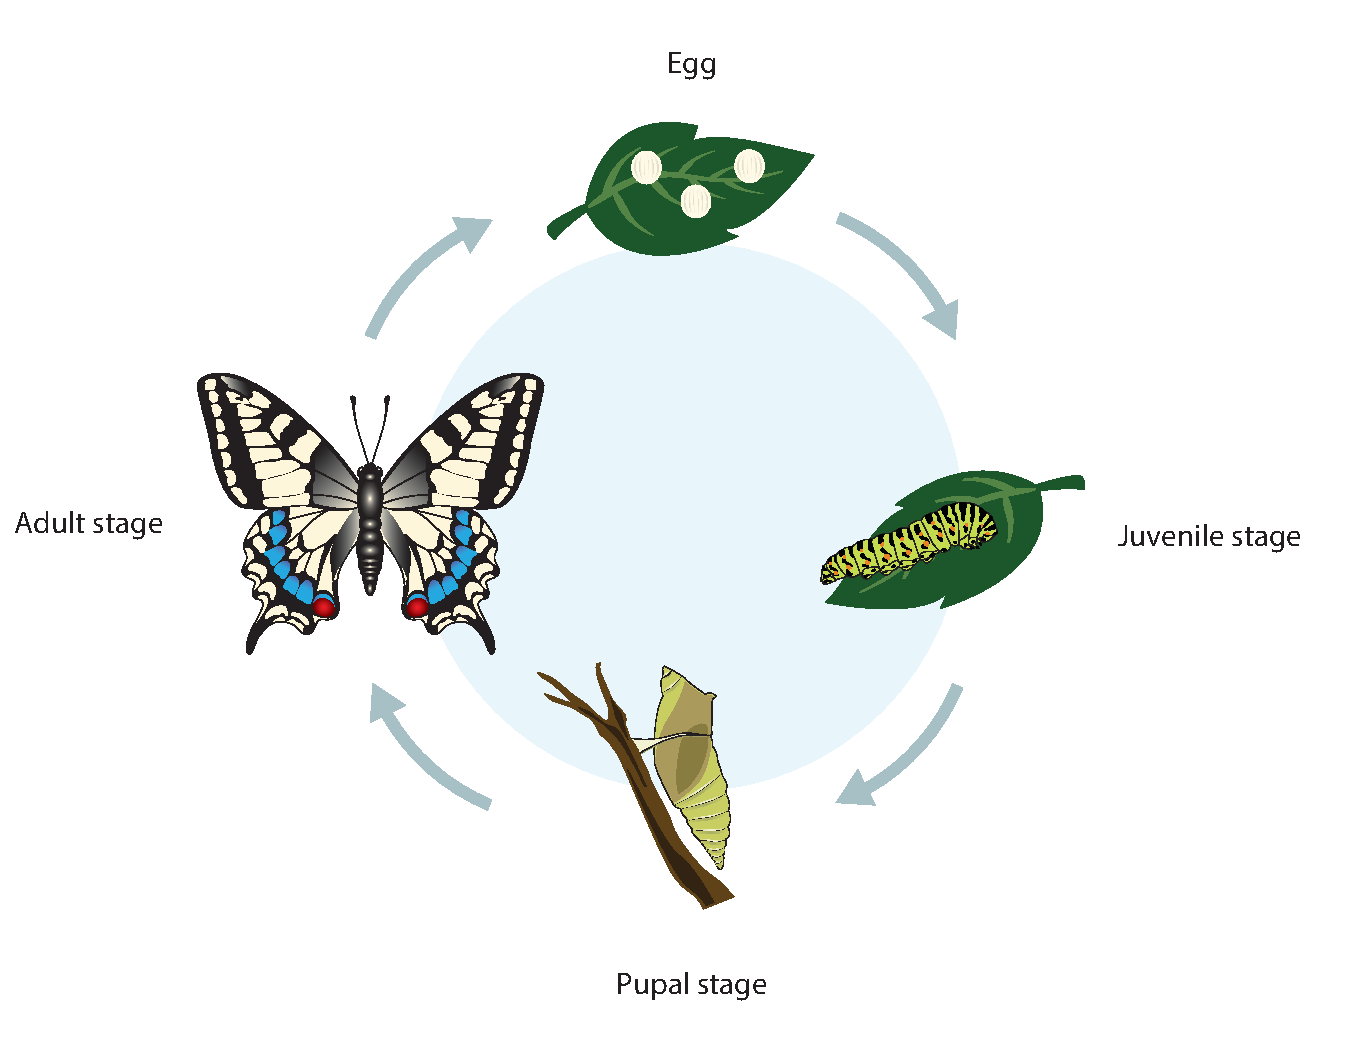
\includegraphics[width=0.9\textwidth]{papilo_machaon_life_cycle.pdf} 
\end{centering}
\end{figure}

The somatic mutation theory of ageing suggests that the gradual accumulation of somatic mutations leads to a decline in cellular function, which ultimately contributes to the ageing process \cite{Szilard1959-ru}. The theory also implies that shorter-lived species will have a higher somatic mutation rate than longer-lived species. Since somatic mutation rate is inversely proportional to the lifespan of species in mammals \cite{Cagan2022-yn}, I initially conjectured that somatic mutation rate would be higher in insects as most insects are short-lived \cite{Promislow2022-en}. I observed that mutation burden of insects was lower than what might have been expected from the somatic mutation theory of ageing and an alternative explanation was required for this observation (The DToL project sequences one sample per species and age of the sample is often not recorded. The calculation of somatic mutation rate requires multiple samples of different ages). 

As a disposable tissue that does not contribute to the germ line lineage, the human placenta has a higher mutation burden and chromosomal aberrations that are absent from the foetus \cite{Coorens2021-ct}. On the other hand, the human spermatogonia has the lowest somatic mutation rate \cite{Rahbari2016-ot}. Similarly, larval tissue in holometabola (a superorder of insects that undergoes complete metamorphosis) is a disposable tissue like the placenta that does not contribute to the development of the adult insect, and hence, larval tissue does not transmit genetic information to the next generation. During embryonic development, imaginal disc precursors separate from embryonic stem cells programmed for differentiation into larval tissue after the blastoderm stage and imaginal discs are set aside for further development into the structures of the adult insect during the pupal stage (An imaginal disc is a single layer of epithelial sheet that consists of 20 to 40 cells) \cite{Wieschaus1976}. Genitalia, for example, are derived from the medial disc in \textit{D. melanogaster} \cite{Bate1993}. Larva and adult insects are, therefore, derived from distinct embryonic lineage, aside from the histoblast cells that develop into the abdomen of the adult insect \cite{Bate1993}. Consequently, somatic mutations that were acquired in the larval stage should be absent in the adult insect and only the somatic mutations that arose during the first few cell divisions of embryonic development should be shared between the two tissues (Fig \ref{figure:lepidoptera-mutation-burden}). For instance, caterpillars, the larvae of butterflies and moths, primarily consume the leaves, stems and flowers of plants and the subsequent accumulation of chlorophyll pigment might be phototoxic to caterpillars. During photosynthesis, the photoexcitation of chlorophyll pigment is channelled to convert light energy into glucose and oxygen. In contrast, unregulated photoexcitation of chlorophyll pigment produces reactive oxygen species \cite{Foyer2018-in}. Hence, C>A somatic mutations associated with DNA damage by reactive oxygen species (SBS18 and SBS36) might the dominant somatic mutational process in caterpillars. 

\begin{figure}[h!]
\caption{Hypothetical changes in mutation burden with life cycle progression}
\label{figure:lepidoptera-mutation-burden}
\begin{centering}
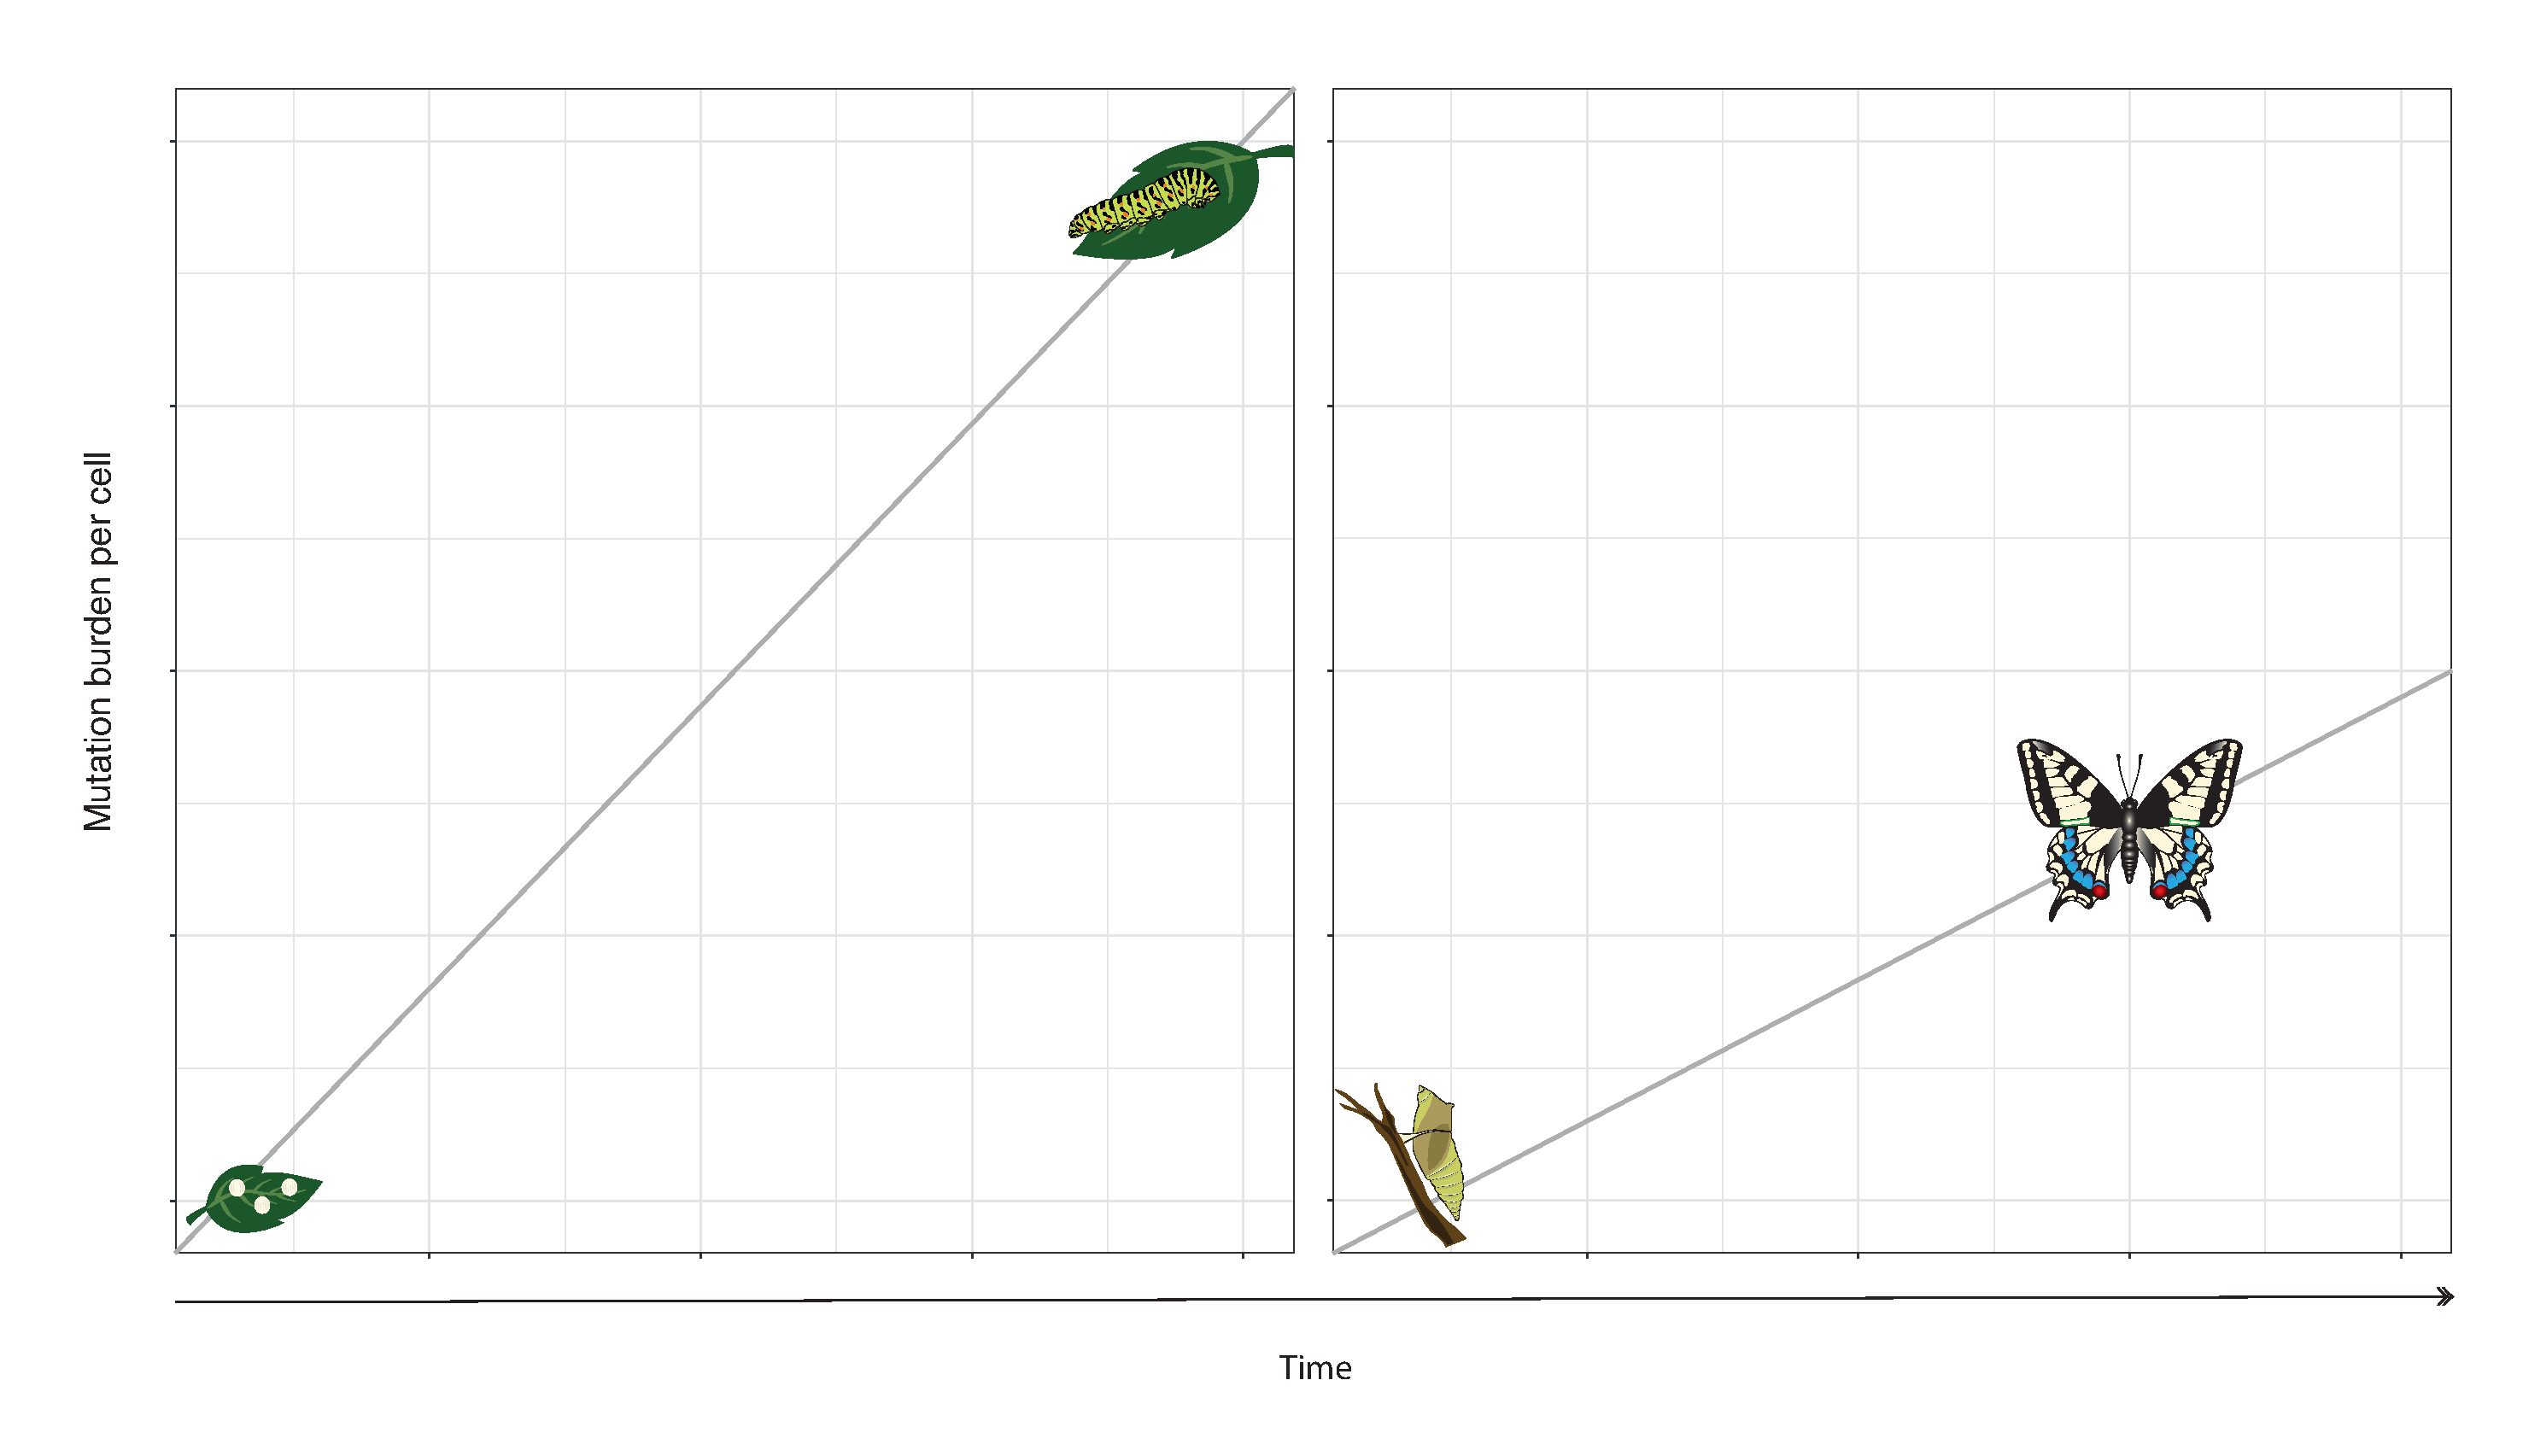
\includegraphics[width=\textwidth]{lepidoptera_mutation_burden.pdf} 
\end{centering}
\floatfoot{Larval tissue is hypothesised to have a higher somatic mutation rate than adult tissue. Somatic mutations acquired during the juvenile stage are not transmitted to the adult insect and a new somatic mutational process is operational in the adult tissue. }
\end{figure}

The life cycle and development of holometabolous insects corroborates the hypothesis that somatic mutations acquired during the larval stage are not shared with the adult insect. In addition, the hypothesis could be tested with insect species that exhibit sexual dimorphism in development. In certain insect species, females do not undergo metamorphosis, referred to as larviform female, while the males still undergo complete metamorphosis. CCS sequencing of both male and female samples with such sexual dimorphism could confirm whether somatic mutation rate is higher in the larval tissue. This experiment, however, does not address the question of why the mutation burden is low in adult insects despite the high cell division rate during metamorphosis. 

\section{Future directions}

In the imminent future, I conjecture that CCS library errors and inaccurate CCS BQ score estimation will be properly addressed and that the majority (>50\%) of CCS bases will have $\sim$Q90 base accuracy. Here, I discuss the potential opportunities following this development.

\subsection{Single-molecule real-time sequencing}

As discussed in chapter 1, CCS sequence throughput and sequencing cost per base is a function of the number of ZMWs and the read-of-insert length of the SMRTbell template. As demonstrated in chapter 2 and chapter 3, CCS base accuracy is a function of subread error rate and the number of subreads per CCS read, under the assumption that there are no new errors introduced during consensus sequence generation. Here, I make some informed predictions about the forthcoming advancements in the SMRT sequencing platform based on observations made in this PhD thesis.

I expect the number of ZMWs per SMRTcell to double every two to three years like how Moore’s Law predicts the number of transistors per chip to double every two years. As the number of ZMWs per SMRTcell increases exponentially, sequencing cost per base is expected to decrease exponentially as well (Fig \ref{figure:ccs_sequence_throughput}a). Moore’s law has continued for approximately $\sim$50 years and similar performance increases can be expected from SMRTcell as well. In addition, as CCS sequence throughput is directly proportional to CCS read length, the rate at which CCS sequence throughput increases could also exceed all our expectations due to the combined effect of parallel increases in both CCS read length and number of ZMWS per SMRTcell (Fig \ref{figure:ccs_sequence_throughput}b). 

\begin{figure}[h]
\caption{Exponential decay in CCS sequencing cost}\label{figure:ccs_sequence_throughput}
\begin{centering}
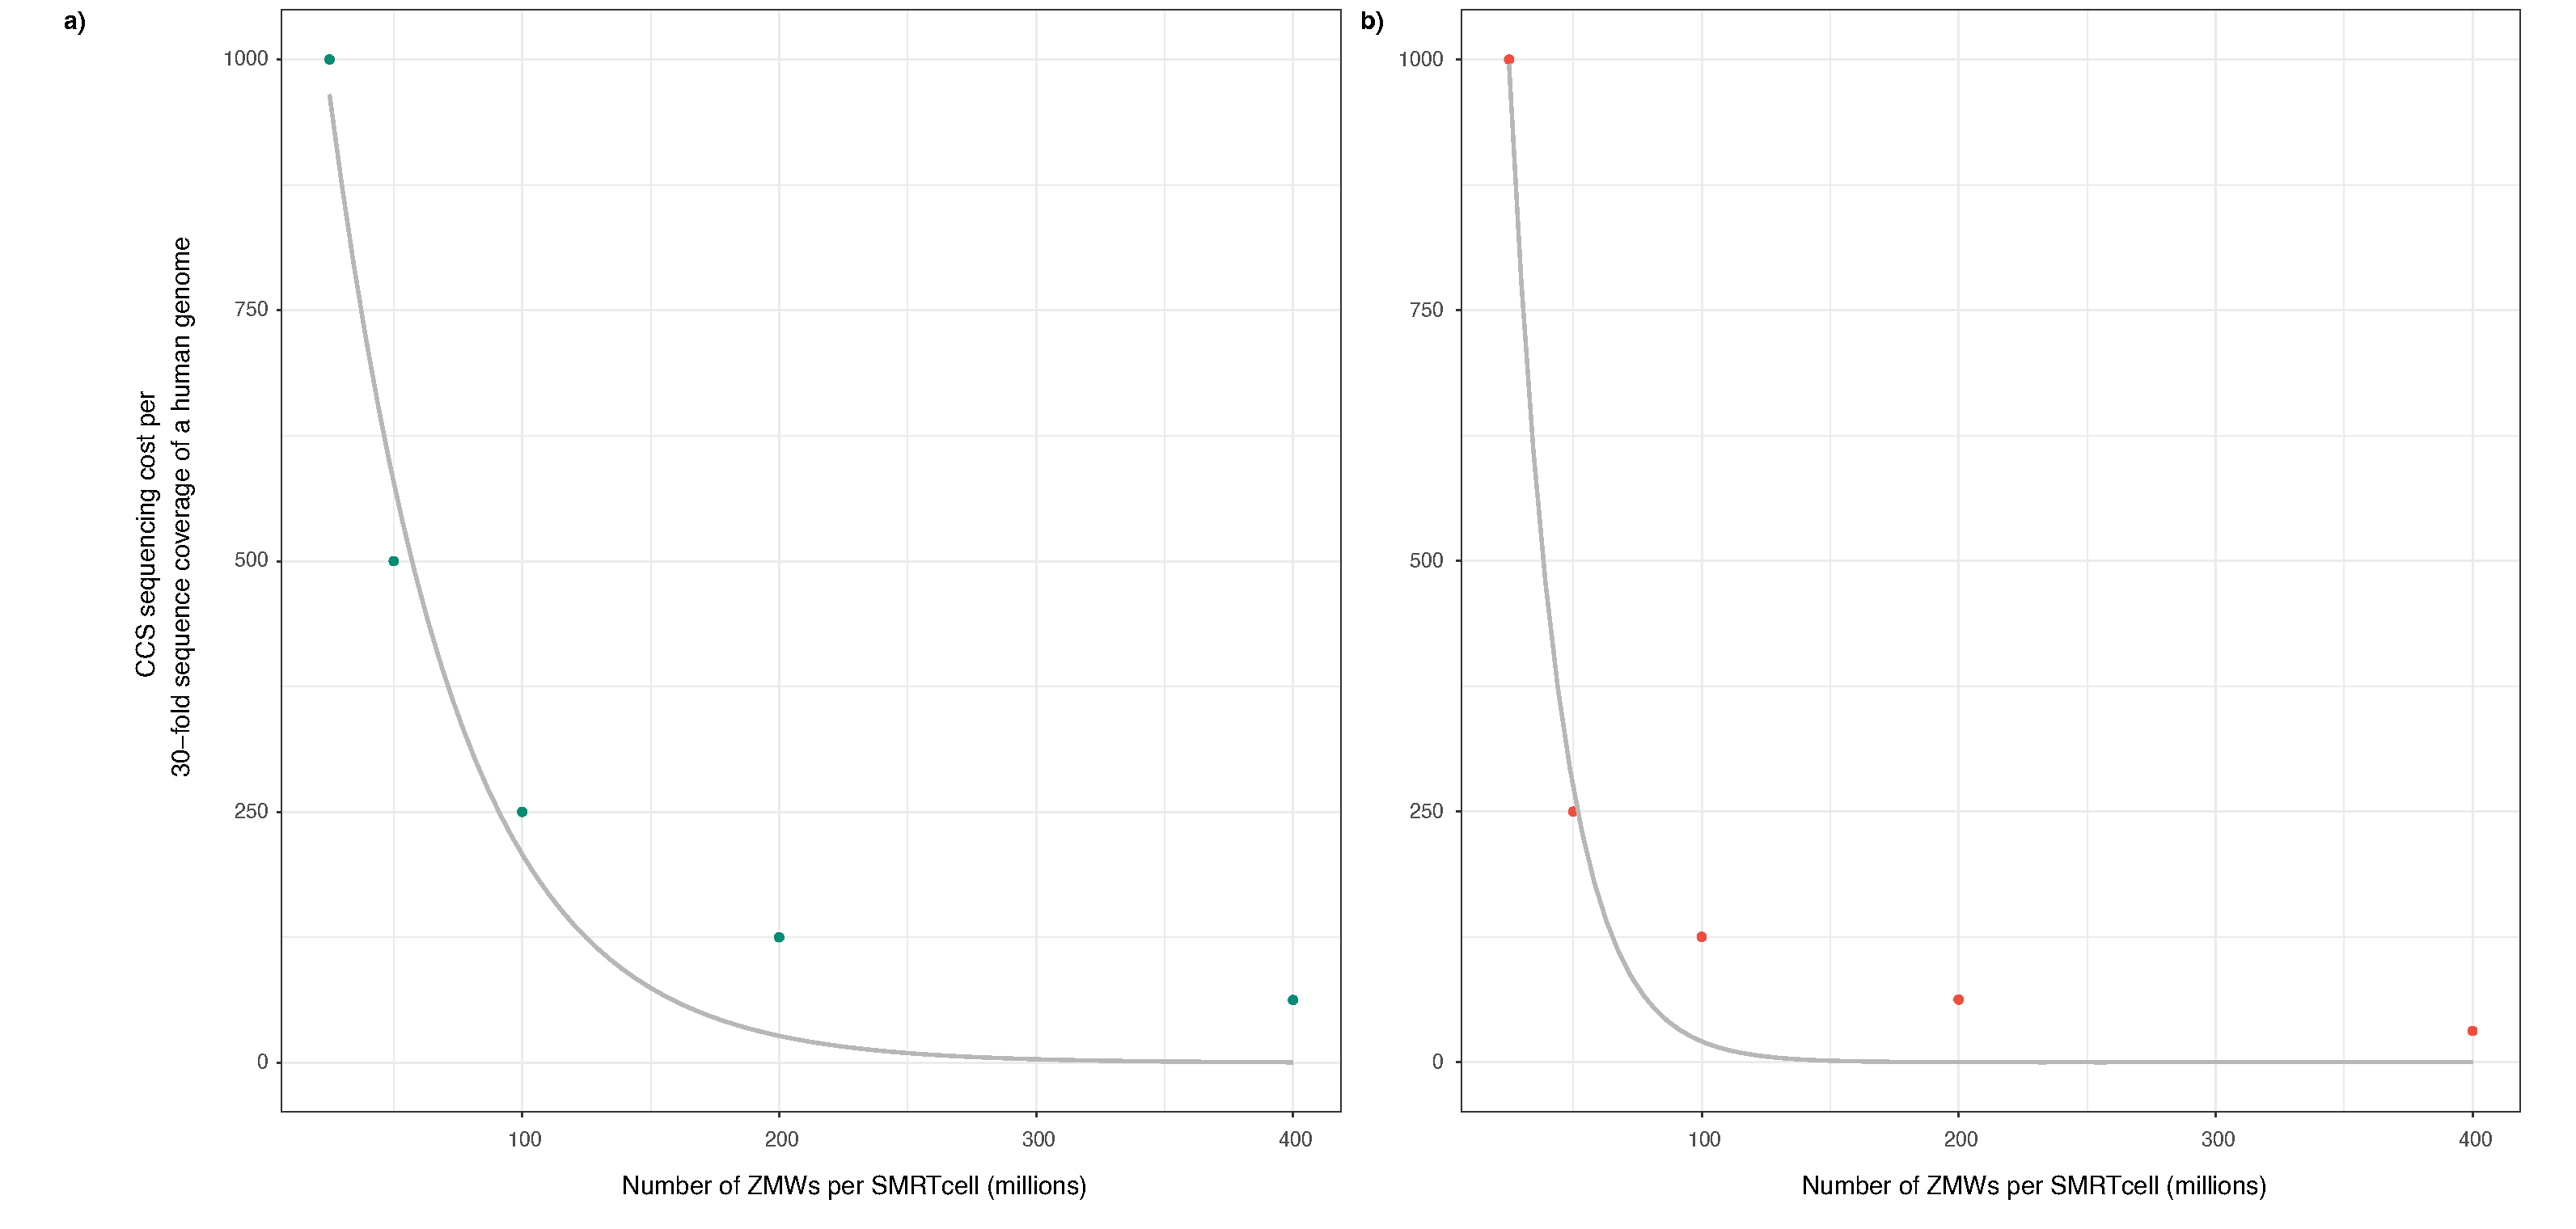
\includegraphics[width=\textwidth]{exponential_decay_in_ccs_sequencing_cost.pdf} \\ \smallskip
\end{centering}
\floatfoot{The graph starts with the current CCS sequencing cost for a 30-fold sequence coverage of a human genome using the Revio instrument, the latest SMRTcell with 25 million ZMWs and assumes that average CCS read length is around 20kb. \textbf{a)} Exponential decay in CCS sequencing cost with doubling in the number of ZMWs per SMRTcell. \textbf{b)} Exponential decay in CCS sequencing cost with doubling in both CCS read length and the number of ZMWs per SMRTcell.}
\end{figure}

To make accurate predictions about future technological advances, I must also consider Wright’s Law, a companion of Moore’s Law. Wright’s Law, also known as experience curve effect, states that for every cumulative doubling of units produced, costs will fall by a constant percentage. As discussed above, the rapid decrease in CCS sequencing costs will accelerate the adoption of CCS sequencing and when economies of scale are achieved, the positive flywheel effect will be unstoppable (Fig \ref{figure:flywheel}). 

\begin{figure}[h!]
\caption{Pacific Biosciences flywheel}
\label{figure:flywheel}
\begin{centering}
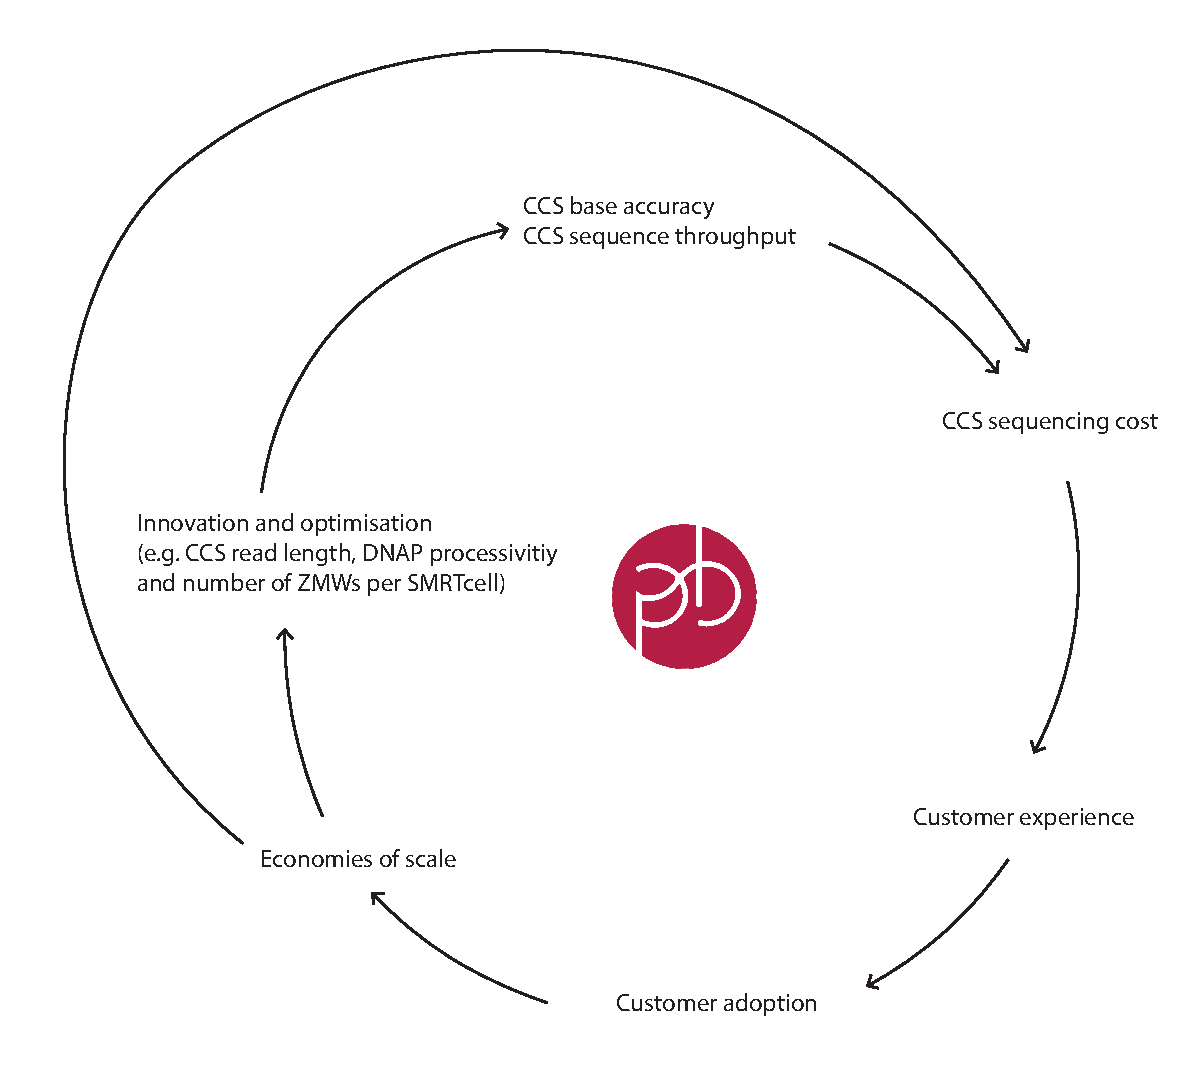
\includegraphics[width=0.75\textwidth]{pacbio_flywheel.pdf} \\ \smallskip
\end{centering}
\floatfoot{The flywheel symbolises how independent components act in concert to improve base accuracy, reduce sequencing cost and drive customer adoption}
\end{figure}


DNAP processivity, the rate at which DNAP synthesises a new strand of DNA, is another crucial factor that determines CCS base accuracy and sequence throughput. If the subread error rate is between 10\% and 15\%, CCS generation typically requires at least 10 subreads per CCS read to generate CCS bases with Q93 base accuracy. DNAP processivity determines the number of subreads per CCS read and hence, increasing DNAP processivity translates to increasing CCS read length. If, for example, DNAP processivity is doubled, CCS read length can also be doubled without sacrifices in base accuracy. DNAP’s biological limit, hence, will be the theoretical limit of CCS read length. In addition, DNAP replication error rate is not an obstacle to $\sim$Q90 CCS base generation at all trinucleotide sequence contexts as demonstrated in chapter 2. One interesting ramification of improved base accuracy is that pooled and non-barcoded samples can be sequenced together to detect common germline SNPs as lower sequence coverage is needed to call the germline mutations with confidence. In addition, as the number of somatic mutations increases linearly with sequence coverage, CCS sequence coverage will not determine the confidence with which germline mutations are detected, but the number of somatic mutations that are detected from the sample. 

In contrast, Illumina’s sequencing by synthesis approach has several disadvantages that limit improvements in read length and base accuracy. In each Illumina sequencing cycle, the rate at which a growing DNA becomes asynchronous with the rest of DNA fragments from the same cluster increases, resulting in a reduced signal-to-noise ratio as sequencing progresses \cite{Metzker2005-am}. This technical limitation places a ceiling on Illumina read length and is responsible for decline in per-base sequence quality towards the end of the read. In addition, CCS sequence throughput is a polynomial function with read length and number of ZMWs per SMRTcell as input while Illumina sequence throughput is a linear function with number of clusters per flow cell as the only input. Consequently, CCS sequencing possesses a greater potential for improving sequence throughput. Considering the fact that CCS reads enables \textit{de novo} assembly and simultaneous detection of haplotype phased somatic and germline mutations and epigenetic modifications, I believe that CCS sequencing will be the primary DNA sequencing method in clinics and research in the imminent future. 

\subsection{Strand-specific somatic mutation detection}

To date, somatic mutation detection in normal tissues and tumours with next-generation sequencing have focused on analysing sub-clonal or clonal somatic mutations that are fixed in a group of cells above the limit of detection threshold. Single-molecule resolution and strand-specific base modification somatic mutation detection has the potential to enhance our understanding of somatic mutagenesis.

As described in chapter 1, DNAP sequences both the forward and reverse strand of the SMRTbell template multiple times through rolling circle replication. The pbccs algorithm leverages the redundancies and complementary base pairing between the forward and reverse strand subreads to generate CCS reads. As demonstrated in chapter 2, CCS reads have sufficient base accuracy for single molecule somatic mutation detection and as described in a previous publication, single-molecule resolution 5mC detection is also possible from CCS DNAP kinetics \cite{Vong2019-bi, Tse2021-or}. The pbccs algorithm can also generate single-strand consensus sequence (SSCS) reads from the forward and reverse strand subreads. Strand-specific somatic mutation and base modification detection with SSCS reads presents an exciting opportunity to analyse somatic mutations from their beginning to their end. 

Somatic mutation is a three-step process: 1) DNA damage, mutation, or modification from endogenous or exogenous sources, 2) failure to detect and repair the DNA damage or mutation, and 3) fixation, persistence of DNA mutation in daughter cells through genetic drift or selection. In a population of DNA molecules, there will be a group of wild type DNA molecules, a group of DNA molecules with DNA damage, mutation or modification, a group of DNA molecules undergoing DNA damage repair and a group of DNA molecules with new somatic mutations (Fig \ref{figure:single-strand-specific-mutation}). 

\begin{figure}[htbp!]
\caption{SBS1 somatic mutational process}
\label{figure:single-strand-specific-mutation}
\begin{centering}
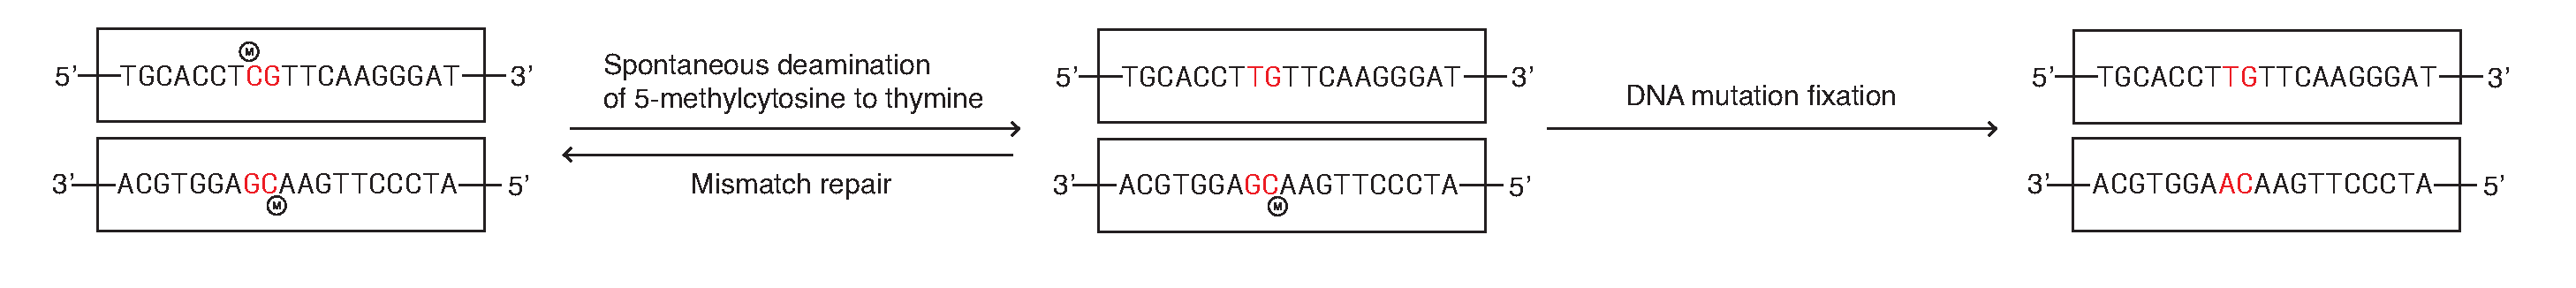
\includegraphics[width=\textwidth]{spontaneous_deamination.pdf} 
\end{centering}
\floatfoot{The figure illustrates how DNA mismatch resulting from spontaneous deamination of 5mC to thymine is repaired and how DNA mutation is fixed. The nucleotide bases in red highlights the methylated CG dinucleotide on both the forward and reverse strand of the DNA.}
\end{figure}

The DNA damage and repair process associated with SBS1 mutational signature, for example, is amenable to further qualitative and quantitative examination through this approach. The spontaneous deamination of 5mC to thymine results in a TG:GC mismatch and results in C>T somatic mutation at a CG dinucleotide if left unrepaired by the mismatch repair (MMR) pathway. If both strands of the double-stranded DNA molecule are sequenced, TG dinucleotide will be present on the strand where deamination has happened and GC dinucleotide with methylation will be present on the complementary strand. SSCS reads from SMRT sequencing enable the detection of TG:GC mismatches and associated hemi-methylation (Figure \ref{figure:single-strand-specific-mutation}). In addition, CCS reads allow the estimation of the number of methylated CG dinucleotides where deamination could have happened and the number of CG dinucleotides where somatic mutations have occurred. If the same tissue is sequenced at multiple different timepoints, the gain and loss of somatic mutations in the population can also be studied.

If successful, we will be able to measure the \textit{in vivo} deamination rate from the number of TG:GC mismatch and the number of GC dinucleotides, and compare it against the \textit{in vitro} deamination rate of $5.8\times10^{-13}$ per 5mC per second at 37°C \cite{Shen1994-of}. In addition, TG:GC mismatch repair efficiency and fidelity can also be measured under wild-type and mutant conditions. MutS$\alpha$, for example, is critical in recognising the TG:GC mismatch and initiating DNA damage repair. MutS$\alpha$ deficiency, therefore, elevates the number of C>T somatic mutations. Similarly, cross-examination of both SSCS and CCS reads and associated DNAP kinetics can also be used to better understand the C>T (SBS2) somatic mutations resulting from APOBEC-dependent deamination of cytosine to uracil.  

\subsection{Decomposition of a mutational signature}

Single-molecule resolution and strand-specific base modification somatic mutation detection, most importantly, creates an opportunity to gain greater insights into the dynamics of somatic mutational processes. Each somatic mutational process leaves a characteristic imprint to the genome and mutational signatures represent the probability that a specific somatic mutational process will produce a somatic mutation in a specific sequence context. Given a catalogue of somatic mutations from multiple samples, mutational signature analysis identifies the mutational signature in each sample and the contribution of each mutational signature to the mutation burden of the sample.

Since each mutational signature is a cumulative result of DNA damage, mutation or modification, failure to repair the DNA damage or mismatch, and persistence of the mutation in bulk tissue, each mutational signature can be re-defined as such (eq. \ref{eq:3})

\begin{align}
\begin{split} 
\alpha D \cdot \beta R \cdot \gamma F &\approx P_{i} \label{eq:3} \\
\alpha \begin{bmatrix}
    d^{1}_{1}  \\
    \vdots &  \\
    d^{96}_{1}  \\
\end{bmatrix} 
\beta \begin{bmatrix}
    r^{1}_{1} \\
    \vdots &  \\
    r^{96}_{1} \\
\end{bmatrix} 
\gamma \begin{bmatrix}
    f^{1}_{1}  \\
    \vdots &  \\
    f^{96}_{1}  \\
\end{bmatrix} &\approx
\begin{bmatrix}
    p^{1}_{1} \\
    \vdots \\
    p^{96}_{1} \\
\end{bmatrix}
\end{split}
\end{align}

where $D$ is the DNA damage matrix and each element is a probability that a specific sequence context will be damaged. $R$ is DNA damage repair matrix and each element is a probability that DNA damage in a specific sequence context will be repaired. $F$ is DNA mutation fixation matrix and each element is a probability that the mutation type will be fixed in the population. $\alpha$, $\beta$, $\gamma$ are scalar values that represent genetic and environmental factors that modulate the somatic mutational process. In addition, $R$ could be further decomposed into multiple subcomponents where each matrix represents a different DNA damage repair pathway specific to the DNA damage (eq. \ref{eq:4})

\begin{equation} \label{eq:4}
\alpha \begin{bmatrix}
    d^{1}_{1}  \\
    \vdots &  \\
    d^{96}_{1}  \\
\end{bmatrix} \
\beta \left[\begin{bmatrix}
    r^{1}_{i} \\
    \vdots &  \\
    r^{96}_{i} \\
\end{bmatrix} 
\begin{bmatrix}
    r^{1}_{i+1} \\
    \vdots &  \\
    r^{96}_{i+1} \\
\end{bmatrix} \ldots 
\begin{bmatrix}
    r^{1}_{n} \\
    \vdots &  \\
    r^{96}_{n} \\
\end{bmatrix}\right]
\gamma \begin{bmatrix}
    f^{1}_{1}  \\
    \vdots &  \\
    f^{96}_{1}  \\
\end{bmatrix} \approx
\begin{bmatrix}
    p^{1}_{1} \\
    \vdots \\
    p^{96}_{1} \\
\end{bmatrix}
\end{equation}

The decomposition of a mutational signature into their individual components and subcomponents should enable us to have a greater understanding of the nonlinear relationship between the components and the mechanisms underlying somatic mutagenesis.

\subsection{Gene conversion and crossover detection}

Here, I also hypothesise that CCS read length and base accuracy can be leveraged to detect gene conversion and crossover events generated during meiotic and mitotic recombination. Gene conversion and crossover (CO) (Fig \ref{figure:homologous-recombination}) arise from the non-reciprocal and reciprocal exchange of genetic material during double-strand break (DSB) repair through homologous recombination. Gene conversions are also referred to as non-crossovers (NCO), but gene conversions and crossovers are not mutually exclusive events \cite{Hunter2015-gk}. 

\begin{figure}[htbp!]
\caption{Gene conversion and crossover}
\label{figure:homologous-recombination}
\begin{centering}
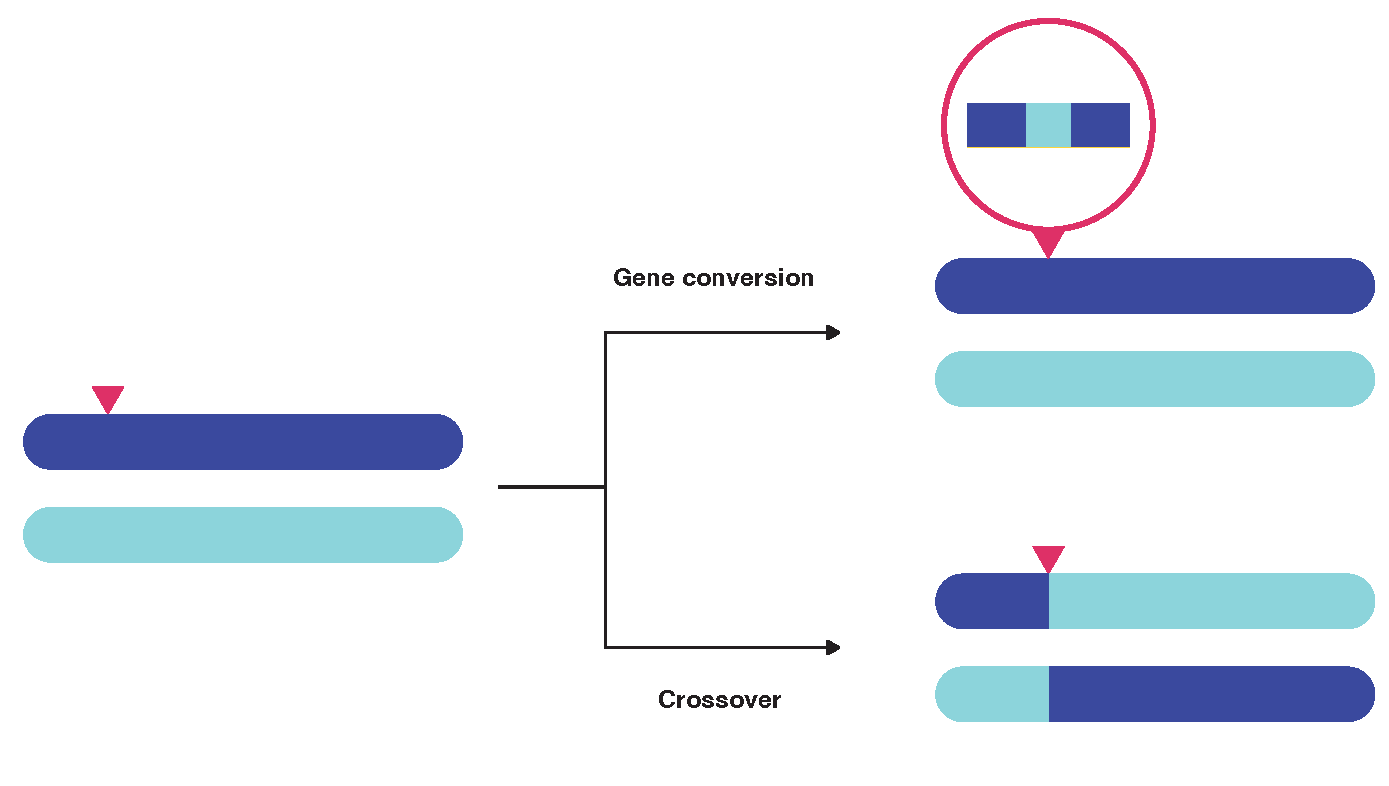
\includegraphics[width=\textwidth]{meiotic_recombination.pdf}
\end{centering}
\floatfoot{Red triangle indicates the DSB site. DSB can be repaired either as a gene conversion or as a crossover. Sister chromatids are not shown for simplification purposes.}
\end{figure}

In germ cells, meiotic recombination is an essential process that generates new combinations of alleles that serve as the foundation for adaptation and speciation through natural selection, an advantage for sexually reproducing organisms. In addition, the formation of at least one chiasma per pair of homologous chromosomes ensures proper segregation of chromosomes in anaphase I of meiosis. Improper chromosome segregation can result in aneuploid gametes with abnormal numbers of chromosomes. If DSB repair is not repaired in somatic cells, DNA damage response initiates programmed cell death. It is worth noting that DSB repair during meiotic recombination generates new allele combinations and contributes to genetic diversity, while DSB repair during mitotic recombination can result in the loss of heterozygosity (LOH). Furthermore, meiotic DSBs are deliberately introduced through the concerted action of PRDM9 and SPO11 to initiate meiotic recombination while mitotic DSBs are inadvertently generated from both endogenous (e.g. reactive oxygen species) and exogenous factors (e.g. ionising radiation).

A haplotype is a set of alleles that are inherited together in a single chromosome. Meiotic recombination yields a new haplotype with a new combination of alleles. Haplotype phasing, therefore, is not only essential for determining the original haplotype before meiotic recombination, but also the haplotype phase switch in individual gametes or in children after meiotic recombination. Trio-sequencing \cite{Kong2010-uk}, sperm-typing \cite{Webb2008-pw} and statistical methods leveraging the non-random association of alleles (linkage disequilibrium) \cite{Myers2005-ml} have been previously used to detect meiotic recombination products and each of these approaches have trade-offs in the resolution and the number of meiotic recombination event detected. Trio-sequencing approach, for example, detects one meiotic recombination per chromosome per child and enables the study of sex-specific meiotic recombination rate. In contrast, sperm-typing of a bulk sperm sample can detect multiple meiotic recombination events per target locus, but it requires prior knowledge of meiotic recombination hotspots. In addition, while statistical methods can generate high-resolution maps of recombination events from patterns of LD in the human population, they are unable to examine meiotic recombination events in an individual.

CCS sequencing of a bulk sperm sample should enable unbiased and genome-wide detection of meiotic recombination events. In addition, the number of detected events should be directly proportional to the sequence coverage as one chiasma per pair of homologous chromosomes is required for physical pairing and proper segregation of chromosomes. If a locus is a meiotic recombination hotspot, CCS sequencing of bulk sperm sample will yield three population of CCS reads: those derived from maternal haplotype, those derived from the paternal haplotype and those resulting from meiotic recombination and containing both maternal and paternal haplotypes. As discussed in chapter 2, CCS read length and base accuracy can be leveraged to phase hetSNPs and connect phased SNPs to construct a haplotype block. CCS haplotype, subsequently, can be determined from comparing CCS hetSNPs to that of the haplotype block. Similarly, CCS reads with both maternal and paternal haplotype can be identified from such a comparison. The length, and the number of phase transitions will also inform whether holliday junction (HJ) was resolved as a gene conversion or a crossover. It is worth noting that the resolution of the recombinant product detection and the number of loci from which recombinant products can be called from is higher in samples with greater heterozygosity. As detailed in chapter 3, many eukaryotic samples have a higher density of SNPs than human samples. In short, CCS base accuracy is used to not detect single molecule somatic mutations but detect single molecule phase transitions (Fig \ref{figure:phase-transitions}).

\begin{figure}[h!]
\caption{Gene conversion and crossover detection using CCS reads}
\label{figure:phase-transitions}
\begin{centering}
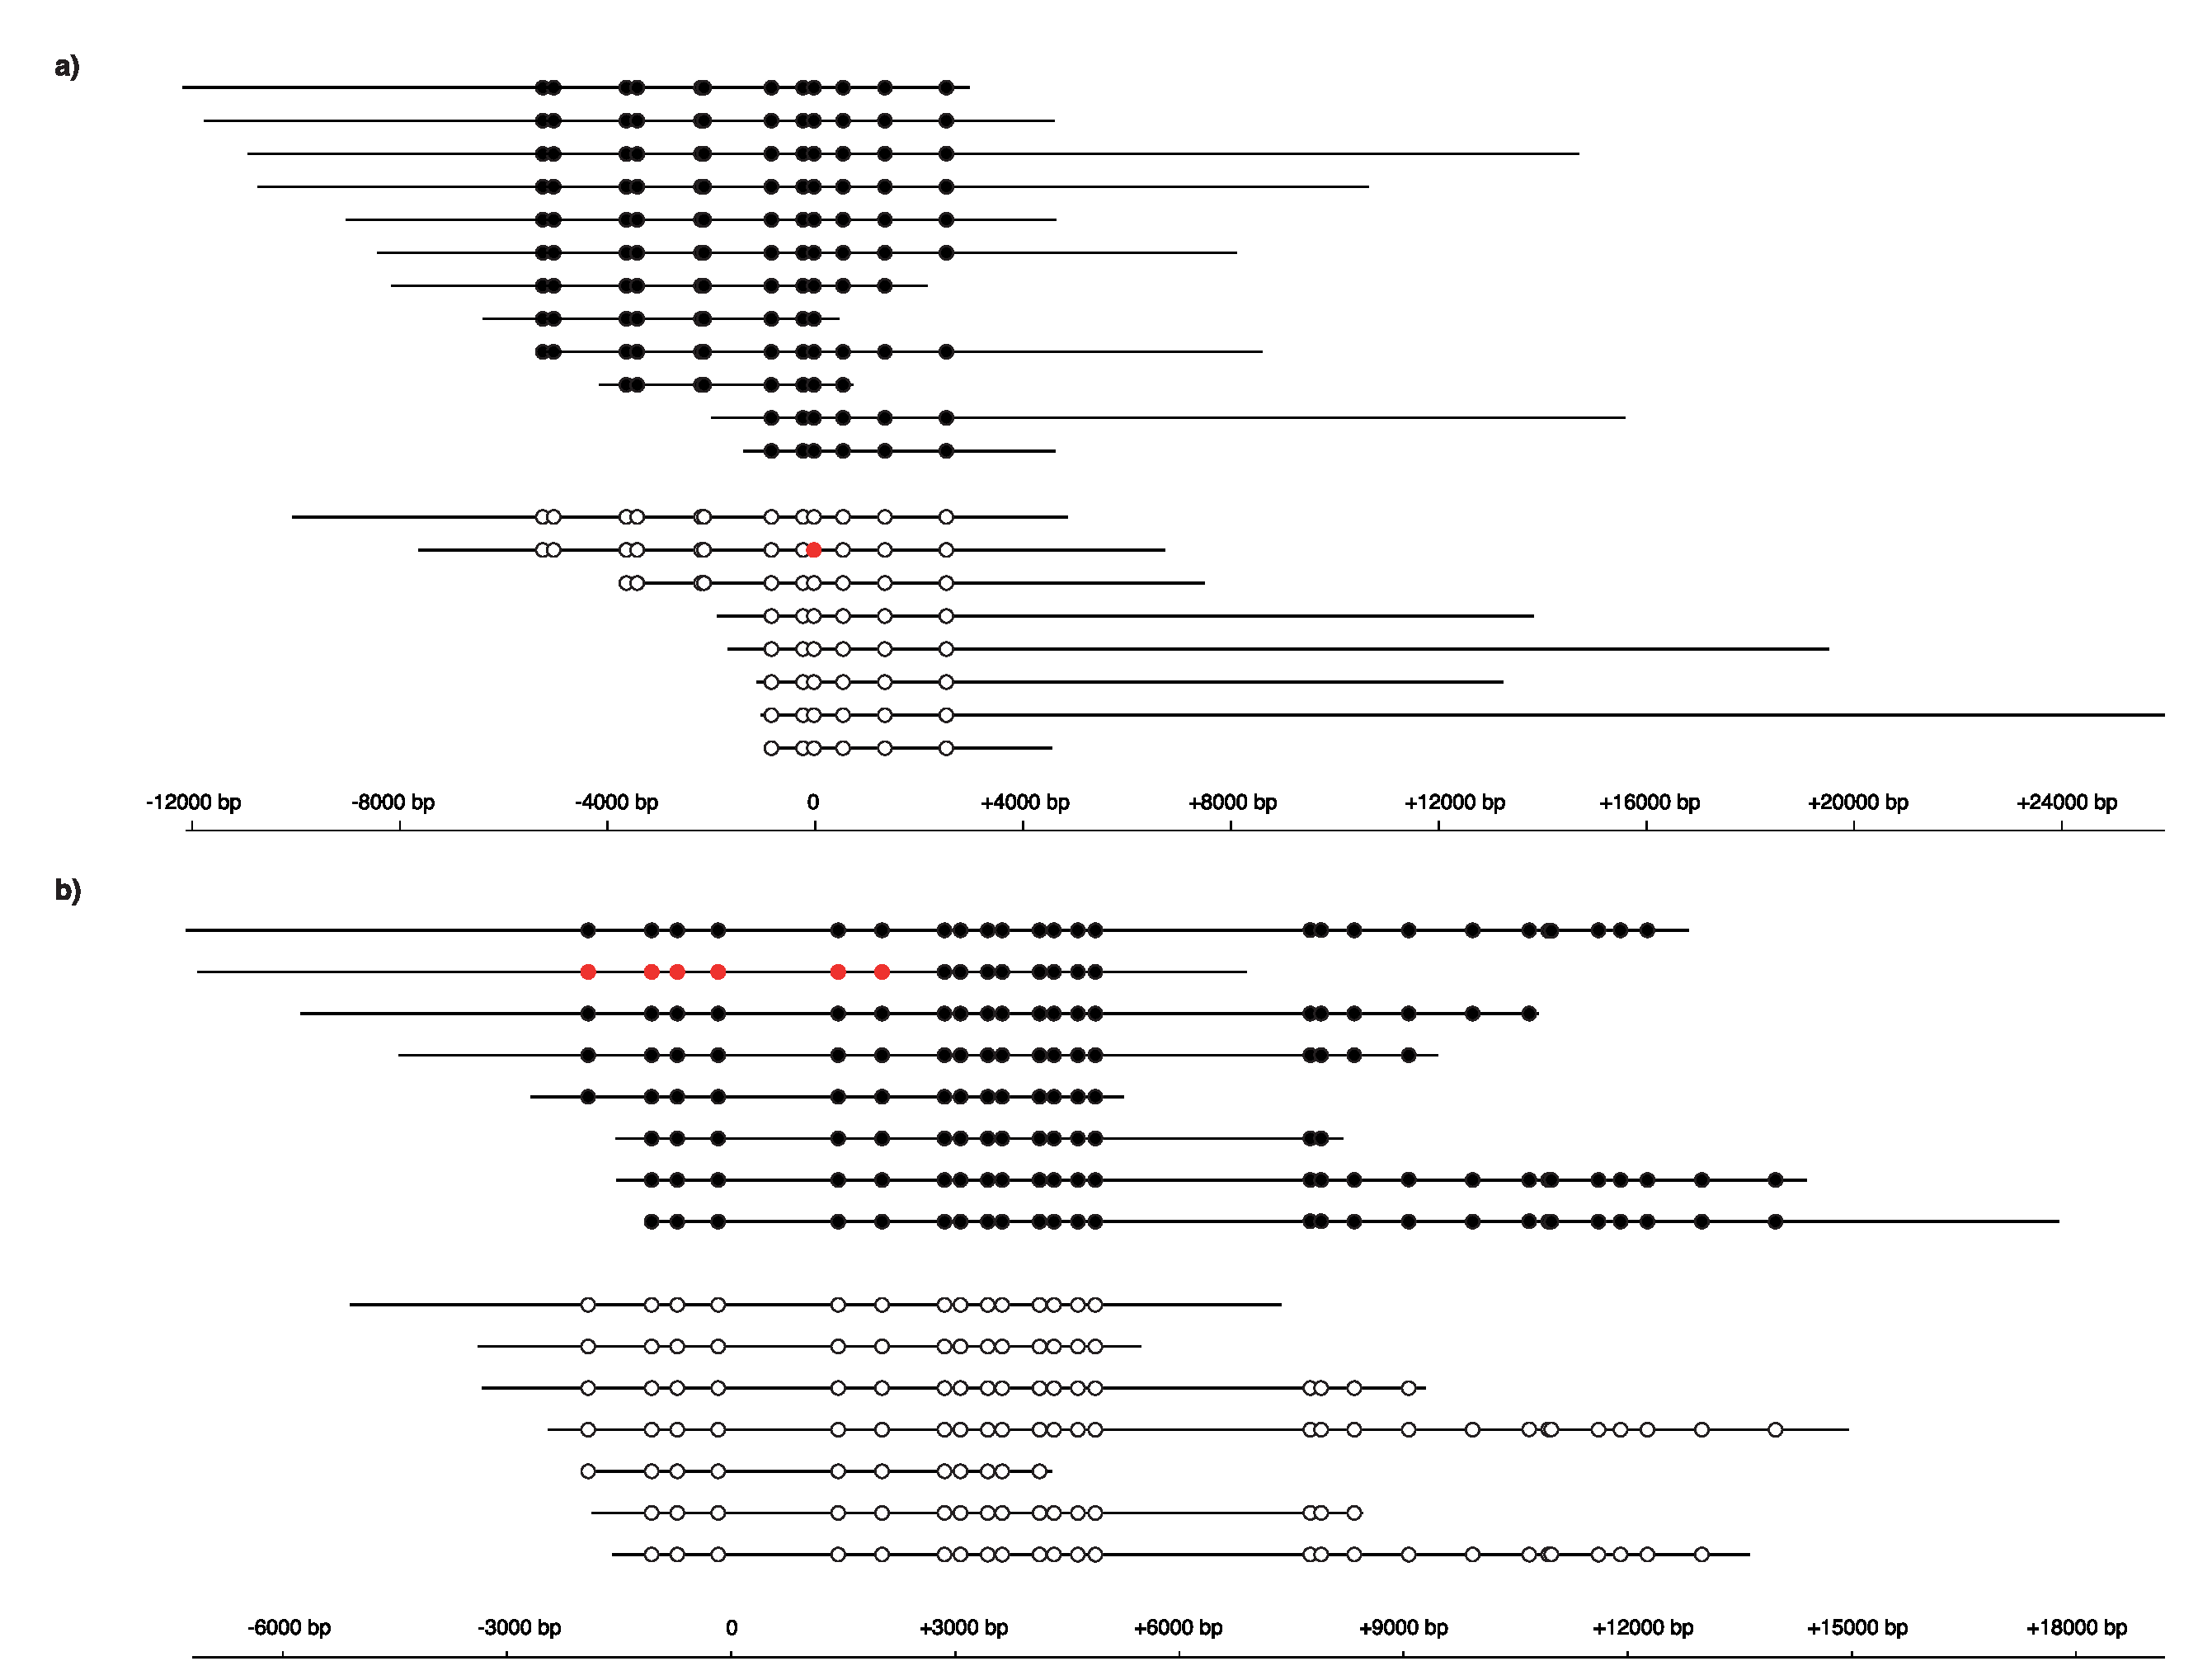
\includegraphics[width=\textwidth]{meiotic_recombination_detection.pdf} 
\end{centering}
\floatfoot{Each circle indicates a heterozygous SNP. A black circle indicates a reference allele, white circle indicates an alternative allele and red circle indicates a phase transition from reference allele to alternative allele and vice versa. CCS reads derived from the same haplotype have the same set of heterozygous SNPs. \textbf{a)} Gene conversion detection using CCS reads requires the phase transition to be flanked by wild type alleles of the haplotype. \textbf{b)} Crossover detection using CCS reads necessitates the phase transition to be continuous.}
\end{figure}

Our approach also has several advantages compared to existing methods and can greatly contribute to the body of research attempting to understand the hotspot conversion paradox \cite{Boulton1997-do}. \textit{De novo} mutations, for example, can be detected using himut and mutation burden across multiple samples of different ages can be used to define the germline mutation rate at scale in species where germline mutation rate is unknown. The hotspot conversion paradox stems from the fact that GC biased gene conversion leads to the loss of PRDM9 recognition sites and meiotic recombination hotspots. PRDM9 gene binds to a specific DNA sequence motif (CCNCCNTNNCCNC) \cite{Myers2008-st} and initiates meiotic recombination through the recruitment of SPO11 for programmed induction of double-strand breaks. The polymorphisms in the zinc finger array determine the exact DNA sequence motif and the PRDM9 binding site. The ability to determine the PRDM9 allele, identify PRDM9 \textit{de novo} mutations and detect gene conversion events using CCS reads should enable us to better understand how the rapid evolution of the PRDM9 gene resolves this paradox. 

The application of the above approach to somatic cells should enable the comprehensive characterisation of mitotic recombination and an assessment of how loss of heterozygosity contributes to oncogenesis in normal cells. Bloom syndrome patients, for example, with an autosomal recessive mutation in the BLM gene have increased risk of developing cancer \cite{Gruber2002-ck}. In addition, cross-examination of both meiotic and mitotic recombination products should elucidate the similarities and differences between these two processes and enhance our understanding of speciation and tumorigenesis. 

\section{Concluding remarks}

I conclude that factors that prevent the adoption of CCS sequencing are technical problems where solutions exist. As discussed in chapter 2, almost error-free CCS bases can be generated and as conjectured in this chapter, CCS sequencing cost and HMW DNA input requirement for CCS library preparation will no longer be a limitation to research. The exponential increase in the number of ZMWs per SMRTcell and the read-of-insert length will be the primary factors driving the increase in sequence throughput and decrease in per-base sequencing cost. The present sequencing methods necessitates a specific DNA input requirement to sequence the genome multiple times and thereby enable the detection of mutations with greater confidence despite the presence of sequencing errors. If DNAP processivity improves to enable CCS library preparation from longer read-of-insert and if CCS base accuracy improves to be error-free, only a single read will be required from each haplotype for germline and somatic mutation detection and epigenetic modification identification, drastically lowering the HMW DNA input requirements for CCS library preparation. I believe that we are witnessing a historic moment where error-free sequencing will be feasible at a fraction of current sequencing costs and where it will be possible to interrogate the genetic, epigenetic, and transcriptomic information of all forms of life.  










%%!TEX root = ../thesis.tex
%*******************************************************************************
%****************************** Third Chapter **********************************
%*******************************************************************************
\chapter{Mitotic Loss of Heterozygosity as an Oncogenic Mechanism}

% **************************** Define Graphics Path **************************
\ifpdf
    \graphicspath{{Chapter5/Figs/Raster/}{Chapter5/Figs/PDF/}{Chapter5/Figs/}}
\else
    \graphicspath{{Chapter5/Figs/Vector/}{Chapter5/Figs/}}
\fi

\section{Introduction}
\section{Materials \& Methods}
\section{Discussion}

%%!TEX root = ../thesis.tex
%*******************************************************************************
%****************************** Third Chapter **********************************
%*******************************************************************************
\chapter{Conclusion}

% **************************** Define Graphics Path **************************
\ifpdf
    \graphicspath{{Chapter5/Figs/Raster/}{Chapter5/Figs/PDF/}{Chapter5/Figs/}}
\else
    \graphicspath{{Chapter5/Figs/Vector/}{Chapter5/Figs/}}
\fi

\section{}
\section{}
\section{}

%\include{Chapter7/chapter7}



% ********************************** Back Matter *******************************
% Backmatter should be commented out, if you are using appendices after References
%\backmatter

% ********************************** Bibliography ******************************
\begin{spacing}{0.9}

% To use the conventional natbib style referencing
% Bibliography style previews: http://nodonn.tipido.net/bibstyle.php
% Reference styles: http://sites.stat.psu.edu/~surajit/present/bib.htm

%\bibliographystyle{apalike}
\bibliographystyle{unsrt} % Use for unsorted references  
%\bibliographystyle{plainnat} % use this to have URLs listed in References
\cleardoublepage
\bibliography{References/references} % Path to your References.bib file


% If you would like to use BibLaTeX for your references, pass `custombib' as
% an option in the document class. The location of 'reference.bib' should be
% specified in the preamble.tex file in the custombib section.
% Comment out the lines related to natbib above and uncomment the following line.

%\printbibliography[heading=bibintoc, title={References}]


\end{spacing}

% ********************************** Appendices ********************************

%% \begin{appendices} % Using appendices environment for more functunality
%% 
%% %!TEX root = ../thesis.tex
% ******************************* Thesis Appendix A ****************************


\newgeometry{hmargin=1cm,top=35mm,bottom=30mm}
\chapter{Samples from the Darwin Tree of Life project} 
\label{chapter:all_dtol_samples}

\begingroup
\footnotesize
\begin{centering}
\setlength{\LTright}{\LTleft}
%\begin{longtable}{c|c|c|c|c|c|>{\centering\arraybackslash}p{2cm}|c}
\begin{longtable}{l|l|l|l|l|l}
\label{} 
\textbf{DToL ID} & \makecell[{l}]{\textbf{Species} \\ \textbf{(Common name)}} & \textbf{Classification} & \textbf{\# of chr} & \textbf{Genome size} & \makecell[{l}]{\textbf{CCS} \\ \textbf{(read depth)}}  \\ \hline
bAccGen1 & \makecell[{l}]{\textit{Accipiter gentilis} \\ (Northern goshawk)} & Birds & 40 & 1.40 Gb & 36  \\ \hline
cmLunCruc20 & \makecell[{l}]{\textit{Lunularia cruciata} \\ (Crescent-cup liverwort)} & Non-vascular-plants & 9 & 565.88 Mb & 26  \\ \hline
daBalNigr1 & \makecell[{l}]{\textit{Ballota nigra} \\ (.)} & Dicots & 11 & 1.19 Gb & 32  \\ \hline
daMisOron1 & \makecell[{l}]{\textit{Misopates orontium} \\ (.)} & Dicots & 8 & 361.05 Mb & 36  \\ \hline
daPulDyse1 & \makecell[{l}]{\textit{Pulicaria dysenterica} \\ (.)} & Dicots & 9 & 833.27 Mb & 34  \\ \hline
daScuMino1 & \makecell[{l}]{\textit{Scutellaria minor} \\ (.)} & Dicots & 14 & 342.14 Mb & 63  \\ \hline
daSheArve1 & \makecell[{l}]{\textit{Sherardia arvensis} \\ (Field madder)} & Dicots & 11 & 441.90 Mb & 84  \\ \hline
daSolDulc1 & \makecell[{l}]{\textit{Solanum dulcamara} \\ (.)} & Dicots & 12 & 946.93 Mb & 30  \\ \hline
dcCheAlbu1 & \makecell[{l}]{\textit{Chenopodium album} \\ (White goosefoot)} & Dicots & 27 & 1.59 Gb & 30  \\ \hline
dcPolAvic1 & \makecell[{l}]{\textit{Polygonum aviculare} \\ (.)} & Dicots & 10 & 352.07 Mb & 77  \\ \hline
ddAraThal4 & \makecell[{l}]{\textit{Arabidopsis thaliana} \\ (.)} & Dicots & 5 & 138.84 Mb & 95  \\ \hline
ddMerAnnu1 & \makecell[{l}]{\textit{Mercurialis annua} \\ (.)} & Dicots & 0 & 453.17 Mb & 69  \\ \hline
dhQueRobu3 & \makecell[{l}]{\textit{Quercus robur} \\ (Common oak)} & Dicots & 12 & 789.74 Mb & 38  \\ \hline
drAilAlti1 & \makecell[{l}]{\textit{Ailanthus altissima} \\ (Tree of heaven)} & Dicots & 31 & 939.12 Mb & 51  \\ \hline
drBuxSemp1 & \makecell[{l}]{\textit{Buxus sempervirens} \\ (.)} & Dicots & 15 & 676.71 Mb & 0  \\ \hline
drChaAngu1 & \makecell[{l}]{\textit{Chamaenerion angustifolium} \\ (.)} & Dicots & 18 & 653.87 Mb & 47  \\ \hline
drFilUlma1 & \makecell[{l}]{\textit{Filipendula ulmaria} \\ (.)} & Dicots & 7 & 275.02 Mb & 52  \\ \hline
drGeuUrba1 & \makecell[{l}]{\textit{Geum urbanum} \\ (.)} & Dicots & 21 & 1.30 Gb & 29  \\ \hline
drHedHeli1 & \makecell[{l}]{\textit{Hedera helix} \\ (.)} & Dicots & 24 & 1.20 Gb & 40  \\ \hline
drHedHeli4 & \makecell[{l}]{\textit{.} \\ (.)} & Dicots & 24 & 1.20 Gb & 10  \\ \hline
drMalDome10 & \makecell[{l}]{\textit{Malus domestica} \\ (Apple)} & Dicots & 17 & 648.23 Mb & 34  \\ \hline
drMalDome11 & \makecell[{l}]{\textit{Malus domestica} \\ (Apple)} & Dicots & 17 & 652.81 Mb & 45  \\ \hline
drMalDome5 & \makecell[{l}]{\textit{Malus domestica} \\ (Apple)} & Dicots & 17 & 646.79 Mb & 29  \\ \hline
drMalDome58 & \makecell[{l}]{\textit{Malus domestica} \\ (Apple)} & Dicots & 17 & 642.68 Mb & 40  \\ \hline
drMalSylv7 & \makecell[{l}]{\textit{Malus sylvestris} \\ (.)} & Dicots & 17 & 640.99 Mb & 29  \\ \hline
drMedArab1 & \makecell[{l}]{\textit{Medicago arabica} \\ (.)} & Dicots & 8 & 515.51 Mb & 50  \\ \hline
drPotAnse1 & \makecell[{l}]{\textit{Potentilla anserina} \\ (.)} & Dicots & 7 & 237.42 Mb & 68  \\ \hline
drUrtUren1 & \makecell[{l}]{\textit{Urtica urens} \\ (.)} & Dicots & 12 & 340.11 Mb & 55  \\ \hline
eaMarGlac1 & \makecell[{l}]{\textit{Marthasterias glacialis} \\ (Spiny starfish)} & Echinoderms & 22 & 520.96 Mb & 48  \\ \hline
fBarBab1 & \makecell[{l}]{\textit{Barbus barbus} \\ (Barbel)} & Fish & 50 & 1.58 Gb & 48  \\ \hline
fBarBar1 & \makecell[{l}]{\textit{Barbatula barbatula} \\ (Stone loach)} & Fish & 25 & 617.66 Mb & 30  \\ \hline
fPhoGun1 & \makecell[{l}]{\textit{Pholis gunnellus} \\ (Rock gunnel)} & Fish & 24 & 588.70 Mb & 70  \\ \hline
fPlePla1 & \makecell[{l}]{\textit{Pleuronectes platessa} \\ (European plaice)} & Fish & 24 & 687.41 Mb & 31  \\ \hline
fSymMel2 & \makecell[{l}]{\textit{Symphodus melops} \\ (Corkwing wrasse)} & Fish & 23 & 636.37 Mb & 31  \\ \hline
fTauBub2 & \makecell[{l}]{\textit{Taurulus bubalis} \\ (Long-spined sea scorpion)} & Fish & 21 & 615.15 Mb & 38  \\ \hline
fTraTra1 & \makecell[{l}]{\textit{Trachurus trachurus} \\ (Atlantic horse mackerel)} & Fish & 24 & 820.16 Mb & 57  \\ \hline
gfAgaBisp1 & \makecell[{l}]{\textit{Agaricus bisporus} \\ (Cultivated mushroom)} & Fungi & 13 & 30.45 Mb & 23  \\ \hline
gfFlaVelt1 & \makecell[{l}]{\textit{Flammulina velutipes} \\ (Velvet shank)} & Fungi & 12 & 37.43 Mb & 121  \\ \hline
gfLaeSulp1 & \makecell[{l}]{\textit{Laetiporus sulphureus} \\ (Chicken of the woods)} & Fungi & 14 & 37.41 Mb & 109  \\ \hline
gfPleOstr1 & \makecell[{l}]{\textit{Pleurotus ostreatus} \\ (Oyster mushroom)} & Fungi & 12 & 40.63 Mb & 72  \\ \hline
grTriPseu1 & \makecell[{l}]{\textit{Trichoderma pseudokoningii} \\ (.)} & Fungi & 7 & 32.98 Mb & 286  \\ \hline
gsMetZobe1 & \makecell[{l}]{\textit{Metschnikowia zobellii} \\ ((a marine yeast))} & Fungi & 5 & 13.65 Mb & 1345  \\ \hline
gzMucPiri1 & \makecell[{l}]{\textit{Mucor piriformis} \\ (.)} & Fungi & 6 & 34.94 Mb & 89  \\ \hline
icAdaBipu1 & \makecell[{l}]{\textit{Adalia bipunctata} \\ (2-spot ladybird)} & \makecell[{l}]{Insects \\ (Coleoptera)} & 11 & 475.29 Mb & 50  \\ \hline
icAgoFuli1 & \makecell[{l}]{\textit{Agonum fuliginosum} \\ (.)} & \makecell[{l}]{Insects \\ (Coleoptera)} & 19 & 695.91 Mb & 31  \\ \hline
icAgrCyan1 & \makecell[{l}]{\textit{Agrilus cyanescens} \\ (.)} & \makecell[{l}]{Insects \\ (Coleoptera)} & 10 & 292.35 Mb & 56  \\ \hline
icAnaMacu3 & \makecell[{l}]{\textit{Anaspis maculata} \\ (.)} & \makecell[{l}]{Insects \\ (Coleoptera)} & 8 & 757.84 Mb & 31  \\ \hline
icApoCory1 & \makecell[{l}]{\textit{Apoderus coryli} \\ (Hazel leaf-roller)} & \makecell[{l}]{Insects \\ (Coleoptera)} & 20 & 428.08 Mb & 60  \\ \hline
icCanRufa1 & \makecell[{l}]{\textit{Cantharis rufa} \\ (.)} & \makecell[{l}]{Insects \\ (Coleoptera)} & 7 & 355.33 Mb & 17  \\ \hline
icCanRust1 & \makecell[{l}]{\textit{Cantharis rustica} \\ (Sailor beetle)} & \makecell[{l}]{Insects \\ (Coleoptera)} & 7 & 445.94 Mb & 45  \\ \hline
icCanRust3 & \makecell[{l}]{\textit{.} \\ (.)} & \makecell[{l}]{Insects \\ (Coleoptera)} & 7 & 445.94 Mb & 53  \\ \hline
icCetAura1 & \makecell[{l}]{\textit{Cetonia aurata} \\ (.)} & \makecell[{l}]{Insects \\ (Coleoptera)} & 11 & 479.65 Mb & 58  \\ \hline
icCocSept1 & \makecell[{l}]{\textit{Coccinella septempunctata} \\ (Seven-spotted ladybird)} & \makecell[{l}]{Insects \\ (Coleoptera)} & 10 & 398.87 Mb & 84  \\ \hline
icCryMora2 & \makecell[{l}]{\textit{Cryptocephalus moraei} \\ (.)} & \makecell[{l}]{Insects \\ (Coleoptera)} & 15 & 500.56 Mb & 39  \\ \hline
icElmAene2 & \makecell[{l}]{\textit{Elmis aenea} \\ (Riffle beetle)} & \makecell[{l}]{Insects \\ (Coleoptera)} & 9 & 516.52 Mb & 32  \\ \hline
icHalSede1 & \makecell[{l}]{\textit{Halyzia sedecimguttata} \\ (Orange ladybird)} & \makecell[{l}]{Insects \\ (Coleoptera)} & 10 & 911.60 Mb & 55  \\ \hline
icHarAxyr1 & \makecell[{l}]{\textit{Harmonia axyridis} \\ (Harlequin)} & \makecell[{l}]{Insects \\ (Coleoptera)} & 8 & 425.54 Mb & 59  \\ \hline
icLagHirt1 & \makecell[{l}]{\textit{Lagria hirta} \\ (.)} & \makecell[{l}]{Insects \\ (Coleoptera)} & 12 & 336.78 Mb & 76  \\ \hline
icLepMacu1 & \makecell[{l}]{\textit{Rutpela maculata} \\ (.)} & \makecell[{l}]{Insects \\ (Coleoptera)} & 10 & 2.02 Gb & 31  \\ \hline
icLocCapr1 & \makecell[{l}]{\textit{Lochmaea capreae} \\ (Willow leaf beetle)} & \makecell[{l}]{Insects \\ (Coleoptera)} & 17 & 534.69 Mb & 51  \\ \hline
icLocCrat2 & \makecell[{l}]{\textit{Lochmaea crataegi} \\ (Hawthorn leaf beetle)} & \makecell[{l}]{Insects \\ (Coleoptera)} & 16 & 891.30 Mb & 33  \\ \hline
icMalBipu1 & \makecell[{l}]{\textit{Malachius bipustulatus} \\ (Common malachite beetle)} & \makecell[{l}]{Insects \\ (Coleoptera)} & 10 & 544.26 Mb & 34  \\ \hline
icMelMelo1 & \makecell[{l}]{\textit{Melolontha melolontha} \\ (Cockchafer)} & \makecell[{l}]{Insects \\ (Coleoptera)} & 10 & 1.66 Gb & 34  \\ \hline
icNebBrev1 & \makecell[{l}]{\textit{Nebria brevicollis} \\ (.)} & \makecell[{l}]{Insects \\ (Coleoptera)} & 15 & 241.93 Mb & 99  \\ \hline
icNebSali1 & \makecell[{l}]{\textit{Nebria salina} \\ (.)} & \makecell[{l}]{Insects \\ (Coleoptera)} & 21 & 256.64 Mb & 76  \\ \hline
icOcyOlen1 & \makecell[{l}]{\textit{Ocypus olens} \\ (Devil's coach horse)} & \makecell[{l}]{Insects \\ (Coleoptera)} & 19 & 1.08 Gb & 37  \\ \hline
icPhiCogn1 & \makecell[{l}]{\textit{Philonthus cognatus} \\ (Rove beetle)} & \makecell[{l}]{Insects \\ (Coleoptera)} & 12 & 1.03 Gb & 29  \\ \hline
icPodAlpi1 & \makecell[{l}]{\textit{Podabrus alpinus} \\ (.)} & \makecell[{l}]{Insects \\ (Coleoptera)} & 7 & 777.25 Mb & 32  \\ \hline
icPolCerv1 & \makecell[{l}]{\textit{Polydrusus cervinus} \\ (.)} & \makecell[{l}]{Insects \\ (Coleoptera)} & 11 & 713.37 Mb & 39  \\ \hline
icPteMadi1 & \makecell[{l}]{\textit{Pterostichus madidus} \\ (Black clock beetle)} & \makecell[{l}]{Insects \\ (Coleoptera)} & 19 & 705.16 Mb & 35  \\ \hline
icPteNige1 & \makecell[{l}]{\textit{Pterostichus niger} \\ (.)} & \makecell[{l}]{Insects \\ (Coleoptera)} & 19 & 674.10 Mb & 4  \\ \hline
icPyrSerr1 & \makecell[{l}]{\textit{Pyrochroa serraticornis} \\ (Red-headed cardinal beetle)} & \makecell[{l}]{Insects \\ (Coleoptera)} & 10 & 249.41 Mb & 32  \\ \hline
icRhaFulv1 & \makecell[{l}]{\textit{Rhagonycha fulva} \\ (Common red soldier beetle)} & \makecell[{l}]{Insects \\ (Coleoptera)} & 7 & 424.68 Mb & 37  \\ \hline
icSilAtra2 & \makecell[{l}]{\textit{Phosphuga atrata} \\ (Black snail beetle)} & \makecell[{l}]{Insects \\ (Coleoptera)} & 18 & 1.20 Gb & 30  \\ \hline
idAcrOrbc1 & \makecell[{l}]{\textit{Acrocera orbiculus} \\ (Top-horned hunchback)} & \makecell[{l}]{Insects \\ (Diptera)} & 5 & 221.03 Mb & 105  \\ \hline
idBelPand1 & \makecell[{l}]{\textit{Bellardia pandia} \\ (Bisetose emerald-bottle)} & \makecell[{l}]{Insects \\ (Diptera)} & 6 & 617.21 Mb & 54  \\ \hline
idBerChal2 & \makecell[{l}]{\textit{Beris chalybata} \\ (Yellow-legged black legionnaire)} & \makecell[{l}]{Insects \\ (Diptera)} & 6 & 541.87 Mb & 42  \\ \hline
idBibMarc1 & \makecell[{l}]{\textit{Bibio marci} \\ (St. mark's fly)} & \makecell[{l}]{Insects \\ (Diptera)} & 6 & 340.02 Mb & 52  \\ \hline
idBleFall4 & \makecell[{l}]{\textit{Blera fallax} \\ (Pine hoverfly)} & \makecell[{l}]{Insects \\ (Diptera)} & 7 & 461.84 Mb & 56  \\ \hline
idBomDisc1 & \makecell[{l}]{\textit{Bombylius discolor} \\ (Dotted bee fly)} & \makecell[{l}]{Insects \\ (Diptera)} & 6 & 279.84 Mb & 26  \\ \hline
idBomMajo1 & \makecell[{l}]{\textit{Bombylius major} \\ (Dark edged bee fly)} & \makecell[{l}]{Insects \\ (Diptera)} & 7 & 304.33 Mb & 66  \\ \hline
idCheImpr3 & \makecell[{l}]{\textit{Cheilosia impressa} \\ (.)} & \makecell[{l}]{Insects \\ (Diptera)} & 6 & 394.97 Mb & 38  \\ \hline
idChePaga1 & \makecell[{l}]{\textit{Cheilosia pagana} \\ (Parsley cheilosia)} & \makecell[{l}]{Insects \\ (Diptera)} & 6 & 354.13 Mb & 52  \\ \hline
idCheVern2 & \makecell[{l}]{\textit{Cheilosia vernalis} \\ (Yarrow cheilosia)} & \makecell[{l}]{Insects \\ (Diptera)} & 6 & 441.64 Mb & 68  \\ \hline
idCheVulp2 & \makecell[{l}]{\textit{Cheilosia vulpina} \\ (Large burdock cheilosia)} & \makecell[{l}]{Insects \\ (Diptera)} & 6 & 405.38 Mb & 53  \\ \hline
idChrBici1 & \makecell[{l}]{\textit{Chrysotoxum bicinctum} \\ (Two-banded wasp hoverfly)} & \makecell[{l}]{Insects \\ (Diptera)} & 5 & 912.94 Mb & 29  \\ \hline
idCluTigr1 & \makecell[{l}]{\textit{Clusia tigrina} \\ (.)} & \makecell[{l}]{Insects \\ (Diptera)} & 5 & 1.22 Gb & 29  \\ \hline
idCoePili4 & \makecell[{l}]{\textit{Coelopa pilipes} \\ (.)} & \makecell[{l}]{Insects \\ (Diptera)} & 7 & 262.97 Mb & 75  \\ \hline
idCorMarg1 & \makecell[{l}]{\textit{Coremacera marginata} \\ (.)} & \makecell[{l}]{Insects \\ (Diptera)} & 6 & 979.68 Mb & 26  \\ \hline
idCriBerb1 & \makecell[{l}]{\textit{Criorhina berberina} \\ (Dimorphic bear hoverfly)} & \makecell[{l}]{Insects \\ (Diptera)} & 4 & 410.47 Mb & 35  \\ \hline
idEpiGros1 & \makecell[{l}]{\textit{Epistrophe grossulariae} \\ (Broad-banded epistrophe)} & \makecell[{l}]{Insects \\ (Diptera)} & 5 & 556.61 Mb & 29  \\ \hline
idEpiSucc1 & \makecell[{l}]{\textit{Epicampocera succincta} \\ (.)} & \makecell[{l}]{Insects \\ (Diptera)} & 7 & 398.13 Mb & 48  \\ \hline
idEriArbu1 & \makecell[{l}]{\textit{Eristalis arbustorum} \\ (Plane-faced dronefly)} & \makecell[{l}]{Insects \\ (Diptera)} & 6 & 451.04 Mb & 20  \\ \hline
idEriPert2 & \makecell[{l}]{\textit{Eristalis pertinax} \\ (Tapered dronefly)} & \makecell[{l}]{Insects \\ (Diptera)} & 7 & 482.09 Mb & 29  \\ \hline
idEriTena2 & \makecell[{l}]{\textit{Eristalis tenax} \\ (The dronefly)} & \makecell[{l}]{Insects \\ (Diptera)} & 6 & 487.02 Mb & 38  \\ \hline
idEupLati1 & \makecell[{l}]{\textit{Eupeodes latifasciatus} \\ (Meadow field syrph)} & \makecell[{l}]{Insects \\ (Diptera)} & 4 & 846.36 Mb & 28  \\ \hline
idGymRotn1 & \makecell[{l}]{\textit{Gymnosoma rotundatum} \\ (.)} & \makecell[{l}]{Insects \\ (Diptera)} & 6 & 780.52 Mb & 31  \\ \hline
idLypDubi1 & \makecell[{l}]{\textit{Lypha dubia} \\ (.)} & \makecell[{l}]{Insects \\ (Diptera)} & 6 & 645.06 Mb & 25  \\ \hline
idMacAtri3 & \makecell[{l}]{\textit{Machimus atricapillus} \\ (.)} & \makecell[{l}]{Insects \\ (Diptera)} & 6 & 268.64 Mb & 43  \\ \hline
idMelAuri2 & \makecell[{l}]{\textit{Meliscaeva auricollis} \\ (Spotted meliscaeva)} & \makecell[{l}]{Insects \\ (Diptera)} & 5 & 385.17 Mb & 36  \\ \hline
idMelMell2 & \makecell[{l}]{\textit{Melanostoma mellinum} \\ (Dumpy grass hoverfly)} & \makecell[{l}]{Insects \\ (Diptera)} & 5 & 731.04 Mb & 27  \\ \hline
idMyaFlor2 & \makecell[{l}]{\textit{Myathropa florea} \\ (Batman hoverfly)} & \makecell[{l}]{Insects \\ (Diptera)} & 6 & 485.10 Mb & 29  \\ \hline
idMyoTess1 & \makecell[{l}]{\textit{Myopa tessellatipennis} \\ (.)} & \makecell[{l}]{Insects \\ (Diptera)} & 4 & 249.28 Mb & 79  \\ \hline
idNeoCyan1 & \makecell[{l}]{\textit{Neoitamus cyanurus} \\ (Common awl robberfly)} & \makecell[{l}]{Insects \\ (Diptera)} & 10 & 365.51 Mb & 61  \\ \hline
idNepScut1 & \makecell[{l}]{\textit{Nephrocerus scutellatus} \\ (.)} & \makecell[{l}]{Insects \\ (Diptera)} & 6 & 613.39 Mb & 41  \\ \hline
idNowFero1 & \makecell[{l}]{\textit{Nowickia ferox} \\ (.)} & \makecell[{l}]{Insects \\ (Diptera)} & 6 & 670.72 Mb & 41  \\ \hline
idPheCory1 & \makecell[{l}]{\textit{Pherbina coryleti} \\ (.)} & \makecell[{l}]{Insects \\ (Diptera)} & 6 & 862.97 Mb & 24  \\ \hline
idPhyMeln1 & \makecell[{l}]{\textit{Phyto melanocephala} \\ (.)} & \makecell[{l}]{Insects \\ (Diptera)} & 6 & 739.76 Mb & 25  \\ \hline
idPlaAlba1 & \makecell[{l}]{\textit{Platycheirus albimanus} \\ (White-footed hoverfly)} & \makecell[{l}]{Insects \\ (Diptera)} & 4 & 677.82 Mb & 49  \\ \hline
idPolAngu1 & \makecell[{l}]{\textit{Pollenia angustigena} \\ (Narrow-cheeked clusterfly)} & \makecell[{l}]{Insects \\ (Diptera)} & 6 & 1.37 Gb & 30  \\ \hline
idProAzur1 & \makecell[{l}]{\textit{Protocalliphora azurea} \\ (Bird blowfly)} & \makecell[{l}]{Insects \\ (Diptera)} & 7 & 874.25 Mb & 40  \\ \hline
idSarCaer1 & \makecell[{l}]{\textit{Sarcophaga caerulescens} \\ (.)} & \makecell[{l}]{Insects \\ (Diptera)} & 7 & 597.32 Mb & 24  \\ \hline
idSarRose1 & \makecell[{l}]{\textit{Sarcophaga rosellei} \\ (.)} & \makecell[{l}]{Insects \\ (Diptera)} & 6 & 541.39 Mb & 50  \\ \hline
idSarSubv1 & \makecell[{l}]{\textit{Sarcophaga subvicina} \\ (.)} & \makecell[{l}]{Insects \\ (Diptera)} & 6 & 711.15 Mb & 60  \\ \hline
idSarVari1 & \makecell[{l}]{\textit{Sarcophaga variegata} \\ (.)} & \makecell[{l}]{Insects \\ (Diptera)} & 7 & 718.47 Mb & 31  \\ \hline
idScaPyra1 & \makecell[{l}]{\textit{Scaeva pyrastri} \\ (Pied hoverfly)} & \makecell[{l}]{Insects \\ (Diptera)} & 4 & 320.05 Mb & 124  \\ \hline
idSicFerr1 & \makecell[{l}]{\textit{Sicus ferrugineus} \\ (Ferruginous bee-grabber)} & \makecell[{l}]{Insects \\ (Diptera)} & 7 & 311.93 Mb & 53  \\ \hline
idSphTaen1 & \makecell[{l}]{\textit{Sphaerophoria taeniata} \\ (.)} & \makecell[{l}]{Insects \\ (Diptera)} & 5 & 609.27 Mb & 36  \\ \hline
idStoLuna1 & \makecell[{l}]{\textit{Stomorhina lunata} \\ (.)} & \makecell[{l}]{Insects \\ (Diptera)} & 6 & 728.10 Mb & 39  \\ \hline
idSuiVari3 & \makecell[{l}]{\textit{Suillia variegata} \\ (.)} & \makecell[{l}]{Insects \\ (Diptera)} & 7 & 263.98 Mb & 90  \\ \hline
idSyrPipi1 & \makecell[{l}]{\textit{Syritta pipiens} \\ (Thick-legged hoverfly)} & \makecell[{l}]{Insects \\ (Diptera)} & 5 & 318.52 Mb & 45  \\ \hline
idTacFera2 & \makecell[{l}]{\textit{Tachina fera} \\ (.)} & \makecell[{l}]{Insects \\ (Diptera)} & 6 & 751.74 Mb & 40  \\ \hline
idTacLuri1 & \makecell[{l}]{\textit{Tachina lurida} \\ (.)} & \makecell[{l}]{Insects \\ (Diptera)} & 6 & 899.18 Mb & 24  \\ \hline
idTheAcut1 & \makecell[{l}]{\textit{Thecocarcelia acutangulata} \\ (.)} & \makecell[{l}]{Insects \\ (Diptera)} & 6 & 692.90 Mb & 29  \\ \hline
idTheAtra2 & \makecell[{l}]{\textit{Thecophora atra} \\ (.)} & \makecell[{l}]{Insects \\ (Diptera)} & 5 & 354.25 Mb & 40  \\ \hline
idTheSoli1 & \makecell[{l}]{\textit{Thelaira solivaga} \\ (.)} & \makecell[{l}]{Insects \\ (Diptera)} & 7 & 429.36 Mb & 45  \\ \hline
idVolInan1 & \makecell[{l}]{\textit{Volucella inanis} \\ (Lesser hornet hoverfly)} & \makecell[{l}]{Insects \\ (Diptera)} & 6 & 961.46 Mb & 28  \\ \hline
idVolInfl1 & \makecell[{l}]{\textit{Volucella inflata} \\ (Cossus hoverfly)} & \makecell[{l}]{Insects \\ (Diptera)} & 6 & 753.48 Mb & 26  \\ \hline
idXanPedi1 & \makecell[{l}]{\textit{Xanthogramma pedissequum} \\ (Hoverfly)} & \makecell[{l}]{Insects \\ (Diptera)} & 6 & 977.17 Mb & 37  \\ \hline
idXylSylv2 & \makecell[{l}]{\textit{Xylota sylvarum} \\ (Golden-tailed hoverfly)} & \makecell[{l}]{Insects \\ (Diptera)} & 5 & 534.84 Mb & 32  \\ \hline
ihAcaHaem1 & \makecell[{l}]{\textit{Acanthosoma haemorrhoidale} \\ (Hawthorn shieldbug)} & \makecell[{l}]{Insects \\ (Hemiptera)} & 7 & 865.62 Mb & 50  \\ \hline
ihAelAcum1 & \makecell[{l}]{\textit{Aelia acuminata} \\ (Bishop's mitre shieldbug)} & \makecell[{l}]{Insects \\ (Hemiptera)} & 8 & 1.17 Gb & 30  \\ \hline
ihDrePlat2 & \makecell[{l}]{\textit{Drepanosiphum platanoidis} \\ (Common sycamore aphid)} & \makecell[{l}]{Insects \\ (Hemiptera)} & 15 & 284.52 Mb & 56  \\ \hline
ihRhaNebu1 & \makecell[{l}]{\textit{Rhaphigaster nebulosa} \\ (.)} & \makecell[{l}]{Insects \\ (Hemiptera)} & 7 & 1.16 Gb & 0  \\ \hline
iiAthCine2 & \makecell[{l}]{\textit{Athripsodes cinereus} \\ (.)} & \makecell[{l}]{Insects \\ (Trichoptera)} & 25 & 716.26 Mb & 34  \\ \hline
iiGlyPell1 & \makecell[{l}]{\textit{Glyphotaelius pellucidus} \\ (.)} & \makecell[{l}]{Insects \\ (Trichoptera)} & 30 & 1.04 Gb & 38  \\ \hline
iiLimLuna2 & \makecell[{l}]{\textit{Limnephilus lunatus} \\ (.)} & \makecell[{l}]{Insects \\ (Trichoptera)} & 13 & 1.27 Gb & 36  \\ \hline
iiLimMarm1 & \makecell[{l}]{\textit{Limnephilus marmoratus} \\ (.)} & \makecell[{l}]{Insects \\ (Trichoptera)} & 30 & 1.63 Gb & 29  \\ \hline
iiLimRhom1 & \makecell[{l}]{\textit{Limnephilus rhombicus} \\ (.)} & \makecell[{l}]{Insects \\ (Trichoptera)} & 30 & 1.58 Gb & 26  \\ \hline
ilAbrTril1 & \makecell[{l}]{\textit{Abrostola triplasia} \\ (Dark spectacle)} & \makecell[{l}]{Insects \\ (Lepidoptera)} & 31 & 362.72 Mb & 40  \\ \hline
ilAbrTrip1 & \makecell[{l}]{\textit{Abrostola tripartita} \\ (The spectacle)} & \makecell[{l}]{Insects \\ (Lepidoptera)} & 31 & 381.06 Mb & 58  \\ \hline
ilAceEphe1 & \makecell[{l}]{\textit{Acentria ephemerella} \\ (Water veneer)} & \makecell[{l}]{Insects \\ (Lepidoptera)} & 31 & 340.79 Mb & 67  \\ \hline
ilAchFlav2 & \makecell[{l}]{\textit{Achlya flavicornis} \\ (Yellow horned)} & \makecell[{l}]{Insects \\ (Lepidoptera)} & 30 & 444.57 Mb & 51  \\ \hline
ilAclCris2 & \makecell[{l}]{\textit{Acleris cristana} \\ (Tufted button)} & \makecell[{l}]{Insects \\ (Lepidoptera)} & 31 & 562.57 Mb & 34  \\ \hline
ilAclEmar1 & \makecell[{l}]{\textit{Acleris emargana} \\ (Notch-wing button)} & \makecell[{l}]{Insects \\ (Lepidoptera)} & 30 & 691.45 Mb & 27  \\ \hline
ilAclLite1 & \makecell[{l}]{\textit{Acleris literana} \\ (Lichen button)} & \makecell[{l}]{Insects \\ (Lepidoptera)} & 30 & 674.89 Mb & 30  \\ \hline
ilAclSpar1 & \makecell[{l}]{\textit{Acleris sparsana} \\ (Ashy button)} & \makecell[{l}]{Insects \\ (Lepidoptera)} & 30 & 589.55 Mb & 39  \\ \hline
ilAcrAcer1 & \makecell[{l}]{\textit{Acronicta aceris} \\ (The sycamore)} & \makecell[{l}]{Insects \\ (Lepidoptera)} & 32 & 466.38 Mb & 39  \\ \hline
ilAcrLepo1 & \makecell[{l}]{\textit{Acronicta leporina} \\ (The miller)} & \makecell[{l}]{Insects \\ (Lepidoptera)} & 32 & 465.59 Mb & 45  \\ \hline
ilAcrPsix1 & \makecell[{l}]{\textit{Acronicta psi} \\ (.)} & \makecell[{l}]{Insects \\ (Lepidoptera)} & 31 & 404.70 Mb & 47  \\ \hline
ilAcrSuav1 & \makecell[{l}]{\textit{Acrobasis suavella} \\ (Thicket knot-horn)} & \makecell[{l}]{Insects \\ (Lepidoptera)} & 30 & 647.28 Mb & 27  \\ \hline
ilAglIoxx1 & \makecell[{l}]{\textit{Inachis io} \\ (European peacock)} & \makecell[{l}]{Insects \\ (Lepidoptera)} & 31 & 384.17 Mb & 69  \\ \hline
ilAglUrti1 & \makecell[{l}]{\textit{Nymphalis urticae} \\ (Small tortoiseshell)} & \makecell[{l}]{Insects \\ (Lepidoptera)} & 32 & 392.82 Mb & 59  \\ \hline
ilAgoAren1 & \makecell[{l}]{\textit{Agonopterix arenella} \\ (Brindled flat-body)} & \makecell[{l}]{Insects \\ (Lepidoptera)} & 30 & 545.83 Mb & 44  \\ \hline
ilAgoSubp1 & \makecell[{l}]{\textit{Agonopterix subpropinquella} \\ (Ruddy flat-body)} & \makecell[{l}]{Insects \\ (Lepidoptera)} & 28 & 667.91 Mb & 29  \\ \hline
ilAgrAura1 & \makecell[{l}]{\textit{Agriopis aurantiaria} \\ (Scarce umber)} & \makecell[{l}]{Insects \\ (Lepidoptera)} & 30 & 485.39 Mb & 75  \\ \hline
ilAgrCirc1 & \makecell[{l}]{\textit{Agrochola circellaris} \\ (The brick)} & \makecell[{l}]{Insects \\ (Lepidoptera)} & 30 & 572.16 Mb & 35  \\ \hline
ilAgrGeni1 & \makecell[{l}]{\textit{Agriphila geniculea} \\ (Elbow-stripe grass-veneer)} & \makecell[{l}]{Insects \\ (Lepidoptera)} & 30 & 545.83 Mb & 2  \\ \hline
ilAgrLota1 & \makecell[{l}]{\textit{Agrochola lota} \\ (.)} & \makecell[{l}]{Insects \\ (Lepidoptera)} & 31 & 636.72 Mb & 42  \\ \hline
ilAgrMaci1 & \makecell[{l}]{\textit{Agrochola macilenta} \\ (Yellow-line quaker)} & \makecell[{l}]{Insects \\ (Lepidoptera)} & 32 & 683.22 Mb & 29  \\ \hline
ilAgrMarg1 & \makecell[{l}]{\textit{Agriopis marginaria} \\ (Dotted border)} & \makecell[{l}]{Insects \\ (Lepidoptera)} & 29 & 500.90 Mb & 36  \\ \hline
ilAgrTris1 & \makecell[{l}]{\textit{Agriphila tristella} \\ (Common grass-veneer)} & \makecell[{l}]{Insects \\ (Lepidoptera)} & 23 & 801.78 Mb & 31  \\ \hline
ilAlcRepa2 & \makecell[{l}]{\textit{Alcis repandata} \\ (Mottled beauty moth)} & \makecell[{l}]{Insects \\ (Lepidoptera)} & 32 & 396.37 Mb & 2  \\ \hline
ilAllOxya1 & \makecell[{l}]{\textit{Allophyes oxyacanthae} \\ (Green-brindled crescent)} & \makecell[{l}]{Insects \\ (Lepidoptera)} & 31 & 458.48 Mb & 74  \\ \hline
ilAlsAesc1 & \makecell[{l}]{\textit{Alsophila aescularia} \\ (March moth)} & \makecell[{l}]{Insects \\ (Lepidoptera)} & 14 & 901.61 Mb & 24  \\ \hline
ilAmpBerb1 & \makecell[{l}]{\textit{Amphipyra berbera} \\ (Svensson's copper underwing)} & \makecell[{l}]{Insects \\ (Lepidoptera)} & 31 & 582.33 Mb & 43  \\ \hline
ilAmpLuce6 & \makecell[{l}]{\textit{Amphipoea lucens} \\ (.)} & \makecell[{l}]{Insects \\ (Lepidoptera)} & 31 & 647.72 Mb & 38  \\ \hline
ilAmpOcul1 & \makecell[{l}]{\textit{Amphipoea oculea} \\ (Ear moth)} & \makecell[{l}]{Insects \\ (Lepidoptera)} & 31 & 669.26 Mb & 40  \\ \hline
ilAmpTrag2 & \makecell[{l}]{\textit{Amphipyra tragopoginis} \\ (Mouse moth)} & \makecell[{l}]{Insects \\ (Lepidoptera)} & 31 & 805.67 Mb & 43  \\ \hline
ilAnaInnx2 & \makecell[{l}]{\textit{Anarsia innoxiella} \\ (Acer sober)} & \makecell[{l}]{Insects \\ (Lepidoptera)} & 31 & 302.93 Mb & 77  \\ \hline
ilAnoMund1 & \makecell[{l}]{\textit{Anorthoa munda} \\ (Twin-spotted quaker)} & \makecell[{l}]{Insects \\ (Lepidoptera)} & 27 & 938.66 Mb & 28  \\ \hline
ilAntCard3 & \makecell[{l}]{\textit{Anthocharis cardamines} \\ (Orange tip)} & \makecell[{l}]{Insects \\ (Lepidoptera)} & 31 & 359.62 Mb & 69  \\ \hline
ilAntChix2 & \makecell[{l}]{\textit{Antitype chi} \\ (.)} & \makecell[{l}]{Insects \\ (Lepidoptera)} & 31 & 632.22 Mb & 26  \\ \hline
ilApaEpom1 & \makecell[{l}]{\textit{Apamea epomidion} \\ (Clouded brindle)} & \makecell[{l}]{Insects \\ (Lepidoptera)} & 32 & 624.66 Mb & 45  \\ \hline
ilApaMono1 & \makecell[{l}]{\textit{Apamea monoglypha} \\ (Dark arches)} & \makecell[{l}]{Insects \\ (Lepidoptera)} & 31 & 576.05 Mb & 26  \\ \hline
ilApaSord1 & \makecell[{l}]{\textit{Apamea sordens} \\ (Rustic shoulder-knot)} & \makecell[{l}]{Insects \\ (Lepidoptera)} & 31 & 614.33 Mb & 40  \\ \hline
ilApeSyri1 & \makecell[{l}]{\textit{Apeira syringaria} \\ (Lilac beauty)} & \makecell[{l}]{Insects \\ (Lepidoptera)} & 30 & 544.44 Mb & 50  \\ \hline
ilAplEffo1 & \makecell[{l}]{\textit{Aplocera efformata} \\ (Lesser treble-bar)} & \makecell[{l}]{Insects \\ (Lepidoptera)} & 32 & 349.50 Mb & 55  \\ \hline
ilApoBetu1 & \makecell[{l}]{\textit{Apotomis betuletana} \\ (Birch marble)} & \makecell[{l}]{Insects \\ (Lepidoptera)} & 28 & 684.24 Mb & 36  \\ \hline
ilApoBist1 & \makecell[{l}]{\textit{Apomyelois bistriatella} \\ (Heath knot-horn)} & \makecell[{l}]{Insects \\ (Lepidoptera)} & 32 & 389.57 Mb & 70  \\ \hline
ilApoCapr1 & \makecell[{l}]{\textit{Apotomis capreana} \\ (Sallow marble)} & \makecell[{l}]{Insects \\ (Lepidoptera)} & 28 & 743.23 Mb & 32  \\ \hline
ilApoCrat1 & \makecell[{l}]{\textit{Aporia crataegi} \\ (Black veined white)} & \makecell[{l}]{Insects \\ (Lepidoptera)} & 26 & 229.69 Mb & 106  \\ \hline
ilApoHisp1 & \makecell[{l}]{\textit{Apocheima hispidaria} \\ (Small brindled beauty)} & \makecell[{l}]{Insects \\ (Lepidoptera)} & 29 & 419.71 Mb & 33  \\ \hline
ilApoLima1 & \makecell[{l}]{\textit{Apoda limacodes} \\ (.)} & \makecell[{l}]{Insects \\ (Lepidoptera)} & 25 & 800.35 Mb & 24  \\ \hline
ilApoLuen1 & \makecell[{l}]{\textit{Aporophyla lueneburgensis} \\ (Northern deep-brown dart)} & \makecell[{l}]{Insects \\ (Lepidoptera)} & 31 & 978.31 Mb & 35  \\ \hline
ilApoNigr3 & \makecell[{l}]{\textit{Aporophyla nigra} \\ (.)} & \makecell[{l}]{Insects \\ (Lepidoptera)} & 31 & 736.89 Mb & 30  \\ \hline
ilApoTurb1 & \makecell[{l}]{\textit{Apotomis turbidana} \\ (White-shouldered marble)} & \makecell[{l}]{Insects \\ (Lepidoptera)} & 28 & 720.47 Mb & 34  \\ \hline
ilArcCraa1 & \makecell[{l}]{\textit{Archips crataeganus} \\ (Brown oak tortrix)} & \makecell[{l}]{Insects \\ (Lepidoptera)} & 31 & 626.92 Mb & 36  \\ \hline
ilArcXylo1 & \makecell[{l}]{\textit{Archips xylosteana} \\ (Variegated golden tortrix)} & \makecell[{l}]{Insects \\ (Lepidoptera)} & 31 & 650.61 Mb & 41  \\ \hline
ilAriAges1 & \makecell[{l}]{\textit{Aricia agestis} \\ (Brown argus)} & \makecell[{l}]{Insects \\ (Lepidoptera)} & 23 & 435.28 Mb & 56  \\ \hline
ilAriAges2 & \makecell[{l}]{\textit{Aricia agestis} \\ (Brown argus)} & \makecell[{l}]{Insects \\ (Lepidoptera)} & 23 & 435.28 Mb & 59  \\ \hline
ilAriArta2 & \makecell[{l}]{\textit{Aricia artaxerxes} \\ (Northern brown argus)} & \makecell[{l}]{Insects \\ (Lepidoptera)} & 23 & 458.50 Mb & 29  \\ \hline
ilAutPulc1 & \makecell[{l}]{\textit{Autographa pulchrina} \\ (Beautiful golden y)} & \makecell[{l}]{Insects \\ (Lepidoptera)} & 32 & 426.24 Mb & 46  \\ \hline
ilBemIchn1 & \makecell[{l}]{\textit{Bembecia ichneumoniformis} \\ (Six-belted clearwing)} & \makecell[{l}]{Insects \\ (Lepidoptera)} & 31 & 511.43 Mb & 31  \\ \hline
ilBisBetu1 & \makecell[{l}]{\textit{Biston betularia} \\ (Peppered moth)} & \makecell[{l}]{Insects \\ (Lepidoptera)} & 31 & 404.53 Mb & 27  \\ \hline
ilBlaAdus2 & \makecell[{l}]{\textit{Blastobasis adustella} \\ (Dingy dowd)} & \makecell[{l}]{Insects \\ (Lepidoptera)} & 30 & 557.44 Mb & 52  \\ \hline
ilBlaLact1 & \makecell[{l}]{\textit{Blastobasis lacticolella} \\ (London dowd)} & \makecell[{l}]{Insects \\ (Lepidoptera)} & 30 & 577.08 Mb & 34  \\ \hline
ilBolSele5 & \makecell[{l}]{\textit{Boloria selene} \\ (Silver meadow fritillary)} & \makecell[{l}]{Insects \\ (Lepidoptera)} & 31 & 399.92 Mb & 60  \\ \hline
ilBraVimi1 & \makecell[{l}]{\textit{Brachylomia viminalis} \\ (Minor shoulder-knot)} & \makecell[{l}]{Insects \\ (Lepidoptera)} & 31 & 781.44 Mb & 50  \\ \hline
ilCalPalu1 & \makecell[{l}]{\textit{Calamotropha paludella} \\ (Bulrush veneer)} & \makecell[{l}]{Insects \\ (Lepidoptera)} & 30 & 742.48 Mb & 37  \\ \hline
ilCamMarg1 & \makecell[{l}]{\textit{Campaea margaritaria} \\ (Light emerald)} & \makecell[{l}]{Insects \\ (Lepidoptera)} & 31 & 335.23 Mb & 129  \\ \hline
ilCarClav1 & \makecell[{l}]{\textit{Caradrina clavipalpis} \\ (Pale mottled willow)} & \makecell[{l}]{Insects \\ (Lepidoptera)} & 31 & 474.20 Mb & 45  \\ \hline
ilCarKade1 & \makecell[{l}]{\textit{Caradrina kadenii} \\ (.)} & \makecell[{l}]{Insects \\ (Lepidoptera)} & 31 & 426.00 Mb & 38  \\ \hline
ilCarPala2 & \makecell[{l}]{\textit{Carterocephalus palaemon} \\ (Arctic skipper)} & \makecell[{l}]{Insects \\ (Lepidoptera)} & 31 & 394.54 Mb & 47  \\ \hline
ilCarQuer1 & \makecell[{l}]{\textit{Carcina quercana} \\ (Long-horned flat-body)} & \makecell[{l}]{Insects \\ (Lepidoptera)} & 30 & 409.52 Mb & 71  \\ \hline
ilCatFrax1 & \makecell[{l}]{\textit{Catocala fraxini} \\ (Cliften non-pareil)} & \makecell[{l}]{Insects \\ (Lepidoptera)} & 31 & 780.60 Mb & 43  \\ \hline
ilCelArgi3 & \makecell[{l}]{\textit{Celastrina argiolus} \\ (Holly blue)} & \makecell[{l}]{Insects \\ (Lepidoptera)} & 26 & 499.11 Mb & 31  \\ \hline
ilCheLega1 & \makecell[{l}]{\textit{Chesias legatella} \\ (.)} & \makecell[{l}]{Insects \\ (Lepidoptera)} & 31 & 310.28 Mb & 55  \\ \hline
ilChlSite2 & \makecell[{l}]{\textit{Chloroclysta siterata} \\ (Red-green carpet)} & \makecell[{l}]{Insects \\ (Lepidoptera)} & 20 & 437.89 Mb & 40  \\ \hline
ilChrCulm1 & \makecell[{l}]{\textit{Chrysoteuchia culmella} \\ (Garden grass-veneer)} & \makecell[{l}]{Insects \\ (Lepidoptera)} & 31 & 645.23 Mb & 46  \\ \hline
ilCloCurt1 & \makecell[{l}]{\textit{Clostera curtula} \\ (Chocolate tip)} & \makecell[{l}]{Insects \\ (Lepidoptera)} & 30 & 512.68 Mb & 24  \\ \hline
ilColCroc2 & \makecell[{l}]{\textit{Colias croceus} \\ (Clouded yellow)} & \makecell[{l}]{Insects \\ (Lepidoptera)} & 32 & 324.91 Mb & 71  \\ \hline
ilColFlav1 & \makecell[{l}]{\textit{Coleophora flavipennella} \\ (Tipped oak case-bearer)} & \makecell[{l}]{Insects \\ (Lepidoptera)} & 57 & 989.27 Mb & 23  \\ \hline
ilConVacc3 & \makecell[{l}]{\textit{Conistra vaccinii} \\ (The chestnut)} & \makecell[{l}]{Insects \\ (Lepidoptera)} & 31 & 720.85 Mb & 38  \\ \hline
ilCosPyra2 & \makecell[{l}]{\textit{Cosmia pyralina} \\ (.)} & \makecell[{l}]{Insects \\ (Lepidoptera)} & 31 & 803.28 Mb & 22  \\ \hline
ilCosTrap1 & \makecell[{l}]{\textit{Cosmia trapezina} \\ (Dun-bar pinion)} & \makecell[{l}]{Insects \\ (Lepidoptera)} & 32 & 825.19 Mb & 46  \\ \hline
ilCraLigu1 & \makecell[{l}]{\textit{Craniophora ligustri} \\ (Coronet)} & \makecell[{l}]{Insects \\ (Lepidoptera)} & 32 & 437.99 Mb & 23  \\ \hline
ilCroElin1 & \makecell[{l}]{\textit{Crocallis elinguaria} \\ (Scalloped oak)} & \makecell[{l}]{Insects \\ (Lepidoptera)} & 17 & 430.40 Mb & 56  \\ \hline
ilCyaSemi1 & \makecell[{l}]{\textit{Cyaniris semiargus} \\ (Mazarine blue)} & \makecell[{l}]{Insects \\ (Lepidoptera)} & 24 & 441.52 Mb & 44  \\ \hline
ilCybMeso1 & \makecell[{l}]{\textit{Cybosia mesomella} \\ (.)} & \makecell[{l}]{Insects \\ (Lepidoptera)} & 31 & 947.58 Mb & 21  \\ \hline
ilCydAmpl1 & \makecell[{l}]{\textit{Cydia amplana} \\ (.)} & \makecell[{l}]{Insects \\ (Lepidoptera)} & 28 & 504.34 Mb & 62  \\ \hline
ilCydSple1 & \makecell[{l}]{\textit{Cydia splendana} \\ (Marbled piercer)} & \makecell[{l}]{Insects \\ (Lepidoptera)} & 28 & 630.62 Mb & 35  \\ \hline
ilCydStro1 & \makecell[{l}]{\textit{.} \\ (.)} & \makecell[{l}]{Insects \\ (Lepidoptera)} & 28 & 542.61 Mb & 25  \\ \hline
ilCydStro3 & \makecell[{l}]{\textit{Cydia strobilella} \\ (Spruce-seed moth)} & \makecell[{l}]{Insects \\ (Lepidoptera)} & 28 & 542.61 Mb & 37  \\ \hline
ilDeiPorc1 & \makecell[{l}]{\textit{Deilephila porcellus} \\ (Small elephant hawk-moth)} & \makecell[{l}]{Insects \\ (Lepidoptera)} & 29 & 402.07 Mb & 100  \\ \hline
ilDiaMend1 & \makecell[{l}]{\textit{Diaphora mendica} \\ (Muslin)} & \makecell[{l}]{Insects \\ (Lepidoptera)} & 26 & 748.68 Mb & 39  \\ \hline
ilDiaRubi1 & \makecell[{l}]{\textit{Diarsia rubi} \\ (Small square-spot)} & \makecell[{l}]{Insects \\ (Lepidoptera)} & 32 & 624.93 Mb & 34  \\ \hline
ilDicOoxx2 & \makecell[{l}]{\textit{Dicycla oo} \\ (.)} & \makecell[{l}]{Insects \\ (Lepidoptera)} & 31 & 936.72 Mb & 27  \\ \hline
ilDilCaer1 & \makecell[{l}]{\textit{Diloba caeruleocephala} \\ (Figure of eight)} & \makecell[{l}]{Insects \\ (Lepidoptera)} & 31 & 762.53 Mb & 31  \\ \hline
ilDreFalc1 & \makecell[{l}]{\textit{Drepana falcataria} \\ (Pebble hook-tip)} & \makecell[{l}]{Insects \\ (Lepidoptera)} & 31 & 326.75 Mb & 76  \\ \hline
ilDryErem1 & \makecell[{l}]{\textit{Dryobotodes eremita} \\ (Brindled green)} & \makecell[{l}]{Insects \\ (Lepidoptera)} & 32 & 709.81 Mb & 28  \\ \hline
ilDryLabe1 & \makecell[{l}]{\textit{Dryobota labecula} \\ (Oak rustic)} & \makecell[{l}]{Insects \\ (Lepidoptera)} & 32 & 766.99 Mb & 31  \\ \hline
ilDryRufi1 & \makecell[{l}]{\textit{Drymonia ruficornis} \\ (Lunar marbled brown)} & \makecell[{l}]{Insects \\ (Lepidoptera)} & 29 & 369.61 Mb & 52  \\ \hline
ilEclSila1 & \makecell[{l}]{\textit{Ecliptopera silaceata} \\ (Small phoenix)} & \makecell[{l}]{Insects \\ (Lepidoptera)} & 29 & 316.55 Mb & 56  \\ \hline
ilEilDepe1 & \makecell[{l}]{\textit{Eilema depressum} \\ (Buff footman)} & \makecell[{l}]{Insects \\ (Lepidoptera)} & 30 & 622.02 Mb & 57  \\ \hline
ilEilSoro1 & \makecell[{l}]{\textit{Eilema sororcula} \\ (Orange footman)} & \makecell[{l}]{Insects \\ (Lepidoptera)} & 30 & 729.42 Mb & 46  \\ \hline
ilEleCory1 & \makecell[{l}]{\textit{Electrophaes corylata} \\ (Broken-barred carpet)} & \makecell[{l}]{Insects \\ (Lepidoptera)} & 30 & 347.55 Mb & 73  \\ \hline
ilEleSimi1 & \makecell[{l}]{\textit{Elegia similella} \\ (White-barred knot-horn)} & \makecell[{l}]{Insects \\ (Lepidoptera)} & 30 & 780.46 Mb & 33  \\ \hline
ilEmmMono1 & \makecell[{l}]{\textit{Emmelina monodactyla} \\ (Common plume)} & \makecell[{l}]{Insects \\ (Lepidoptera)} & 30 & 312.41 Mb & 39  \\ \hline
ilEndFlam1 & \makecell[{l}]{\textit{Endotricha flammealis} \\ (Rose-flounced tabby)} & \makecell[{l}]{Insects \\ (Lepidoptera)} & 32 & 473.95 Mb & 20  \\ \hline
ilEnnFusc2 & \makecell[{l}]{\textit{Ennomos fuscantarius} \\ (Dusky thorn)} & \makecell[{l}]{Insects \\ (Lepidoptera)} & 31 & 444.93 Mb & 55  \\ \hline
ilEnnQuei1 & \makecell[{l}]{\textit{Ennomos quercinarius} \\ (August thorn)} & \makecell[{l}]{Insects \\ (Lepidoptera)} & 31 & 491.88 Mb & 49  \\ \hline
ilEpiBilu1 & \makecell[{l}]{\textit{Epinotia bilunana} \\ (Crescent bell)} & \makecell[{l}]{Insects \\ (Lepidoptera)} & 28 & 659.04 Mb & 29  \\ \hline
ilEpiDema1 & \makecell[{l}]{\textit{Epinotia demarniana} \\ (Birch bell)} & \makecell[{l}]{Insects \\ (Lepidoptera)} & 28 & 735.81 Mb & 31  \\ \hline
ilEpiNise2 & \makecell[{l}]{\textit{Epinotia nisella} \\ (Grey poplar bell)} & \makecell[{l}]{Insects \\ (Lepidoptera)} & 28 & 585.00 Mb & 41  \\ \hline
ilEraDefo1 & \makecell[{l}]{\textit{Erannis defoliaria} \\ (Mottled umber)} & \makecell[{l}]{Insects \\ (Lepidoptera)} & 29 & 522.37 Mb & 23  \\ \hline
ilEreAeth1 & \makecell[{l}]{\textit{.} \\ (.)} & \makecell[{l}]{Insects \\ (Lepidoptera)} & 20 & 473.47 Mb & 12  \\ \hline
ilEreAeth2 & \makecell[{l}]{\textit{Erebia aethiops} \\ (Scotch argus)} & \makecell[{l}]{Insects \\ (Lepidoptera)} & 20 & 473.47 Mb & 34  \\ \hline
ilEreLige1 & \makecell[{l}]{\textit{Erebia ligea} \\ (Arran brown)} & \makecell[{l}]{Insects \\ (Lepidoptera)} & 29 & 506.63 Mb & 35  \\ \hline
ilEryTage1 & \makecell[{l}]{\textit{Erynnis tages} \\ (Dingy skipper)} & \makecell[{l}]{Insects \\ (Lepidoptera)} & 0 & 329.36 Mb & 29  \\ \hline
ilEspSulp1 & \makecell[{l}]{\textit{Esperia sulphurella} \\ (Sulphur tubic)} & \makecell[{l}]{Insects \\ (Lepidoptera)} & 30 & 453.22 Mb & 62  \\ \hline
ilEucMixx1 & \makecell[{l}]{\textit{Euclidia mi} \\ (Mother shipton)} & \makecell[{l}]{Insects \\ (Lepidoptera)} & 31 & 2.29 Gb & 20  \\ \hline
ilEudLacu3 & \makecell[{l}]{\textit{Eudonia lacustrata} \\ (Little grey)} & \makecell[{l}]{Insects \\ (Lepidoptera)} & 30 & 699.51 Mb & 11  \\ \hline
ilEudProf1 & \makecell[{l}]{\textit{Eudemis profundana} \\ (Diamond-back marble)} & \makecell[{l}]{Insects \\ (Lepidoptera)} & 28 & 691.29 Mb & 38  \\ \hline
ilEugGlar6 & \makecell[{l}]{\textit{Eugnorisma glareosa} \\ (.)} & \makecell[{l}]{Insects \\ (Lepidoptera)} & 30 & 631.01 Mb & 44  \\ \hline
ilEulPrun1 & \makecell[{l}]{\textit{Eulithis prunata} \\ (The phoenix)} & \makecell[{l}]{Insects \\ (Lepidoptera)} & 30 & 263.15 Mb & 71  \\ \hline
ilEulTest2 & \makecell[{l}]{\textit{Eulithis testata} \\ (.)} & \makecell[{l}]{Insects \\ (Lepidoptera)} & 30 & 308.10 Mb & 62  \\ \hline
ilEupAbbr2 & \makecell[{l}]{\textit{Eupithecia abbreviata} \\ (Brindled pug)} & \makecell[{l}]{Insects \\ (Lepidoptera)} & 32 & 383.46 Mb & 41  \\ \hline
ilEupCent1 & \makecell[{l}]{\textit{Eupithecia centaureata} \\ (Lime-speck pug)} & \makecell[{l}]{Insects \\ (Lepidoptera)} & 32 & 465.59 Mb & 23  \\ \hline
ilEupDodo1 & \makecell[{l}]{\textit{Eupithecia dodoneata} \\ (Oak tree pug)} & \makecell[{l}]{Insects \\ (Lepidoptera)} & 31 & 353.66 Mb & 54  \\ \hline
ilEupExig1 & \makecell[{l}]{\textit{Eupithecia exiguata} \\ (Mottled pug)} & \makecell[{l}]{Insects \\ (Lepidoptera)} & 31 & 372.89 Mb & 58  \\ \hline
ilEupInsi1 & \makecell[{l}]{\textit{Eupithecia insigniata} \\ (Pinion-spotted pug)} & \makecell[{l}]{Insects \\ (Lepidoptera)} & 31 & 438.12 Mb & 48  \\ \hline
ilEupLuci1 & \makecell[{l}]{\textit{Euplexia lucipara} \\ (Small angle shades)} & \makecell[{l}]{Insects \\ (Lepidoptera)} & 31 & 661.83 Mb & 28  \\ \hline
ilEupSimi1 & \makecell[{l}]{\textit{Euproctis similis} \\ (Yellow-tail)} & \makecell[{l}]{Insects \\ (Lepidoptera)} & 22 & 507.65 Mb & 73  \\ \hline
ilEupTran1 & \makecell[{l}]{\textit{Eupsilia transversa} \\ (The satellite)} & \makecell[{l}]{Insects \\ (Lepidoptera)} & 32 & 466.92 Mb & 55  \\ \hline
ilEupVulg1 & \makecell[{l}]{\textit{Eupithecia vulgata} \\ (Common pug)} & \makecell[{l}]{Insects \\ (Lepidoptera)} & 31 & 454.70 Mb & 45  \\ \hline
ilEuzPing2 & \makecell[{l}]{\textit{Euzophera pinguis} \\ (Ash-bark knot-horn)} & \makecell[{l}]{Insects \\ (Lepidoptera)} & 30 & 464.73 Mb & 37  \\ \hline
ilFabAdip1 & \makecell[{l}]{\textit{Fabriciana adippe} \\ (High brown fritillary)} & \makecell[{l}]{Insects \\ (Lepidoptera)} & 29 & 484.83 Mb & 51  \\ \hline
ilFisYpsi1 & \makecell[{l}]{\textit{Fissipunctia ypsillon} \\ (Dingy shears)} & \makecell[{l}]{Insects \\ (Lepidoptera)} & 31 & 715.14 Mb & 10  \\ \hline
ilFurFurc1 & \makecell[{l}]{\textit{Furcula furcula} \\ (Sallow kitten)} & \makecell[{l}]{Insects \\ (Lepidoptera)} & 29 & 736.12 Mb & 29  \\ \hline
ilGanPyra1 & \makecell[{l}]{\textit{Gandaritis pyraliata} \\ (Barred straw)} & \makecell[{l}]{Insects \\ (Lepidoptera)} & 31 & 295.65 Mb & 31  \\ \hline
ilGlaAlex1 & \makecell[{l}]{\textit{Glaucopsyche alexis} \\ (Green-underside blue)} & \makecell[{l}]{Insects \\ (Lepidoptera)} & 23 & 619.54 Mb & 44  \\ \hline
ilGriApri1 & \makecell[{l}]{\textit{Griposia aprilina} \\ (Merveille du jour)} & \makecell[{l}]{Insects \\ (Lepidoptera)} & 32 & 720.43 Mb & 32  \\ \hline
ilGymRufi1 & \makecell[{l}]{\textit{Gymnoscelis rufifasciata} \\ (Double-striped pug)} & \makecell[{l}]{Insects \\ (Lepidoptera)} & 32 & 462.01 Mb & 60  \\ \hline
ilHabPyri1 & \makecell[{l}]{\textit{Habrosyne pyritoides} \\ (Buff arches)} & \makecell[{l}]{Insects \\ (Lepidoptera)} & 31 & 400.57 Mb & 55  \\ \hline
ilHecDyso1 & \makecell[{l}]{\textit{Hecatera dysodea} \\ (Small ranunculus)} & \makecell[{l}]{Insects \\ (Lepidoptera)} & 32 & 640.91 Mb & 47  \\ \hline
ilHedSali1 & \makecell[{l}]{\textit{Hedya salicella} \\ (White-backed marble)} & \makecell[{l}]{Insects \\ (Lepidoptera)} & 25 & 742.33 Mb & 27  \\ \hline
ilHemAest2 & \makecell[{l}]{\textit{Hemithea aestivaria} \\ (Common emerald)} & \makecell[{l}]{Insects \\ (Lepidoptera)} & 31 & 501.71 Mb & 36  \\ \hline
ilHemChry1 & \makecell[{l}]{\textit{Hemistola chrysoprasaria} \\ (Small emerald)} & \makecell[{l}]{Insects \\ (Lepidoptera)} & 30 & 438.25 Mb & 51  \\ \hline
ilHesComm1 & \makecell[{l}]{\textit{Hesperia comma} \\ (Common branded skipper)} & \makecell[{l}]{Insects \\ (Lepidoptera)} & 29 & 525.35 Mb & 28  \\ \hline
ilHipSeme1 & \makecell[{l}]{\textit{Hipparchia semele} \\ (Rock grayling)} & \makecell[{l}]{Insects \\ (Lepidoptera)} & 30 & 403.42 Mb & 59  \\ \hline
ilHofPseu3 & \makecell[{l}]{\textit{Hofmannophila pseudospretella} \\ (Brown house moth)} & \makecell[{l}]{Insects \\ (Lepidoptera)} & 28 & 406.17 Mb & 59  \\ \hline
ilHydFurc1 & \makecell[{l}]{\textit{Hydriomena furcata} \\ (July highflyer)} & \makecell[{l}]{Insects \\ (Lepidoptera)} & 28 & 423.32 Mb & 43  \\ \hline
ilHydMica1 & \makecell[{l}]{\textit{Hydraecia micacea} \\ (Rosy rustic)} & \makecell[{l}]{Insects \\ (Lepidoptera)} & 32 & 562.44 Mb & 30  \\ \hline
ilHylFasc1 & \makecell[{l}]{\textit{Hylaea fasciaria} \\ (Barred red)} & \makecell[{l}]{Insects \\ (Lepidoptera)} & 31 & 327.94 Mb & 74  \\ \hline
ilHypCost1 & \makecell[{l}]{\textit{Hypsopygia costalis} \\ (Gold triangle)} & \makecell[{l}]{Insects \\ (Lepidoptera)} & 31 & 816.87 Mb & 51  \\ \hline
ilHypProb1 & \makecell[{l}]{\textit{Hypena proboscidalis} \\ (The snout)} & \makecell[{l}]{Insects \\ (Lepidoptera)} & 31 & 636.79 Mb & 25  \\ \hline
ilIdaAver1 & \makecell[{l}]{\textit{Idaea aversata} \\ (Riband wave)} & \makecell[{l}]{Insects \\ (Lepidoptera)} & 30 & 436.73 Mb & 58  \\ \hline
ilIncMasc1 & \makecell[{l}]{\textit{Incurvaria masculella} \\ (.)} & \makecell[{l}]{Insects \\ (Lepidoptera)} & 26 & 552.04 Mb & 33  \\ \hline
ilLamSuff1 & \makecell[{l}]{\textit{Lampropteryx suffumata} \\ (Water carpet)} & \makecell[{l}]{Insects \\ (Lepidoptera)} & 31 & 581.66 Mb & 41  \\ \hline
ilLaoPopu1 & \makecell[{l}]{\textit{Laothoe populi} \\ (Poplar hawk-moth)} & \makecell[{l}]{Insects \\ (Lepidoptera)} & 29 & 576.40 Mb & 32  \\ \hline
ilLasFlex1 & \makecell[{l}]{\textit{Laspeyria flexula} \\ (Beautiful hook-tip)} & \makecell[{l}]{Insects \\ (Lepidoptera)} & 31 & 450.90 Mb & 50  \\ \hline
ilLasMege1 & \makecell[{l}]{\textit{Lasiommata megera} \\ (Wall brown)} & \makecell[{l}]{Insects \\ (Lepidoptera)} & 30 & 488.46 Mb & 46  \\ \hline
ilLatStri6 & \makecell[{l}]{\textit{Lathronympha strigana} \\ (.)} & \makecell[{l}]{Insects \\ (Lepidoptera)} & 28 & 620.98 Mb & 47  \\ \hline
ilLepSina1 & \makecell[{l}]{\textit{Leptidea sinapis} \\ (Wood white)} & \makecell[{l}]{Insects \\ (Lepidoptera)} & 48 & 685.60 Mb & 38  \\ \hline
ilLeuSali1 & \makecell[{l}]{\textit{Leucoma salicis} \\ (White satin)} & \makecell[{l}]{Insects \\ (Lepidoptera)} & 30 & 733.22 Mb & 33  \\ \hline
ilLigAdus1 & \makecell[{l}]{\textit{Ligdia adustata} \\ (Scorched carpet)} & \makecell[{l}]{Insects \\ (Lepidoptera)} & 31 & 399.73 Mb & 49  \\ \hline
ilLimCami1 & \makecell[{l}]{\textit{Limenitis camilla} \\ (White admiral)} & \makecell[{l}]{Insects \\ (Lepidoptera)} & 31 & 435.11 Mb & 62  \\ \hline
ilLitOrni1 & \makecell[{l}]{\textit{Lithophane ornitopus} \\ (Grey shoulder-knot)} & \makecell[{l}]{Insects \\ (Lepidoptera)} & 31 & 508.61 Mb & 60  \\ \hline
ilLitSemi2 & \makecell[{l}]{\textit{Lithophane semibrunnea} \\ (Tawny pinion)} & \makecell[{l}]{Insects \\ (Lepidoptera)} & 32 & 558.00 Mb & 42  \\ \hline
ilLitSoci1 & \makecell[{l}]{\textit{Lithophane socia} \\ (Pale pinion)} & \makecell[{l}]{Insects \\ (Lepidoptera)} & 31 & 489.35 Mb & 61  \\ \hline
ilLobHalt1 & \makecell[{l}]{\textit{Lobophora halterata} \\ (The seraphim)} & \makecell[{l}]{Insects \\ (Lepidoptera)} & 32 & 314.88 Mb & 75  \\ \hline
ilLomBima1 & \makecell[{l}]{\textit{Lomographa bimaculata} \\ (White-pinioned spotted)} & \makecell[{l}]{Insects \\ (Lepidoptera)} & 31 & 554.75 Mb & 50  \\ \hline
ilLupTest1 & \makecell[{l}]{\textit{Luperina testacea} \\ (.)} & \makecell[{l}]{Insects \\ (Lepidoptera)} & 31 & 601.51 Mb & 27  \\ \hline
ilLycHirt1 & \makecell[{l}]{\textit{Lycia hirtaria} \\ (Brindled beauty)} & \makecell[{l}]{Insects \\ (Lepidoptera)} & 14 & 551.97 Mb & 42  \\ \hline
ilLycPhla1 & \makecell[{l}]{\textit{Lycaena phlaeas} \\ (Small copper)} & \makecell[{l}]{Insects \\ (Lepidoptera)} & 24 & 420.48 Mb & 58  \\ \hline
ilLymMona1 & \makecell[{l}]{\textit{Lymantria monacha} \\ (Black arches)} & \makecell[{l}]{Insects \\ (Lepidoptera)} & 28 & 915.67 Mb & 41  \\ \hline
ilLysBell1 & \makecell[{l}]{\textit{Lysandra bellargus} \\ (Adonis blue)} & \makecell[{l}]{Insects \\ (Lepidoptera)} & 46 & 528.93 Mb & 54  \\ \hline
ilLysCori1 & \makecell[{l}]{\textit{Lysandra coridon} \\ (Chalkhill blue)} & \makecell[{l}]{Insects \\ (Lepidoptera)} & 90 & 540.73 Mb & 49  \\ \hline
ilMacNota1 & \makecell[{l}]{\textit{Macaria notata} \\ (Peacock moth)} & \makecell[{l}]{Insects \\ (Lepidoptera)} & 29 & 393.79 Mb & 60  \\ \hline
ilMamBras1 & \makecell[{l}]{\textit{Mamestra brassicae} \\ (Cabbage moth)} & \makecell[{l}]{Insects \\ (Lepidoptera)} & 31 & 576.18 Mb & 36  \\ \hline
ilManJurt1 & \makecell[{l}]{\textit{Maniola jurtina} \\ (Meadow brown)} & \makecell[{l}]{Insects \\ (Lepidoptera)} & 30 & 402.05 Mb & 75  \\ \hline
ilManJurt4 & \makecell[{l}]{\textit{.} \\ (.)} & \makecell[{l}]{Insects \\ (Lepidoptera)} & 30 & 402.05 Mb & 69  \\ \hline
ilMarLuna1 & \makecell[{l}]{\textit{Marasmarcha lunaedactyla} \\ (Crescent plume)} & \makecell[{l}]{Insects \\ (Lepidoptera)} & 31 & 771.10 Mb & 37  \\ \hline
ilMegAlbu1 & \makecell[{l}]{\textit{Meganola albula} \\ (Kent black arches)} & \makecell[{l}]{Insects \\ (Lepidoptera)} & 30 & 405.26 Mb & 45  \\ \hline
ilMelAtha1 & \makecell[{l}]{\textit{Mellicta athalia} \\ (Heath fritillary)} & \makecell[{l}]{Insects \\ (Lepidoptera)} & 32 & 609.56 Mb & 32  \\ \hline
ilMelCinx1 & \makecell[{l}]{\textit{Melitaea cinxia} \\ (Glanville fritillary)} & \makecell[{l}]{Insects \\ (Lepidoptera)} & 31 & 499.41 Mb & 29  \\ \hline
ilMelGala1 & \makecell[{l}]{\textit{.} \\ (.)} & \makecell[{l}]{Insects \\ (Lepidoptera)} & 25 & 606.38 Mb & 12  \\ \hline
ilMelGala2 & \makecell[{l}]{\textit{Melanargia galathea} \\ (Marbled white)} & \makecell[{l}]{Insects \\ (Lepidoptera)} & 25 & 606.38 Mb & 29  \\ \hline
ilMelPers1 & \makecell[{l}]{\textit{Melanchra persicariae} \\ (Dot moth)} & \makecell[{l}]{Insects \\ (Lepidoptera)} & 31 & 647.91 Mb & 43  \\ \hline
ilMesFuru1 & \makecell[{l}]{\textit{Mesoligia furuncula} \\ (Cloaked minor)} & \makecell[{l}]{Insects \\ (Lepidoptera)} & 31 & 889.63 Mb & 43  \\ \hline
ilMicArun2 & \makecell[{l}]{\textit{Micropterix aruncella} \\ (White-barred gold)} & \makecell[{l}]{Insects \\ (Lepidoptera)} & 31 & 1.08 Gb & 18  \\ \hline
ilMilMini1 & \makecell[{l}]{\textit{.} \\ (.)} & \makecell[{l}]{Insects \\ (Lepidoptera)} & 32 & 1.06 Gb & 9  \\ \hline
ilMilMini2 & \makecell[{l}]{\textit{Miltochrista miniata} \\ (Rosy footman)} & \makecell[{l}]{Insects \\ (Lepidoptera)} & 32 & 1.06 Gb & 34  \\ \hline
ilMimTili1 & \makecell[{l}]{\textit{Mimas tiliae} \\ (Lime hawk-moth)} & \makecell[{l}]{Insects \\ (Lepidoptera)} & 29 & 477.98 Mb & 78  \\ \hline
ilMonLaev2 & \makecell[{l}]{\textit{Monopis laevigella} \\ (Skin moth)} & \makecell[{l}]{Insects \\ (Lepidoptera)} & 25 & 625.48 Mb & 35  \\ \hline
ilMusNiti1 & \makecell[{l}]{\textit{Musotima nitidalis} \\ (.)} & \makecell[{l}]{Insects \\ (Lepidoptera)} & 31 & 555.65 Mb & 46  \\ \hline
ilMytAlbi1 & \makecell[{l}]{\textit{Mythimna albipuncta} \\ (White-point)} & \makecell[{l}]{Insects \\ (Lepidoptera)} & 31 & 698.57 Mb & 38  \\ \hline
ilMytFerr1 & \makecell[{l}]{\textit{Mythimna ferrago} \\ (The clay)} & \makecell[{l}]{Insects \\ (Lepidoptera)} & 32 & 861.04 Mb & 31  \\ \hline
ilMytImpu1 & \makecell[{l}]{\textit{Mythimna impura} \\ (Smoky wainscot)} & \makecell[{l}]{Insects \\ (Lepidoptera)} & 32 & 949.13 Mb & 40  \\ \hline
ilNemSwae1 & \makecell[{l}]{\textit{Nematopogon swammerdamellus} \\ (Large long-horn)} & \makecell[{l}]{Insects \\ (Lepidoptera)} & 31 & 699.52 Mb & 35  \\ \hline
ilNocFimb1 & \makecell[{l}]{\textit{Noctua fimbriata} \\ (Broad-bordered yellow underwing)} & \makecell[{l}]{Insects \\ (Lepidoptera)} & 32 & 573.96 Mb & 21  \\ \hline
ilNocJant1 & \makecell[{l}]{\textit{Noctua janthe} \\ (Tesser broad-boardered yellow underwing)} & \makecell[{l}]{Insects \\ (Lepidoptera)} & 31 & 532.79 Mb & 50  \\ \hline
ilNocPron1 & \makecell[{l}]{\textit{Noctua pronuba} \\ (Large yellow underwing)} & \makecell[{l}]{Insects \\ (Lepidoptera)} & 32 & 529.19 Mb & 47  \\ \hline
ilNotUddm1 & \makecell[{l}]{\textit{Notocelia uddmanniana} \\ (Bramble shoot)} & \makecell[{l}]{Insects \\ (Lepidoptera)} & 28 & 794.12 Mb & 20  \\ \hline
ilNycReva1 & \makecell[{l}]{\textit{Nycteola revayana} \\ (Oak nycteoline)} & \makecell[{l}]{Insects \\ (Lepidoptera)} & 25 & 621.04 Mb & 34  \\ \hline
ilNymPoly1 & \makecell[{l}]{\textit{Nymphalis polychloros} \\ (Large tortoiseshell)} & \makecell[{l}]{Insects \\ (Lepidoptera)} & 32 & 398.11 Mb & 37  \\ \hline
ilOchPlec1 & \makecell[{l}]{\textit{Ochropleura plecta} \\ (Flame shoulder)} & \makecell[{l}]{Insects \\ (Lepidoptera)} & 32 & 643.96 Mb & 36  \\ \hline
ilOchSylv3 & \makecell[{l}]{\textit{Ochlodes sylvanus} \\ (Large skipper)} & \makecell[{l}]{Insects \\ (Lepidoptera)} & 30 & 379.69 Mb & 23  \\ \hline
ilOliLatr1 & \makecell[{l}]{\textit{Oligia latruncula} \\ (.)} & \makecell[{l}]{Insects \\ (Lepidoptera)} & 31 & 564.10 Mb & 49  \\ \hline
ilOmpLuno1 & \makecell[{l}]{\textit{Omphaloscelis lunosa} \\ (Lunar underwing)} & \makecell[{l}]{Insects \\ (Lepidoptera)} & 32 & 661.87 Mb & 31  \\ \hline
ilOpeBrum1 & \makecell[{l}]{\textit{Operophtera brumata} \\ (Winter moth)} & \makecell[{l}]{Insects \\ (Lepidoptera)} & 15 & 619.18 Mb & 36  \\ \hline
ilOpiLute1 & \makecell[{l}]{\textit{Opisthograptis luteolata} \\ (Brimstone moth)} & \makecell[{l}]{Insects \\ (Lepidoptera)} & 32 & 365.25 Mb & 69  \\ \hline
ilOrgAnti1 & \makecell[{l}]{\textit{Orgyia antiqua} \\ (Rusty tussock moth)} & \makecell[{l}]{Insects \\ (Lepidoptera)} & 14 & 480.11 Mb & 57  \\ \hline
ilOrgAnti2 & \makecell[{l}]{\textit{.} \\ (.)} & \makecell[{l}]{Insects \\ (Lepidoptera)} & 14 & 480.11 Mb & 87  \\ \hline
ilOrtGrac1 & \makecell[{l}]{\textit{Orthosia gracilis} \\ (Powdered quaker)} & \makecell[{l}]{Insects \\ (Lepidoptera)} & 14 & 715.55 Mb & 38  \\ \hline
ilOrtInce1 & \makecell[{l}]{\textit{Orthosia incerta} \\ (Clouded drab)} & \makecell[{l}]{Insects \\ (Lepidoptera)} & 29 & 946.26 Mb & 27  \\ \hline
ilPamAuri1 & \makecell[{l}]{\textit{Pammene aurita} \\ (Sycamore piercer)} & \makecell[{l}]{Insects \\ (Lepidoptera)} & 28 & 1.04 Gb & 25  \\ \hline
ilPamFasc1 & \makecell[{l}]{\textit{Pammene fasciana} \\ (Acorn piercer)} & \makecell[{l}]{Insects \\ (Lepidoptera)} & 28 & 564.44 Mb & 38  \\ \hline
ilPanCinn1 & \makecell[{l}]{\textit{Pandemis cinnamomeana} \\ (White-faced tortrix)} & \makecell[{l}]{Insects \\ (Lepidoptera)} & 30 & 426.14 Mb & 35  \\ \hline
ilPapMach1 & \makecell[{l}]{\textit{Papilio machaon} \\ (Common yellow swallowtail)} & \makecell[{l}]{Insects \\ (Lepidoptera)} & 31 & 252.13 Mb & 98  \\ \hline
ilParAegt1 & \makecell[{l}]{\textit{Pararge aegeria} \\ (Speckled wood)} & \makecell[{l}]{Insects \\ (Lepidoptera)} & 29 & 516.59 Mb & 42  \\ \hline
ilParStra1 & \makecell[{l}]{\textit{Parapoynx stratiotata} \\ (Ringed china-mark)} & \makecell[{l}]{Insects \\ (Lepidoptera)} & 30 & 478.25 Mb & 28  \\ \hline
ilPerRhom1 & \makecell[{l}]{\textit{Peribatodes rhomboidaria} \\ (Willow beauty)} & \makecell[{l}]{Insects \\ (Lepidoptera)} & 31 & 499.73 Mb & 45  \\ \hline
ilPhaBuce1 & \makecell[{l}]{\textit{Phalera bucephala} \\ (Buff-tip)} & \makecell[{l}]{Insects \\ (Lepidoptera)} & 31 & 933.15 Mb & 34  \\ \hline
ilPheGnom1 & \makecell[{l}]{\textit{Pheosia gnoma} \\ (Lesser swallow prominent)} & \makecell[{l}]{Insects \\ (Lepidoptera)} & 31 & 271.35 Mb & 63  \\ \hline
ilPheTrem1 & \makecell[{l}]{\textit{Pheosia tremula} \\ (Swallow prominent)} & \makecell[{l}]{Insects \\ (Lepidoptera)} & 31 & 290.22 Mb & 173  \\ \hline
ilPhiVetu1 & \makecell[{l}]{\textit{Philereme vetulata} \\ (Brown scallop)} & \makecell[{l}]{Insects \\ (Lepidoptera)} & 68 & 771.08 Mb & 29  \\ \hline
ilPhlMeti2 & \makecell[{l}]{\textit{Phlogophora meticulosa} \\ (Angle shades)} & \makecell[{l}]{Insects \\ (Lepidoptera)} & 31 & 538.66 Mb & 47  \\ \hline
ilPhrFuli1 & \makecell[{l}]{\textit{Phragmatobia fuliginosa} \\ (Ruby tiger)} & \makecell[{l}]{Insects \\ (Lepidoptera)} & 28 & 629.46 Mb & 37  \\ \hline
ilPieBrab1 & \makecell[{l}]{\textit{Pieris brassicae} \\ (Large white)} & \makecell[{l}]{Insects \\ (Lepidoptera)} & 16 & 292.34 Mb & 90  \\ \hline
ilPieNapi1 & \makecell[{l}]{\textit{Pieris napi} \\ (Green-veined white)} & \makecell[{l}]{Insects \\ (Lepidoptera)} & 25 & 320.00 Mb & 61  \\ \hline
ilPieNapi4 & \makecell[{l}]{\textit{Pieris napi} \\ (Green-veined white)} & \makecell[{l}]{Insects \\ (Lepidoptera)} & 25 & 320.00 Mb & 95  \\ \hline
ilPieRapa1 & \makecell[{l}]{\textit{Pieris rapae} \\ (Small white)} & \makecell[{l}]{Insects \\ (Lepidoptera)} & 0 & 256.37 Mb & 56  \\ \hline
ilPleArgu1 & \makecell[{l}]{\textit{Plebejus argus} \\ (Silver-studded blue)} & \makecell[{l}]{Insects \\ (Lepidoptera)} & 23 & 382.11 Mb & 24  \\ \hline
ilPluXylo3 & \makecell[{l}]{\textit{Plutella xylostella} \\ (Diamondback moth)} & \makecell[{l}]{Insects \\ (Lepidoptera)} & 31 & 323.34 Mb & 81  \\ \hline
ilPolCalb1 & \makecell[{l}]{\textit{Nymphalis c-album} \\ (Comma)} & \makecell[{l}]{Insects \\ (Lepidoptera)} & 1 & 1.24 Mb & 232  \\ \hline
ilPolIcar1 & \makecell[{l}]{\textit{Polyommatus icarus} \\ (Common blue)} & \makecell[{l}]{Insects \\ (Lepidoptera)} & 23 & 511.76 Mb & 37  \\ \hline
ilPolLich1 & \makecell[{l}]{\textit{Polymixis lichenea} \\ (.)} & \makecell[{l}]{Insects \\ (Lepidoptera)} & 30 & 716.69 Mb & 42  \\ \hline
ilProPyga1 & \makecell[{l}]{\textit{Protodeltote pygarga} \\ (Marbled white spot)} & \makecell[{l}]{Insects \\ (Lepidoptera)} & 31 & 421.68 Mb & 85  \\ \hline
ilPtiCapc1 & \makecell[{l}]{\textit{Ptilodon capucinus} \\ (Coxcomb prominent)} & \makecell[{l}]{Insects \\ (Lepidoptera)} & 31 & 348.71 Mb & 58  \\ \hline
ilPyrFari1 & \makecell[{l}]{\textit{Pyralis farinalis} \\ (.)} & \makecell[{l}]{Insects \\ (Lepidoptera)} & 27 & 985.74 Mb & 24  \\ \hline
ilPyrMalv3 & \makecell[{l}]{\textit{Pyrgus malvae} \\ (Grizzled skipper)} & \makecell[{l}]{Insects \\ (Lepidoptera)} & 31 & 724.65 Mb & 72  \\ \hline
ilSatPavo1 & \makecell[{l}]{\textit{Saturnia pavonia} \\ (Emperor moth)} & \makecell[{l}]{Insects \\ (Lepidoptera)} & 30 & 489.90 Mb & 53  \\ \hline
ilSchCost1 & \makecell[{l}]{\textit{Schrankia costaestrigalis} \\ (Pinion-streaked snout)} & \makecell[{l}]{Insects \\ (Lepidoptera)} & 31 & 571.99 Mb & 40  \\ \hline
ilSelDent1 & \makecell[{l}]{\textit{Selenia dentaria} \\ (Early thorn)} & \makecell[{l}]{Insects \\ (Lepidoptera)} & 30 & 1.03 Gb & 27  \\ \hline
ilSesApif2 & \makecell[{l}]{\textit{Sesia apiformis} \\ (Hornet moth)} & \makecell[{l}]{Insects \\ (Lepidoptera)} & 31 & 546.81 Mb & 28  \\ \hline
ilSesBemb1 & \makecell[{l}]{\textit{Sesia bembeciformis} \\ (Lunar hornet clearwing)} & \makecell[{l}]{Insects \\ (Lepidoptera)} & 31 & 477.15 Mb & 28  \\ \hline
ilShaVerb1 & \makecell[{l}]{\textit{.} \\ (.)} & \makecell[{l}]{Insects \\ (Lepidoptera)} & 32 & 422.74 Mb & 10  \\ \hline
ilShaVerb5 & \makecell[{l}]{\textit{Shargacucullia verbasci} \\ (Mullein moth)} & \makecell[{l}]{Insects \\ (Lepidoptera)} & 32 & 422.74 Mb & 41  \\ \hline
ilSphPina1 & \makecell[{l}]{\textit{Sphinx pinastri} \\ (Pine hawkmoth)} & \makecell[{l}]{Insects \\ (Lepidoptera)} & 28 & 509.24 Mb & 49  \\ \hline
ilSpiLubr1 & \makecell[{l}]{\textit{Spilosoma lubricipeda} \\ (White ermine)} & \makecell[{l}]{Insects \\ (Lepidoptera)} & 30 & 587.36 Mb & 41  \\ \hline
ilSpiLutu1 & \makecell[{l}]{\textit{Spilarctia lutea} \\ (Buff ermine)} & \makecell[{l}]{Insects \\ (Lepidoptera)} & 32 & 584.79 Mb & 29  \\ \hline
ilSteBipu1 & \makecell[{l}]{\textit{Stenoptilia bipunctidactyla} \\ (Twin-spot plume)} & \makecell[{l}]{Insects \\ (Lepidoptera)} & 30 & 822.90 Mb & 25  \\ \hline
ilSynAndr1 & \makecell[{l}]{\textit{Synanthedon andrenaeformis} \\ (Orange-tailed clearwing)} & \makecell[{l}]{Insects \\ (Lepidoptera)} & 31 & 348.16 Mb & 100  \\ \hline
ilSynForm1 & \makecell[{l}]{\textit{Synanthedon formicaeformis} \\ (Red-tipped clearwing)} & \makecell[{l}]{Insects \\ (Lepidoptera)} & 31 & 321.23 Mb & 79  \\ \hline
ilSynMyop1 & \makecell[{l}]{\textit{Synanthedon myopaeformis} \\ (Red-belted clearwing)} & \makecell[{l}]{Insects \\ (Lepidoptera)} & 31 & 295.69 Mb & 74  \\ \hline
ilSynTipu2 & \makecell[{l}]{\textit{Synanthedon tipuliformis} \\ (Currant clearwing)} & \makecell[{l}]{Insects \\ (Lepidoptera)} & 31 & 295.83 Mb & 68  \\ \hline
ilSynVesp1 & \makecell[{l}]{\textit{Synanthedon vespiformis} \\ (Yellow-legged clearwing)} & \makecell[{l}]{Insects \\ (Lepidoptera)} & 31 & 287.40 Mb & 98  \\ \hline
ilTelLucu1 & \makecell[{l}]{\textit{Teleiodes luculella} \\ (Crescent groundling)} & \makecell[{l}]{Insects \\ (Lepidoptera)} & 30 & 454.47 Mb & 33  \\ \hline
ilThaMatu1 & \makecell[{l}]{\textit{Thalpophila matura} \\ (Straw underwing)} & \makecell[{l}]{Insects \\ (Lepidoptera)} & 31 & 520.41 Mb & 54  \\ \hline
ilTheBrit1 & \makecell[{l}]{\textit{Thera britannica} \\ (Spruce carpet)} & \makecell[{l}]{Insects \\ (Lepidoptera)} & 19 & 379.78 Mb & 55  \\ \hline
ilTheObel3 & \makecell[{l}]{\textit{Thera obeliscata} \\ (.)} & \makecell[{l}]{Insects \\ (Lepidoptera)} & 18 & 404.70 Mb & 61  \\ \hline
ilThyBati1 & \makecell[{l}]{\textit{Thyatira batis} \\ (Peach blossom)} & \makecell[{l}]{Insects \\ (Lepidoptera)} & 31 & 314.80 Mb & 30  \\ \hline
ilThySylv1 & \makecell[{l}]{\textit{Thymelicus sylvestris} \\ (Small skipper)} & \makecell[{l}]{Insects \\ (Lepidoptera)} & 28 & 470.73 Mb & 40  \\ \hline
ilTilAura1 & \makecell[{l}]{\textit{Tiliacea aurago} \\ (Barred sallow)} & \makecell[{l}]{Insects \\ (Lepidoptera)} & 31 & 798.05 Mb & 31  \\ \hline
ilTinPell1 & \makecell[{l}]{\textit{Tinea pellionella} \\ (Casemaking clothes moth)} & \makecell[{l}]{Insects \\ (Lepidoptera)} & 30 & 245.31 Mb & 63  \\ \hline
ilTinSemi1 & \makecell[{l}]{\textit{Tinea semifulvella} \\ (Fulvous clothes moth)} & \makecell[{l}]{Insects \\ (Lepidoptera)} & 45 & 596.60 Mb & 48  \\ \hline
ilTinTrin1 & \makecell[{l}]{\textit{Tinea trinotella} \\ (Bird's-nest moth)} & \makecell[{l}]{Insects \\ (Lepidoptera)} & 30 & 371.74 Mb & 34  \\ \hline
ilTorAlte1 & \makecell[{l}]{\textit{Tortricodes alternella} \\ (Winter shade)} & \makecell[{l}]{Insects \\ (Lepidoptera)} & 22 & 441.25 Mb & 61  \\ \hline
ilTriEmor1 & \makecell[{l}]{\textit{Trisateles emortualis} \\ (Olive crescent)} & \makecell[{l}]{Insects \\ (Lepidoptera)} & 31 & 565.52 Mb & 28  \\ \hline
ilTyrJaco4 & \makecell[{l}]{\textit{Tyria jacobaeae} \\ (Cinnabar moth)} & \makecell[{l}]{Insects \\ (Lepidoptera)} & 31 & 589.70 Mb & 32  \\ \hline
ilUdeOliv2 & \makecell[{l}]{\textit{Udea olivalis} \\ (Olive pearl)} & \makecell[{l}]{Insects \\ (Lepidoptera)} & 31 & 624.35 Mb & 38  \\ \hline
ilVanAtal1 & \makecell[{l}]{\textit{Vanessa atalanta} \\ (Red admiral)} & \makecell[{l}]{Insects \\ (Lepidoptera)} & 32 & 370.44 Mb & 35  \\ \hline
ilVanCard2 & \makecell[{l}]{\textit{Vanessa cardui} \\ (Painted lady)} & \makecell[{l}]{Insects \\ (Lepidoptera)} & 32 & 424.81 Mb & 25  \\ \hline
ilWatBina1 & \makecell[{l}]{\textit{Watsonalla binaria} \\ (Oak hook-tip)} & \makecell[{l}]{Insects \\ (Lepidoptera)} & 33 & 333.06 Mb & 70  \\ \hline
ilXanIcte2 & \makecell[{l}]{\textit{Xanthia icteritia} \\ (.)} & \makecell[{l}]{Insects \\ (Lepidoptera)} & 30 & 664.64 Mb & 48  \\ \hline
ilXanSpad1 & \makecell[{l}]{\textit{Xanthorhoe spadicearia} \\ (Red twin-spot carpet)} & \makecell[{l}]{Insects \\ (Lepidoptera)} & 31 & 276.69 Mb & 63  \\ \hline
ilXesCnig1 & \makecell[{l}]{\textit{Xestia c-nigrum} \\ (Setaceous hebrew character)} & \makecell[{l}]{Insects \\ (Lepidoptera)} & 31 & 760.32 Mb & 37  \\ \hline
ilXesSexs1 & \makecell[{l}]{\textit{Xestia sexstrigata} \\ (Six-striped rustic)} & \makecell[{l}]{Insects \\ (Lepidoptera)} & 32 & 638.62 Mb & 30  \\ \hline
ilXesXant1 & \makecell[{l}]{\textit{Xestia xanthographa} \\ (Square-spot rustic)} & \makecell[{l}]{Insects \\ (Lepidoptera)} & 32 & 933.88 Mb & 28  \\ \hline
ilXylAreo1 & \makecell[{l}]{\textit{Xylocampa areola} \\ (.)} & \makecell[{l}]{Insects \\ (Lepidoptera)} & 31 & 564.57 Mb & 60  \\ \hline
ilYpoCagn1 & \makecell[{l}]{\textit{Yponomeuta cagnagella} \\ (Spindle ermine)} & \makecell[{l}]{Insects \\ (Lepidoptera)} & 31 & 575.39 Mb & 39  \\ \hline
ilYpoPade1 & \makecell[{l}]{\textit{Yponomeuta padella} \\ (European small ermine moth)} & \makecell[{l}]{Insects \\ (Lepidoptera)} & 31 & 556.70 Mb & 43  \\ \hline
ilYpoPade2 & \makecell[{l}]{\textit{Yponomeuta padella} \\ (European small ermine moth)} & \makecell[{l}]{Insects \\ (Lepidoptera)} & 31 & 556.70 Mb & 28  \\ \hline
ilYpoPlub1 & \makecell[{l}]{\textit{Yponomeuta plumbellus} \\ (Black-tipped ermine)} & \makecell[{l}]{Insects \\ (Lepidoptera)} & 31 & 636.64 Mb & 32  \\ \hline
ilYpoRore1 & \makecell[{l}]{\textit{Yponomeuta rorrellus} \\ (Willow ermine moth)} & \makecell[{l}]{Insects \\ (Lepidoptera)} & 31 & 568.76 Mb & 26  \\ \hline
ilYpoSedl1 & \makecell[{l}]{\textit{Yponomeuta sedellus} \\ (Grey ermine)} & \makecell[{l}]{Insects \\ (Lepidoptera)} & 31 & 657.58 Mb & 33  \\ \hline
ilYpsScab1 & \makecell[{l}]{\textit{Ypsolopha scabrella} \\ (Wainscot smudge)} & \makecell[{l}]{Insects \\ (Lepidoptera)} & 31 & 853.60 Mb & 27  \\ \hline
ilYpsSequ2 & \makecell[{l}]{\textit{Ypsolopha sequella} \\ (Pied smudge)} & \makecell[{l}]{Insects \\ (Lepidoptera)} & 30 & 866.88 Mb & 30  \\ \hline
ilZeuPyri1 & \makecell[{l}]{\textit{Zeuzera pyrina} \\ (Leopard moth)} & \makecell[{l}]{Insects \\ (Lepidoptera)} & 31 & 686.90 Mb & 40  \\ \hline
ilZygFili1 & \makecell[{l}]{\textit{Zygaena filipendulae} \\ (6-spot burnet)} & \makecell[{l}]{Insects \\ (Lepidoptera)} & 31 & 365.95 Mb & 58  \\ \hline
inChrCarn1 & \makecell[{l}]{\textit{Chrysoperla carnea} \\ (Common green lacewing)} & \makecell[{l}]{Insects \\ (Neuroptera)} & 6 & 560.25 Mb & 44  \\ \hline
ioIscEleg1 & \makecell[{l}]{\textit{Ischnura elegans} \\ (.)} & \makecell[{l}]{Insects \\ (Odonata)} & 14 & 1.72 Gb & 28  \\ \hline
ioPlaPenn1 & \makecell[{l}]{\textit{Platycnemis pennipes} \\ (.)} & \makecell[{l}]{Insects \\ (Odonata)} & 13 & 1.79 Gb & 29  \\ \hline
ipLeuNigr2 & \makecell[{l}]{\textit{Leuctra nigra} \\ (.)} & \makecell[{l}]{Insects \\ (Plecoptera)} & 13 & 536.30 Mb & 29  \\ \hline
ipNemDubi1 & \makecell[{l}]{\textit{Nemoura dubitans} \\ (.)} & \makecell[{l}]{Insects \\ (Plecoptera)} & 6 & 321.02 Mb & 121  \\ \hline
ipNemPict2 & \makecell[{l}]{\textit{Nemurella pictetii} \\ (.)} & \makecell[{l}]{Insects \\ (Plecoptera)} & 12 & 257.05 Mb & 285  \\ \hline
ipProMont4 & \makecell[{l}]{\textit{Protonemura montana} \\ (.)} & \makecell[{l}]{Insects \\ (Plecoptera)} & 11 & 258.54 Mb & 83  \\ \hline
iyAllPice1 & \makecell[{l}]{\textit{Alloplasta piceator} \\ (.)} & \makecell[{l}]{Insects \\ (Hymenoptera)} & 11 & 549.80 Mb & 43  \\ \hline
iyAmbArma1 & \makecell[{l}]{\textit{.} \\ (.)} & \makecell[{l}]{Insects \\ (Hymenoptera)} & 12 & 215.79 Mb & 20  \\ \hline
iyAmbArma2 & \makecell[{l}]{\textit{Amblyteles armatorius} \\ (.)} & \makecell[{l}]{Insects \\ (Hymenoptera)} & 12 & 215.79 Mb & 62  \\ \hline
iyAncNigr1 & \makecell[{l}]{\textit{Ancistrocerus nigricornis} \\ (Early mason-wasp)} & \makecell[{l}]{Insects \\ (Hymenoptera)} & 6 & 232.02 Mb & 71  \\ \hline
iyAndBuce1 & \makecell[{l}]{\textit{Andrena bucephala} \\ (Big-headed mining bee)} & \makecell[{l}]{Insects \\ (Hymenoptera)} & 5 & 379.79 Mb & 51  \\ \hline
iyAndDors1 & \makecell[{l}]{\textit{Andrena dorsata} \\ (Short-fringed mining bee)} & \makecell[{l}]{Insects \\ (Hymenoptera)} & 3 & 277.34 Mb & 43  \\ \hline
iyAndFulv1 & \makecell[{l}]{\textit{Andrena fulva} \\ (Tawny mining bee)} & \makecell[{l}]{Insects \\ (Hymenoptera)} & 7 & 461.73 Mb & 50  \\ \hline
iyAndHaem1 & \makecell[{l}]{\textit{Andrena haemorrhoa} \\ (Red-tailed mining bee)} & \makecell[{l}]{Insects \\ (Hymenoptera)} & 7 & 330.69 Mb & 76  \\ \hline
iyAndHatt1 & \makecell[{l}]{\textit{Andrena hattorfiana} \\ (Large scabious mining bee)} & \makecell[{l}]{Insects \\ (Hymenoptera)} & 7 & 428.53 Mb & 53  \\ \hline
iyAndMinu1 & \makecell[{l}]{\textit{Andrena minutula} \\ (Common mini-mining bee)} & \makecell[{l}]{Insects \\ (Hymenoptera)} & 7 & 380.46 Mb & 38  \\ \hline
iyAnoNige1 & \makecell[{l}]{\textit{Anoplius nigerrimus} \\ (.)} & \makecell[{l}]{Insects \\ (Hymenoptera)} & 15 & 623.80 Mb & 30  \\ \hline
iyAthRosa1 & \makecell[{l}]{\textit{Athalia rosae} \\ (Turnip sawfly)} & \makecell[{l}]{Insects \\ (Hymenoptera)} & 8 & 171.97 Mb & 97  \\ \hline
iyBomCamp1 & \makecell[{l}]{\textit{Bombus campestris} \\ (Field cuckoo-bee)} & \makecell[{l}]{Insects \\ (Hymenoptera)} & 25 & 275.28 Mb & 86  \\ \hline
iyBomHort1 & \makecell[{l}]{\textit{Bombus hortorum} \\ (Garden bumblebee)} & \makecell[{l}]{Insects \\ (Hymenoptera)} & 18 & 296.31 Mb & 93  \\ \hline
iyBomHypn1 & \makecell[{l}]{\textit{Bombus hypnorum} \\ (Tree bumblebee)} & \makecell[{l}]{Insects \\ (Hymenoptera)} & 12 & 297.38 Mb & 39  \\ \hline
iyBomPasc1 & \makecell[{l}]{\textit{Bombus pascuorum} \\ (Common carder bee)} & \makecell[{l}]{Insects \\ (Hymenoptera)} & 17 & 307.57 Mb & 35  \\ \hline
iyBomPrat1 & \makecell[{l}]{\textit{Bombus pratorum} \\ (Early bumblebee)} & \makecell[{l}]{Insects \\ (Hymenoptera)} & 18 & 285.07 Mb & 75  \\ \hline
iyBomSyle1 & \makecell[{l}]{\textit{Bombus sylvestris} \\ (Forest cuckoo bee)} & \makecell[{l}]{Insects \\ (Hymenoptera)} & 24 & 302.57 Mb & 81  \\ \hline
iyBomTerr1 & \makecell[{l}]{\textit{Bombus terrestris} \\ (Buff-tailed bumblebee)} & \makecell[{l}]{Insects \\ (Hymenoptera)} & 18 & 393.10 Mb & 63  \\ \hline
iyBuaLabo1 & \makecell[{l}]{\textit{Buathra laborator} \\ (.)} & \makecell[{l}]{Insects \\ (Hymenoptera)} & 11 & 329.93 Mb & 44  \\ \hline
iyCamRapt1 & \makecell[{l}]{\textit{Campoletis raptor} \\ (.)} & \makecell[{l}]{Insects \\ (Hymenoptera)} & 11 & 218.63 Mb & 87  \\ \hline
iyCerRyby1 & \makecell[{l}]{\textit{Cerceris rybyensis} \\ (Ornate tailed digger wasp)} & \makecell[{l}]{Insects \\ (Hymenoptera)} & 14 & 418.09 Mb & 57  \\ \hline
iyCliInci1 & \makecell[{l}]{\textit{Clistopyga incitator} \\ (.)} & \makecell[{l}]{Insects \\ (Hymenoptera)} & 21 & 260.70 Mb & 72  \\ \hline
iyCoeConi1 & \makecell[{l}]{\textit{Coelioxys conoideus} \\ (.)} & \makecell[{l}]{Insects \\ (Hymenoptera)} & 12 & 417.59 Mb & 39  \\ \hline
iyDolMedi1 & \makecell[{l}]{\textit{Dolichovespula media} \\ (Median wasp)} & \makecell[{l}]{Insects \\ (Hymenoptera)} & 25 & 247.60 Mb & 66  \\ \hline
iyDolSaxo1 & \makecell[{l}]{\textit{Dolichovespula saxonica} \\ (Saxon wasp)} & \makecell[{l}]{Insects \\ (Hymenoptera)} & 26 & 221.85 Mb & 28  \\ \hline
iyDolSylv1 & \makecell[{l}]{\textit{Dolichovespula sylvestris} \\ (Tree wasp)} & \makecell[{l}]{Insects \\ (Hymenoptera)} & 26 & 232.60 Mb & 85  \\ \hline
iyEctCont1 & \makecell[{l}]{\textit{Ectemnius continuus} \\ (.)} & \makecell[{l}]{Insects \\ (Hymenoptera)} & 14 & 260.36 Mb & 89  \\ \hline
iyEctLitu1 & \makecell[{l}]{\textit{Ectemnius lituratus} \\ (.)} & \makecell[{l}]{Insects \\ (Hymenoptera)} & 13 & 235.19 Mb & 107  \\ \hline
iyIchXant1 & \makecell[{l}]{\textit{Ichneumon xanthorius} \\ (.)} & \makecell[{l}]{Insects \\ (Hymenoptera)} & 12 & 314.99 Mb & 55  \\ \hline
iyLasLatv2 & \makecell[{l}]{\textit{Lasioglossum lativentre} \\ (Furry-claspered furrow bee)} & \makecell[{l}]{Insects \\ (Hymenoptera)} & 14 & 478.95 Mb & 33  \\ \hline
iyLasMori1 & \makecell[{l}]{\textit{Lasioglossum morio} \\ (Common green furrow bee)} & \makecell[{l}]{Insects \\ (Hymenoptera)} & 12 & 547.21 Mb & 36  \\ \hline
iyLasPaux1 & \makecell[{l}]{\textit{Lasioglossum pauxillum} \\ (Base-banded furrow bee)} & \makecell[{l}]{Insects \\ (Hymenoptera)} & 9 & 432.01 Mb & 60  \\ \hline
iyMacEuro1 & \makecell[{l}]{\textit{Macropis europaea} \\ (Yellow loosestrife bee)} & \makecell[{l}]{Insects \\ (Hymenoptera)} & 11 & 546.81 Mb & 28  \\ \hline
iyMimDahl1 & \makecell[{l}]{\textit{Mimumesa dahlbomi} \\ (.)} & \makecell[{l}]{Insects \\ (Hymenoptera)} & 18 & 297.32 Mb & 52  \\ \hline
iyNetDila1 & \makecell[{l}]{\textit{Netelia dilatata} \\ (.)} & \makecell[{l}]{Insects \\ (Hymenoptera)} & 6 & 324.76 Mb & 55  \\ \hline
iyNomFabr1 & \makecell[{l}]{\textit{Nomada fabriciana} \\ (Fabricius' nomad bee)} & \makecell[{l}]{Insects \\ (Hymenoptera)} & 12 & 233.60 Mb & 98  \\ \hline
iyNomFuca1 & \makecell[{l}]{\textit{Nomada fucata} \\ (Painted nomad bee)} & \makecell[{l}]{Insects \\ (Hymenoptera)} & 8 & 264.08 Mb & 121  \\ \hline
iyNysSpin1 & \makecell[{l}]{\textit{Nysson spinosus} \\ (Large spurred digger wasp)} & \makecell[{l}]{Insects \\ (Hymenoptera)} & 26 & 314.62 Mb & 68  \\ \hline
iyRhoChlo1 & \makecell[{l}]{\textit{Rhogogaster chlorosoma} \\ (Narrow-striped rhogogaster)} & \makecell[{l}]{Insects \\ (Hymenoptera)} & 10 & 255.29 Mb & 74  \\ \hline
iySelTumu1 & \makecell[{l}]{\textit{Seladonia tumulorum} \\ (Bronze furrow bee)} & \makecell[{l}]{Insects \\ (Hymenoptera)} & 17 & 404.47 Mb & 60  \\ \hline
iySphMoni1 & \makecell[{l}]{\textit{Sphecodes monilicornis} \\ (Box-headed blood bee)} & \makecell[{l}]{Insects \\ (Hymenoptera)} & 19 & 496.63 Mb & 37  \\ \hline
iyStePhae1 & \makecell[{l}]{\textit{Stelis phaeoptera} \\ (Plain dark bee)} & \makecell[{l}]{Insects \\ (Hymenoptera)} & 17 & 301.08 Mb & 73  \\ \hline
iyTenDist1 & \makecell[{l}]{\textit{Tenthredo distinguenda} \\ (Small wasp-sawfly)} & \makecell[{l}]{Insects \\ (Hymenoptera)} & 9 & 229.41 Mb & 76  \\ \hline
iyTenMeso1 & \makecell[{l}]{\textit{Tenthredo mesomela} \\ (Common green-tenthredo)} & \makecell[{l}]{Insects \\ (Hymenoptera)} & 10 & 392.85 Mb & 57  \\ \hline
iyTenNoth1 & \makecell[{l}]{\textit{Tenthredo notha} \\ (.)} & \makecell[{l}]{Insects \\ (Hymenoptera)} & 20 & 252.84 Mb & 73  \\ \hline
iyTipFemo1 & \makecell[{l}]{\textit{Tiphia femorata} \\ (Beetle killing wasp)} & \makecell[{l}]{Insects \\ (Hymenoptera)} & 12 & 276.16 Mb & 82  \\ \hline
iyVesCrab1 & \makecell[{l}]{\textit{Vespa crabro} \\ (European hornet)} & \makecell[{l}]{Insects \\ (Hymenoptera)} & 25 & 229.60 Mb & 81  \\ \hline
iyVesGerm1 & \makecell[{l}]{\textit{Vespula germanica} \\ (German wasp)} & \makecell[{l}]{Insects \\ (Hymenoptera)} & 25 & 205.79 Mb & 72  \\ \hline
iyVesVulg1 & \makecell[{l}]{\textit{Vespula vulgaris} \\ (Common wasp)} & \makecell[{l}]{Insects \\ (Hymenoptera)} & 25 & 188.20 Mb & 93  \\ \hline
jaDiaLine6 & \makecell[{l}]{\textit{Diadumene lineata} \\ (Orange-striped anemone)} & Jellyfish & 16 & 313.01 Mb & 68  \\ \hline
jaNemVect1 & \makecell[{l}]{\textit{Nematostella vectensis} \\ (.)} & Jellyfish & 15 & 269.43 Mb & 54  \\ \hline
jrHalOcto1 & \makecell[{l}]{\textit{Haliclystus octoradiatus} \\ (Spotted kaleidoscope jellyfish)} & Jellyfish & 9 & 261.90 Mb & 155  \\ \hline
kaAplTurb1 & \makecell[{l}]{\textit{Aplidium turbinatum} \\ ((a colonial sea squirt))} & Chordates & 18 & 605.51 Mb & 64  \\ \hline
kaAscMent1 & \makecell[{l}]{\textit{Ascidia mentula} \\ ((a solitary sea squirt))} & Chordates & 9 & 196.98 Mb & 76  \\ \hline
lpCarDepa1 & \makecell[{l}]{\textit{Carex depauperata} \\ (.)} & Monocots & 22 & 704.73 Mb & 36  \\ \hline
lpJunEffu1 & \makecell[{l}]{\textit{Juncus effusus} \\ (.)} & Monocots & 21 & 243.70 Mb & 92  \\ \hline
lpLuzSylv1 & \makecell[{l}]{\textit{Luzula sylvatica} \\ (.)} & Monocots & 6 & 444.54 Mb & 35  \\ \hline
lpPhrAust1 & \makecell[{l}]{\textit{Phragmites australis} \\ (Common reed)} & Monocots & 24 & 848.67 Mb & 29  \\ \hline
lpSchLacu1 & \makecell[{l}]{\textit{Schoenoplectus lacustris} \\ (.)} & Monocots & 20 & 480.67 Mb & 35  \\ \hline
mApoSyl1 & \makecell[{l}]{\textit{Apodemus sylvaticus} \\ (Wood mouse)} & Mammals & 25 & 2.89 Gb & 19  \\ \hline
mCanLor1 & \makecell[{l}]{\textit{Canis lupus} \\ (Greenland wolf)} & Mammals & 40 & 2.45 Gb & 33  \\ \hline
mCerEla1 & \makecell[{l}]{\textit{Cervus elaphus} \\ (Red deer)} & Mammals & 34 & 2.89 Gb & 33  \\ \hline
mMelMel3 & \makecell[{l}]{\textit{Meles meles} \\ (European badger)} & Mammals & 23 & 2.74 Gb & 40  \\ \hline
mOrcOrc1 & \makecell[{l}]{\textit{Orcinus orca} \\ (Killer whale)} & Mammals & 22 & 2.65 Gb & 37  \\ \hline
paTetJugo1 & \makecell[{l}]{\textit{Tetramitus jugosus} \\ (.)} & Protists & 52 & 26.35 Mb & 128  \\ \hline
qqMetBour1 & \makecell[{l}]{\textit{Meta bourneti} \\ (.)} & Arthropods & 11 & 1.38 Gb & 26  \\ \hline
qqMetSegm1 & \makecell[{l}]{\textit{Metellina segmentata} \\ (.)} & Arthropods & 11 & 1.67 Gb & 14  \\ \hline
qxSacCarc1 & \makecell[{l}]{\textit{Sacculina carcini} \\ (Crab hacker barnacle)} & Arthropods & 28 & 264.56 Mb & 66  \\ \hline
tnLinLong1 & \makecell[{l}]{\textit{Lineus longissimus} \\ (Bootlace worm)} & Other-animal-phyla & 19 & 391.19 Mb & 63  \\ \hline
tzBugStol2 & \makecell[{l}]{\textit{Bugulina stolonifera} \\ (An erect bryozoan)} & Other-animal-phyla & 11 & 234.98 Mb & 54  \\ \hline
tzMemMemb1 & \makecell[{l}]{\textit{Membranipora membranacea} \\ (Sea mat)} & Other-animal-phyla & 11 & 339.37 Mb & 66  \\ \hline
ucDunPrim2 & \makecell[{l}]{\textit{Dunaliella primolecta} \\ (.)} & Algae & 16 & 210.95 Mb & 45  \\ \hline
ucPycProv1 & \makecell[{l}]{\textit{Pycnococcus provasolii} \\ (.)} & Algae & 44 & 32.25 Mb & 444  \\ \hline
wcLumRube1 & \makecell[{l}]{\textit{Lumbricus rubellus} \\ (Red compost earthworm)} & Annelids & 12 & 575.68 Mb & 38  \\ \hline
wpAliVire1 & \makecell[{l}]{\textit{Alitta virens} \\ (.)} & Annelids & 14 & 671.17 Mb & 50  \\ \hline
wpSthLimi1 & \makecell[{l}]{\textit{Sthenelais limicola} \\ ((a segmented worm))} & Annelids & 4 & 604.46 Mb & 72  \\ \hline
wrPisGeom1 & \makecell[{l}]{\textit{Piscicola geometra} \\ (.)} & Annelids & 17 & 171.10 Mb & 82  \\ \hline
xbGarTell2 & \makecell[{l}]{\textit{Gari tellinella} \\ ((a clam))} & Mollucs & 19 & 1.60 Gb & 34  \\ \hline
xbMimVari1 & \makecell[{l}]{\textit{Mimachlamys varia} \\ (.)} & Mollucs & 19 & 975.38 Mb & 30  \\ \hline
xbOstEdul1 & \makecell[{l}]{\textit{Ostrea edulis} \\ (Native oyster)} & Mollucs & 10 & 894.80 Mb & 89  \\ \hline
xgAniVort1 & \makecell[{l}]{\textit{Anisus vortex} \\ (Whirlpool ramshorn)} & Mollucs & 18 & 869.54 Mb & 43  \\ \hline
xgPatPell1 & \makecell[{l}]{\textit{Patella pellucida} \\ (Blue-rayed limpet)} & Mollucs & 9 & 712.07 Mb & 32  \\ \hline
xgPatVulg1 & \makecell[{l}]{\textit{Patella vulgata} \\ (Common limpet)} & Mollucs & 9 & 694.48 Mb & 62  \\ \hline
xgPhoLine1 & \makecell[{l}]{\textit{Phorcus lineatus} \\ (Thick top shell)} & Mollucs & 18 & 957.85 Mb & 33  \\ \hline
xgSteCine2 & \makecell[{l}]{\textit{Steromphala cineraria} \\ (Grey top shell)} & Mollucs & 18 & 1.27 Gb & 43  \\ \hline
\end{longtable}
\end{centering}
\endgroup
% \end{landscape}
% \makecell[{l}]" + "{" + "{} \\\ ({})

%% %!TEX root = ../thesis.tex
% ******************************* Thesis Appendix B ********************************

\chapter{Installing the CUED class file}

\LaTeX.cls files can be accessed system-wide when they are placed in the
<texmf>/tex/latex directory, where <texmf> is the root directory of the user’s \TeX installation. On systems that have a local texmf tree (<texmflocal>), which
may be named ``texmf-local'' or ``localtexmf'', it may be advisable to install packages in <texmflocal>, rather than <texmf> as the contents of the former, unlike that of the latter, are preserved after the \LaTeX system is reinstalled and/or upgraded.

It is recommended that the user create a subdirectory <texmf>/tex/latex/CUED for all CUED related \LaTeX class and package files. On some \LaTeX systems, the directory look-up tables will need to be refreshed after making additions or deletions to the system files. For \TeX Live systems this is accomplished via executing ``texhash'' as root. MIK\TeX users can run ``initexmf -u'' to accomplish the same thing.

Users not willing or able to install the files system-wide can install them in their personal directories, but will then have to provide the path (full or relative) in addition to the filename when referring to them in \LaTeX.


%% 
%% \end{appendices}

% *************************************** Index ********************************
\printthesisindex % If index is present

\end{document}
